\documentclass[11pt]{article}
%%%%%%%%%%%%%%%%%%%%%%%%%%%%%%%%%%%%%%%%%%%%%%%%%%%%%%%%%%%%%%%%%%%%%%%%%%%%%%%
% Packages, Commands and Miscellaneous
%%%%%%%%%%%%%%%%%%%%%%%%%%%%%%%%%%%%%%%%%%%%%%%%%%%%%%%%%%%%%%%%%%%%%%%%%%%%%%%

%%%=== PART 1: Packages
\usepackage{amsfonts, amsmath, amssymb}
\usepackage[toc,page]{appendix}
\usepackage{bbm}                              %% for indicator function notation
\usepackage{enumitem}                         %% for customising bullet point lists
\usepackage{float, graphicx, svg, subcaption}
\usepackage{hyperref}                         %% for in-document references
\usepackage[utf8]{inputenc}                   %% for compiler to interpret .tex file
\usepackage{setspace}                         %% for setting vspace between sentences
\usepackage{tikz}                             %% for drawing Bayesian networks
\usepackage{tcolorbox}
\usepackage{xcolor}

\usepackage[pass]{geometry} %% for the minimisation of margins
\newlength\DX
\DX=3.0in
\paperwidth=\dimexpr\paperwidth-\DX\relax
\hoffset=\dimexpr\hoffset-.5\DX\relax
\newlength\DY
\DY=2.8in
\paperheight=\dimexpr\paperheight-\DY\relax
\voffset=\dimexpr\voffset-.5\DY-.5\footskip\relax

%%%=== PART 2: Commands
\newcommand{\D}{\mathcal{D}}
\newcommand{\E}{\mathbb{E}}
\newcommand{\R}{\mathbb{R}}
\newcommand{\X}{\mathbf{X}}
\newcommand{\Z}{\mathbf{Z}}

\newcommand{\x}{\mathbf{x}}
\newcommand{\z}{\mathbf{z}}

\newcommand{\REVIEW}{\textcolor{purple}{\textbf{REVIEW: }}}
\newcommand{\TODO}{\textcolor{red}{\textbf{TODO: }}}
\newcommand{\IMPROVE}{\textcolor{myYellow}{\textbf{IMPROVE: }}}

\renewcommand{\l}{\left}
\renewcommand{\r}{\right}

%%%=== PART 3: Miscellaneous
\captionsetup{labelfont=bf}

\DeclareMathOperator*{\argmax}{arg\,max}
\DeclareMathOperator*{\argmin}{arg\,min}

\definecolor{myDarkBlue} {RGB}{ 15, 61,138}
\definecolor{myGreen}    {RGB}{  0,128,128}
\definecolor{myLightBlue}{RGB}{173,216,230}
\definecolor{myLightRed} {RGB}{255, 99, 71}
\definecolor{myYellow}   {RGB}{255,165,  0}


\begin{document}

% title
\begin{center}
\hspace*{\fill}\rule{0.95\linewidth}{0.1pt}\hspace*{\fill}\\[0.6cm]
% \phantom{123}\\[0.4cm]
{\huge\bfseries Machine Learning Explainers}\\[0.1cm]
\textbf{Last updated:} \today\\
\hspace*{\fill}\rule{0.95\linewidth}{0.1pt}\hspace*{\fill}\\
\end{center}

% abstract
\begin{abstract}
    \noindent Summaries of some machine/deep learning-related topics. My main motive in writing these summaries is as a reminder for my future self.
\end{abstract}

% table of contents
\setcounter{tocdepth}{2}{\footnotesize\tableofcontents}

% \tiny
% \scriptsize
% \footnotesize
% \small
% \normalsize
% \large
% \Large
% \LARGE
% \huge
% \Huge

%% ==

% title page number not counted
\thispagestyle{empty}
\setcounter{page}{0}
\newpage

% intro
\section{What is Machine Learning?}
I think of machine learning as the broad discipline of studying methods of fitting models to data — like statistics, as a discipline, if it demanded far less rigour. For a description of machine learning which helps to clarify why it's difficult to define as a term, consider the following excerpt from Herbert Jaeger's lecture notes for his Machine Learning course at the University of Groningen during the academic year 2023/24:
\begin{quotation}
    ML as a field, which perceives itself as a field under this name, is relatively young, say, about 40 years (related research was called “pattern recognition” earlier). It is interdisciplinary and has historical and methodological connections to neuroscience, cognitive science, linguistics, mathematical statistics, AI, signal processing and control; it uses mathematical methods from statistics (of course), information theory, signal processing and control, dynamical systems theory, mathematical logic and numerical mathematics; and it has a very wide span of applications. This diversity in traditions, methods and applications makes it difficult to study ``Machine Learning". Any given textbook, even if it is very thick, will reflect the author's individual view and knowledge of the field and will be partially blind to other perspectives. This is quite different from other areas in computer science, say for example formal languages/theory of computation/computational complexity where a widely shared repertoire of standard themes and methods cleanly define the field.
\end{quotation}

My interests in machine learning lie in its rapid development since the era of deep learning began in 2012 and the mysteries of why its methods are so effective. At their core, many methods in machine learning are statistically-principled, corresponding to maximum likelihood estimation. The fact that something as simple as maximum likelihood estimation can be used to fit very complex distributions to at least a small extent isn't too surprising. What fascinates me is the notable extent to which it does so in practice. It performs so well that we are able to produce models which take natural language as input and output entirely realistic corresponding images/videos. What right does maximum likelihood estimation have to facilitate such effective fitting of complex distributions in practice? Why are deep learning architectures able to encode such rich function classes? We only have partial answers to the many natural questions like these and so our understanding is far from complete. What an interesting time to be alive. :)

% supervised learning
\section{Supervised Learning}
Supervised learning methods fit functions $f_{\theta}:\Omega_{\X}\to\Omega_{\mathbf{Y}}$ from model variables $\X=(X_1,\dots,X_m)$ to output variables $\mathbf{Y}=(Y_1,\dots,Y_r)$ (often $r=1$ in which case we write $\mathbf{Y}=Y$) by tweaking $\theta$ in line with concrete examples $\{(\x_i,\mathbf{y}_i)\}_{i=1}^n$ of how the function may behave in practice. The two most prominent examples of supervised learning tasks are regression (continuous output variables) and classification (discrete output variables).

% linear regression
\subsection{Linear Regression}

Perhaps the simplest example of supervised learning is linear regression. Suppose we are given a dataset $D=\{(\x_i,y_i)\}_{i=1}^{2n}$ where
$$
\x_i=(x_{i,1},\dots,x_{i, m})\in \Omega_{X_1}\times\dots\times \Omega_{X_m}=:\Omega_{\X}\subseteq\R^m
$$
are the feature values of the $i^{\text{th}}$ sample and $y_i\in \Omega_{Y}\subseteq\R$ is its corresponding output. The reason I chose $|D|=2n$ is that it yields a convenient partition of the data into $D_{\text{train}}$ and $D_{\text{test}}$ each of $n$ samples. A linear regression models fits a model of the form
\begin{align*}
    f_{\theta}:\Omega_{\X}&\rightarrow \Omega_Y\\
    \x&\mapsto
    \theta^{\top}
    \begin{bmatrix}
        1\\
        \x
    \end{bmatrix}
    =
    \theta_0+\theta_1x_1+\dots+\theta_mx_m 
\end{align*}
where $\theta=(\theta_0,\theta_1\dots,\theta_m)\in\R^{m+1}$ are the model parameters, i.e. the values we can tweak to our heart's content until testing error is sufficiently low. Some people refer to the paramter $\theta_0$, which dictates the elevation of the hyperplane corresponding to $f_{\theta}(\x)=0$, as the bias of the model which I find very confusing as there are a bunch of other intended meanings of the term `bias' in statistics and machine learning. I prefer to refer to it as the elevation. Anyway, once such a linear function has been fit, given feature values $\x\in\Omega_{\X}$ our model predict the corresponding output as $y=f_{\theta}(\x)$.

\begin{tcolorbox}[title={\centering\textbf{What does the `linear' in linear regression actually refer to?}}, colback=myLightBlue, colbacktitle=myDarkBlue, colframe=myDarkBlue, coltitle=white]
    Casella Berger, as well as other pieces of literature, define linear regression models as being linear in their parameters. By such a definition, linear regression, as a term, encompasses polynomial regression models and other regression models with non-linear basis functions. This previously confused me because, in my experience, `linear regression' is most often intended to mean models that fit a hyperplane to $\Omega_{\X}\times\Omega_Y$, but it makes sense.
    
    \hspace{14.52pt} The first paragraph of the Wikipedia page\footnote{\url{https://en.wikipedia.org/wiki/Polynomial_regression}} for polynomial regression reiterates this potential confusion.
\end{tcolorbox}

An intuitive approach to finding the `optimal' parameters for a linear regression model, which we denote by $\theta^{*}$, is to split $D$ into training and testing datasets $D_{\text{train}}$ and $D_{\text{test}}$ (each consisting of $n$ sample in our case) and minimising some pre-determined loss function of said parameters over $D_{\text{train}}$. Essentially, minimising something like
$$
\mathcal{L}(\theta)
=
\frac{1}{n}\sum_{i=1}^nd(f_{\theta}(\x_i), y_i)
$$
where $f_{\theta}(\x_i)$ is the model's prediction for feature values $\x_i$ and $d:\Omega_Y\times\Omega_Y\rightarrow\R_{\geq0}$ is some goodness-of-prediction metric or loss function. Said loss function gives one an idea of how well $\theta$ fits the true underlying relationship which we wish to model. A common choice for the loss function is the mean square error
$$
\text{MSE}(\theta)
=
\frac{1}{n}\sum_{i=1}^n(y_i-f_{\theta}(\x_i))^2
$$
which pertains to taking $d(f_{\theta}(\x_i), y_i)=(y_i-f_{\theta}(\x_i))^2$. Note that the factor of $1/n$ is often left out when discussing MSE as minimising the expression in $\theta$ is invariant to the inclusion of the factor. So in our case, we seek to compute
$$
\theta^{*}
=
\argmin_{\theta\in\R^{m+1}}\l[\sum_{i=1}^n(y_i-f_{\theta}(\x_i))^2\r].
$$
We know that in the context of linear regression, the optimal paramters $\theta^{*}$ are typically taken to be those which minimise the mean square error over $D_{\text{train}}$ but how do we actually compute $\theta^{*}$? This could be done through numerical methods, which is often the case in machine learning, e.g. using gradient descent in computing the optimal parameters of a logistic regression model, but linear regression has a closed form solution. This is pretty cool since it's not so common for such closed form solutions to exist in machine learning-related contexts (though stats people might not like linear regression being referred to as machine learning-related). The informal method which I use to remember the closed form solution for the optimal paramters of a linear regression model is
$$
X\theta^{*}
=
y \implies X^{\top}X\theta^{*}=X^{\top}y \implies \theta^{*}=(X^{\top}X)^{-1}X^{\top}y.
$$
In practice, if this matrix $X^{\top}X$ is singular then just add some small values to its diagonal. That is, instead compute
$$
\theta^{*}
=
(X^{\top}X+\delta I)^{-1}X^{\top}y
$$
for some small $\delta\in\R$. That said, what's given above is not rigorous as it assumes the existance of $\theta^{*}$ and does not make use of MSE, so let's derive it. Note that
\begin{align*}
    \text{MSE}(\theta)
    &=
    \sum_{i=1}^n(y_i-f_{\theta}(\x_i))^2\\
    &=
    \begin{bmatrix}
        y_1-f_{\theta}(\x_1) & \cdots & y_n-f_{\theta}(\x_n)
    \end{bmatrix}
    \begin{bmatrix}
        y_1-f_{\theta}(\x_1)\\
        \vdots\\
        y_n-f_{\theta}(\x_n)
    \end{bmatrix}\\
    &=(y-X\theta)^{\top}(y-X\theta)\\
    &=||y-X\theta||^2
\end{align*}
where
$$
y
=
\begin{bmatrix}
    y_1\\
    \vdots\\
    y_n
\end{bmatrix}
\in\R^n,
X
=
\begin{bmatrix}
    1 & x_{1,1} & \cdots & x_{1,m}\\
    \vdots & \vdots & \ddots & \vdots\\
    1 & x_{n,1} & \cdots & x_{n,m}
\end{bmatrix}
\in\R^{n\times (m+1)},
\theta
=
\begin{bmatrix}
    \theta_0\\
    \theta_1\\
    \vdots\\
    \theta_m
\end{bmatrix}
\in\R^{m+1}
$$
and $x_{i,j}$ denotes the $j$th element of the $i^{\text{th}}$ sample. To find the minimiser(s) of $\text{MSE}(\theta)$, i.e. the optimal parameters $\theta^{*}$, we compute its gradient with respect to $\theta$ and find its root(s). This of course only works when our function is both differentiable and convex, which is the case here. To see convexity, simply compute the Hessian of $\text{MSE}(\theta)$ and see that it is semi-positive definite. On that note, we have
\begin{align*}
    \nabla\text{MSE}(\theta)
    &=
    \nabla||y-X\theta||^2\\
    &=
    \nabla(y-X\theta)^{\top}(y-X\theta)\\
    &=
    \nabla\l[\theta^{\top}X^{\top}X\theta-\theta^{\top}X^{\top}y-y^{\top}X\theta+y^{\top}y\r]\\
    &=
    \nabla\l[\theta^{\top}X^{\top}X\theta-2y^{\top}X\theta+y^{\top}y\r]\\
    &=
    2X^{\top}X\theta-2X^{\top}y
\end{align*}
and so the optimiser $\theta^{*}$ is given by
$$
\theta^{*}=(X^{\top}X)^{-1}X^{\top}y.
$$

\begin{tcolorbox}[title={\textbf{Funny misuse of linear regression: Momentous sprint at the 2156 Olympics?}}, colback=myLightBlue, colbacktitle=myDarkBlue, colframe=myDarkBlue, coltitle=white]
    Read this Quora answer\footnote{\url{https://qr.ae/pslbEN}} based on a paper\footnote{\url{https://www.ncbi.nlm.nih.gov/pmc/articles/PMC3173856/}} published in Nature. The top comment is worth reading too. Related xkcd comic\footnote{\url{https://xkcd.com/1007/}}.
\end{tcolorbox}

\subsubsection{Statistical Motivation}

The idea of minimising the mean square error of the model over $D_{\text{train}}$ has a rigorous statistical motivation, corresponding to maximum likelihood estimation. Assume that the residuals corresponding of the model's output over $D_{\text{train}}$ are independent and identically normally distributed with mean 0. That is, assume
$$
E_i
=
Y_i-f_{\theta}(\X_i)\sim\mathcal{N}(0, \sigma^2)
$$
for $i=1,\dots,n$ are i.i.d. This assumption is reasonable in practice due to the central limit theorem (CLT). We have $Y_i|\X_i\sim\mathcal{N}(f_{\theta}(\x_i), \sigma^2)$ and so
$$
p_{\theta}(y_i|\x_i)=\frac{1}{\sqrt{2\pi}\sigma}\exp\l(-\frac{(y_i-f_{\theta}(\x_i))^2}{2\sigma^2}\r).
$$
The maximum likelihood estimate $\theta_{\text{MLE}}$ of the parameters of our linear regression model is that which maximise the relevant log-likelihood. That is,
\begin{align*}
    \theta_{\text{MLE}}
    &=
    \argmax_{\theta\in\R^{m+1}}\l[\log\l(\prod_{i=1}^n p_{\theta}(y_i|\x_i)\r)\r]\\
    &=
    \argmax_{\theta\in\R^{m+1}}\l[\sum_{i=1}^n\log(p_{\theta}(y_i|\x_i))\r]\\
    &=
    \argmax_{\theta\in\R^{m+1}}\l[n\log\l(\frac{1}{\sqrt{2\pi}\sigma}\r)-\frac{1}{2\sigma^2}\sum_{i=1}^n(y_i-f_{\theta}(\x_i))^2\r]\\
    &=
    \argmin_{\theta\in\R^{m+1}}\l[\sum_{i=1}^n(y_i-f_{\theta}(\x_i))^2\r].
\end{align*}
As such, the maximum likelihood estimate of the parameters of our linear regression model are precisely those which minimise the mean square error of the model over $D_{\text{train}}$.

\begin{tcolorbox}[title={\centering\textbf{Are residuals really normally distributed?}}, colback=myLightBlue, colbacktitle=myDarkBlue, colframe=myDarkBlue, coltitle=white]
    \footnote{\url{https://en.wikipedia.org/wiki/Central\_limit\_theorem\#Regression}}Central limit theorem to the rescue: ``Regression analysis, and in particular ordinary least squares, specifies that a dependent variable depends according to some function upon one or more independent variables, with an additive error term. Various types of statistical inference on the regression assume that the error term is normally distributed. This assumption can be justified by assuming that the error term is actually the sum of many independent error terms; even if the individual error terms are not normally distributed, by the central limit theorem their sum can be well approximated by a normal distribution."
\end{tcolorbox}

\subsubsection{Goodness of fit: $R^2$}
If we'd like a way to measure the goodness-of-fit of a linear regresison model beyond test MSE, a natural avenue is to assess what portion of the sample variance is explained by the model. As usual, we do this over some sample $D=\{(\x_i,y_i)\}_{i=1}^n\subset\Omega_{\X}\times\Omega_{Y}$. That is, computing
$$
\frac{\text{Var}(f_{\theta}(\X))}{\text{Var}(Y)}
\approx
\frac{\frac{1}{n}\sum_{i=1}^n\l(f_{\theta}(\x_i)-\bar{y}\r)^2}{\frac{1}{n}\sum_{i=1}^n\l(y_i-\bar{y}\r)^2}
=:
R^2
$$
where $\bar{y}=\frac{1}{n}\sum_{i=1}^ny_i$. The reason that this quantity is denoted by $R^2$ is that it can be shown that it is equal to the square of the Pearson correlation between $Y$ and $f_{\theta}(\X)$. For one predictor, i.e. $m=1$, said Pearson correlation coefficient is given by
$$
R
=
\frac{\sum_{i=1}^n\l(f_{\theta}(\x_i)-\bar{f}_{\theta}\r)(y_i-\bar{y})}{\sqrt{\sum_{i=1}^n\l(f_{\theta}(\x_i)-\bar{f}_{\theta}\r)^2}\sqrt{\sum_{i=1}^n\l(y_i-\bar{y}\r)^2}}.
$$
The derivation of this statement is boring, so I'll leave it out. It's worth noting that $R^2$ is typically expressed as
$$
R^2
=
1-\frac{\sum_{i=1}^n\l(y_i-f_{\theta}(\x_i)\r)^2}{\sum_{i=1}^n\l(y_i-\bar{y}\r)^2}
=
1-\frac{s_e^2}{s_Y^2}
$$
where $s_e^2$ and $s_Y^2$ denote the sample variances of the residuals and $Y$ respectively. I prefer the ratio of explained variance to underlying model variance. I find it more intuitive, especially its motviation as it doesn't feel like it just comes out of nowhere.

This notion of the portion of explained variance can be extended to logistic regression but the details are a bit much for this document.

\begin{tcolorbox}[title={\centering\textbf{How can we get an idea of the extent to which our features and output are linearly related without plotting?}}, colback=myLightBlue, colbacktitle=myDarkBlue, colframe=myDarkBlue, coltitle=white]
    To be honest, I thought a streamline test for this existed. As per this Stack Exchange answer\footnote{\url{https://stats.stackexchange.com/a/239142}}, a good method for this is to simply fit a linear and a non-linear model (e.g. a cubic spline smoother model) and see which explains a larger amount of the variance of the output.
\end{tcolorbox}

\subsubsection{Why call it `regression'?}
Nowadays, regression models refer to those which predict a value belonging to some continuous space, but where does the term come from? In 1886, Francis Galton authored ``Regression Towards Mediocrity in Hereditary Stature'' which is where the `regression towards the mean' term comes from. Loosely speaking, Galton noticed that tall fathers tend to have sons which are taller than average but shorter than them, short fathers tend to have sons which are shorter than average but taller than them and average height fathers tend to have average height sons. Taken from a Stack Exchange comment:
\begin{quotation}
    Galton derived a linear approximation to estimate a son's height from the father's height in that paper. His equation was fitted so an average height father would have an average height son, but a taller than average father would have a son that is taller than average by 2/3 the amount his father is. Same with shorter than average. This could be argued to be a simple linear regression.
\end{quotation}
Put mathematically, suppose random variables $X$ and $Y$ are related via $Y=\alpha+\beta X+\epsilon$ where $\alpha,\beta\in\R$ are regression coefficients and $\epsilon$ is noise with mean $0$. Then $\E[Y|X]=\alpha+\beta X$, so if $X$ and $Y$ are centred then $\E[Y|X]=\rho X$ where $\rho$ is the correlation coefficient between $X$ and $Y$. Since $|\rho|\leq1$ we know that the expected value of $Y$ is closer to the mean than $X$ unless $\rho=1$. So extreme values of $X$ tend to correspond to values of $Y$ that are closer to the mean, i.e. regression towards the mean is observed.

% logistic regression
\subsection{Logistic Regression}

Logistic regression is to binary classification what linear regression is to regression. That is, both are the first method learned when introduced to regression and binary classification. The name might seem strange at first as regression models predict continuously distributed things and binary classification models predict either 0 or 1. The reason regression appears in its name is that it classifies samples by transforming them to $(0,1)$ and imposing a threshold-based decision rule to yield 0 or 1.

Before detailing precisely how a logistic regression model classifies samples, how might one classify a sample at all? A natural idea is to fit a hyperplane to feature space which separates samples of the two classes. A hyperplane is an $(n-1)$-dimensional plane-like object embedded in $n$-dimensional space. For example, a hyperplane in $\R^2$ is a line and in $\R^3$ it is a plane. As an object, a hyperplane in $(m+1)-$dimensional space is the set of points $(x_1,\dots,x_m)\in\R^m$ which satisfy %% for future Dewi: there is a reason we do not write \x=(x_1,\dots,x_m). Read next paragraph to see why
$$
\theta_0+\theta_1x_1+\dots+\theta_mx_m
=
0
$$
where $\theta=(\theta_0,\dots,\theta_m)\in\R^{m+1}$ are parameters which characterise the hyperplane. For brevity, we denote the function whose set of roots is the hyperplane by
\begin{align*}
    f_{\theta}:\{1\}&\times\R^m\to\R\\
    \x&\mapsto \theta_0+\theta_1x_1+\dots+\theta_mx_m=:\theta^\top \x.
\end{align*}
The purpose of the $1$ in the first index of $\x$ is similar to its purpose in linear regression: it accounts for the elevation term $\theta_0$ and makes notation a lot cleaner. After learning the parameters of a hyperplane, we may classify a sample $\x$ according to which side of the hyperplane $f_{\theta}(\x)=0$ it lies. For example, samples `below' the hyperplane, i.e. $f_{\theta}(\x)\leq0$, could be classified as $0$ and samples `above', i.e. $f_{\theta}(\x)>0$, could be classified as $1$. That is, classify samples according to $C_{\theta}(\x)=\mathbbm{1}(f_{\theta}(\x)>0)$.

To obtain a notion of the probability that the class label of a sample is 1, consider how far it deviates from the plane. To make this idea concrete, apply a logistic (sigmoid) transformation to the output $f_{\theta}(\x)$ as in
$$
h_{\theta}(\x)
=
\sigma(f_{\theta}(\x))
=
\frac{1}{1+\exp(-f_{\theta}(\x))}\in(0,1).
$$
From here, the class label of a sample $\x$ is $1$, according to the model, if $h_{\theta}(\x)>\delta$ for some threshold $\delta\in(0,1)$. Note that $\delta=0.5$ corresponds precisely to the `above/below the hyperplane' approach above. The advantage of this broad decision rule is that we can select $\delta$ in a way that improves precision at the expense of recall and vice versa. For example, for higher precision and lower recall, $\delta>0.5$ and classify samples according to $C_{\theta}^{\delta}(\x)=\mathbbm{1}(h_{\theta}(\x)>\delta)$.

See that for the model to match the underlying probability that the class label of a given sample is 1, we require that
\begin{align*}
    &h_{\theta}(\x)=p(Y=1|\X=\x)\\
    \iff & \frac{1}{1+\exp(-f_{\theta}(\x))}=p(Y=1|\X=\x)\\
    \iff & f_{\theta}(\x) = \log\l(\frac{p(Y=1|\X=\x)}{1-p(Y=1|\X=\x)}\r)\\
    \iff & f_{\theta}(\x) = \log\l(\frac{p(Y=1|\X=\x)}{p(Y=0|\X=\x)}\r)
\end{align*}
and so logistic regression models can be seen as fitting a linear regression model to the log-odds of each sample being of class $1$.

While their motivation is intuitive, how might we learn suitable parameters of logistic regression models from data? Fortunately, as with linear regression, a statistically-grounded method exists.

\subsubsection{Statistical Motivation}
Like in linear regression, for a statistical motivation we'll make some assumptions regarding the class labels to derive a way of finding the optimal parameters $\theta^{*}$. Suppose that $Y|(\X=\x)\sim\text{Bernoulli}(h_{\theta}(\x))$. In this case
$$
p(y|\x;\theta)=(h_{\theta}(\x))^{y}(1-h_{\theta}(\x))^{1-y}.
$$
We construct the log-likelihood over $D_{\text{train}}=\{(\x_i,y_i)\}_{i=1}^n$, assuming its samples are i.i.d., as
\begin{align*}
    l(\theta)
    &=
    \sum_{i=1}^ny\log(h_{\theta}(\x_i))+(1-y_i)\log(1-h_{\theta}(\x_i))\\
    &=
    \sum_{i=1}^n\l[y_i\log\l(\frac{1}{1+e^{-\theta^{\top}\x_i}}\r)+(1-y_i)\log\l(1-\frac{1}{1+e^{-\theta^{\top}\x_i}}\r)\r]\\
    &=
    \sum_{i=1}^n\l[y_i\log\l(\frac{1}{1+e^{-\theta^{\top}\x_i}}\r)+(1-y_i)\l(-\theta^{\top}\x_i+\log\l(\frac{1}{1+e^{-\theta^{\top}\x_i}}\r)\r)\r]\\
    &=
    \sum_{i=1}^n\l[-\log\l(1+e^{-\theta^{\top}\x_i}\r)-(1-y_i)\theta^{\top}\x_i\r]
\end{align*}
which we maximise numerically in $\theta$, e.g. via gradient descent, to obtain the optimal paramateres
$$
\theta^{*}
=
\argmax_{\theta\in\R^{m+1}}\l[\sum_{i=1}^n\l[-\log\l(1+e^{-\theta^{\top}\x_i}\r)-(1-y_i)\theta^{\top}\x_i\r]\r].
$$
Note that, in practice, it's unlikely that any samples will lie on the hyperplane $f_{\theta^*}(\x)=0$ itself.

% support vector machines
\subsection{Support Vector Machines (SVMs)}
Logistic regression and SVMs both fit a hyperplane to feature space. The distinction is the metric of goodness of said hyperplanes. In logistic regression, the metric of goodness is how much the parameters of said hyperplane maximise the relevant log-likelihood. SVMs, however, look to maximise the distance between the hyperplane and the nearest samples. So in some sense, logistic regression is a probabilistic approach while SVMs take a raw constraint-based approach.

The authors' insight came from structural risk minimization in which instead of focusing on minimising training error (as neural networks and decision trees were doing at the time), one focuses on minimising an upper bound on the generalisation error. The inclusion of `support vector' becomes clear from their construction but `machine' stood out to me as a bit odd. It turns out that at time of their development, around 1960, it was common to use `machine' when referring to algorithms that learned from data, i.e. algorithms belonging to statistical learning theory. This reflects Arthur Samuel's coining of machine learning as a term in 1959 while working at IBM.

\begin{tcolorbox}[title={\centering\textbf{Inconsistent terminology surrounding SVMs}}, colback=myLightBlue, colbacktitle=myDarkBlue, colframe=myDarkBlue, coltitle=white]
    Some pieces of literature describe the decision boundary learned by an SVM as strictly linear, others allow for a non-linear decision boundary. It'd be nice if authors stuck to the former and explicitly stated `non-linear SVM' when describing the latter. In this section, the term refers to those which correspond to linear decision boundaries. I'll state explicitly when considering non-linear SVMs.
\end{tcolorbox}

\subsubsection{Hard-margin SVMs}
Since we aim to fit a hyperplane to feature space, i.e. $\R^{m+1}$, we use the same notation for the function $f_{\theta}(\x)$ corresponding to the linear decision boundary (i.e. hyperplane) used to motivate logistic regression. To make notation a bit easier, let $\theta_+=(\theta_1,\dots,\theta_m)$ so that $\theta$ is the ordered concatentation of $\theta_0$ and $\theta_+$. Further, let $\x_i$ denote the $i^{\text{th}}$ sample's features and $y_i\in\{-1,1\}$ its class such that $y_i$ is 1 if $\theta_+^\top \x_i+\theta_0>0$ and $-1$ otherwise.

\begin{figure}[t]
    \centering
    \begin{minipage}{0.54\linewidth}
        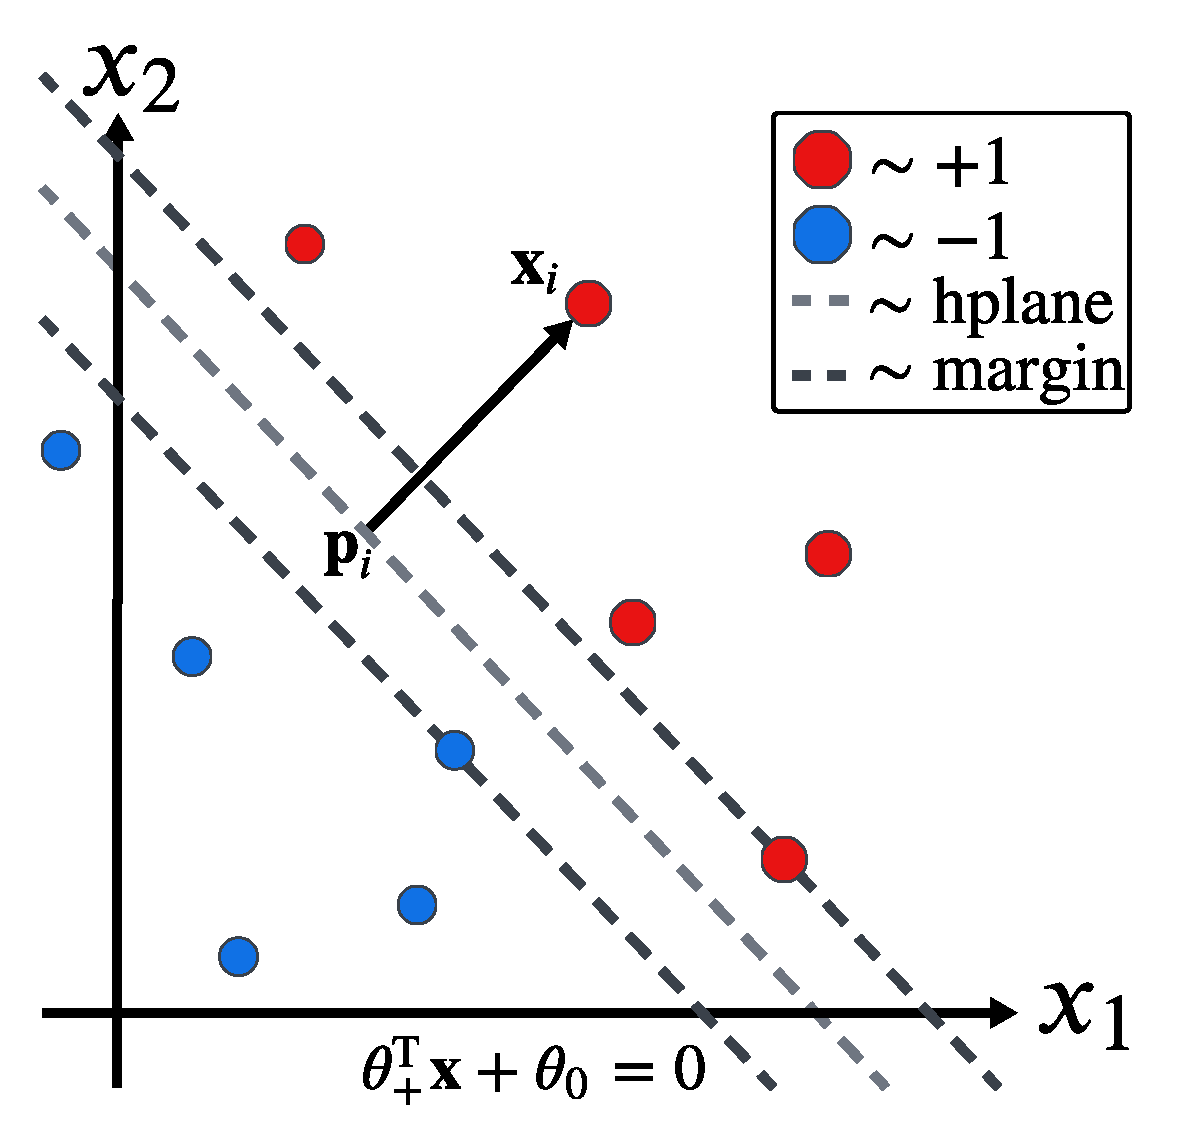
\includegraphics[width=\linewidth]{./figures/supervised_learning/SVM_hard_margin.pdf}
    \end{minipage}%
    \hfill
    \begin{minipage}{0.46\linewidth}
        \caption{A hard-margin SVM in two dimensions. Samples lying on the margin are referred to as support vectors.}
        \label{fig:SVM_hard_margin}
    \end{minipage}
\end{figure}

Let $\mathbf{p}_i$ denote the projection of $\x_i$ onto the hyperplane and let $d_i$ denote the distance between $\mathbf{p}_i$ and $\x_i$. Noting that the normal to the hyperplane is $\theta_+$, we have $\mathbf{p}_i=\x_i-\frac{\theta_+}{||\theta_+||}d_i$ and so
$$
\theta_+^\top \l(\x_i-\frac{\theta_+}{||\theta_+||}d_i\r)+\theta_0
=
0
$$
which, after some rearranging, yields
$$
d_i
=
\frac{\theta_+^\top \x_i+\theta_0}{||\theta_+||}.
$$
Similarly, taking a point $\x_i$ whose class is $-1$ yields $d_i=-\frac{\theta_+^\top \x_i+\theta_0}{||\theta_+||}$ and so a neater way of writing this distance for an arbitrary sample $\x_i$ is $d_i=\frac{y_i(\theta_+^\top \x_i+\theta_0)}{||\theta_+||}$. Hard-margin SVMs are only applicable to linearly sparable data and their construction, from data, effectively boils down to finding which parameters maximise $\min_{i=1,\dots,n}d_i$. That is, we seek to compute
\begin{align*}
    \theta^{*}
    &=
    \argmax_{(\theta_0,\theta_+)}\l[\min_{i=1,\dots,n}d_i\r]\\
    &=
    \argmax_{(\theta_0,\theta_+)}\l[\min_{i=1,\dots,n}\frac{y_i(\theta_+^\top \x_i+\theta_0)}{||\theta_+||}\r]
\end{align*}
which we'd like to translate into a convex optimisation problem. First, notice that computing $\theta^{*}$ is equivalent to solving
$$
\max_{(\theta_0,\theta_+)}\frac{r}{||\theta_+||}\text{ s.t. } y_i\l(\theta_+^\top \x_i+\theta_0\r)\geq r\text{ } (i=1,\dots,n).
$$
in which $r$ may be scaled arbitrarily by positives, so it is equivalent to
$$
\max_{(\theta_0,\theta_+)}\frac{1}{||\theta_+||}\text{ s.t. } y_i\l(\theta_+^\top \x_i+\theta_0\r)\geq 1\text{ } (i=1,\dots,n).
$$
This problem is still non-convex so we make a convenient switcheroo in realising that it is equivalent to solving
$$
\min_{(\theta_0,\theta_+)}||\theta_+||^2\text{ s.t. } y_i\l(\theta_+^\top \x_i+\theta_0\r)\geq 1\text{ } (i=1,\dots,n)
$$
which is solved in the usual convex problem solving ways.

\subsubsection{Soft-margin SVMs}

Hard-margin SVMs are rarely applicable. In practice, samples are not entirely linearly separable and so allowing for some misclassification is pragmatic. Going from hard-margin to soft-margin is pretty straightforward, just include some slack variables $\xi=(\xi_1,\dots,\xi_n)$ that ultimately allow the model to violate the constraints while penalising said violations. More precisely, it involves solving
$$
\min_{(\theta_0,\theta_+,\xi)}\l[||\theta_+||^2+\lambda\sum_{i=1}^n\xi_i\r]\text{s.t. } y_i\l(\theta_+^\top \x_i+\theta_0\r)\geq 1-\xi_i,\text{ }\xi_i\geq0
$$
for $i=1,\dots,n$ where $\lambda\geq0$ is a regularisation parameter that influences the tradeoff of margin size and misclassification rate. Larger $\lambda$ corresponds to prioritising a larger margin while smaller $\lambda$ corresponds to prioritising the minimisation of misclassification.

\begin{figure}[t]
    \centering
    \begin{minipage}{0.54\linewidth}
        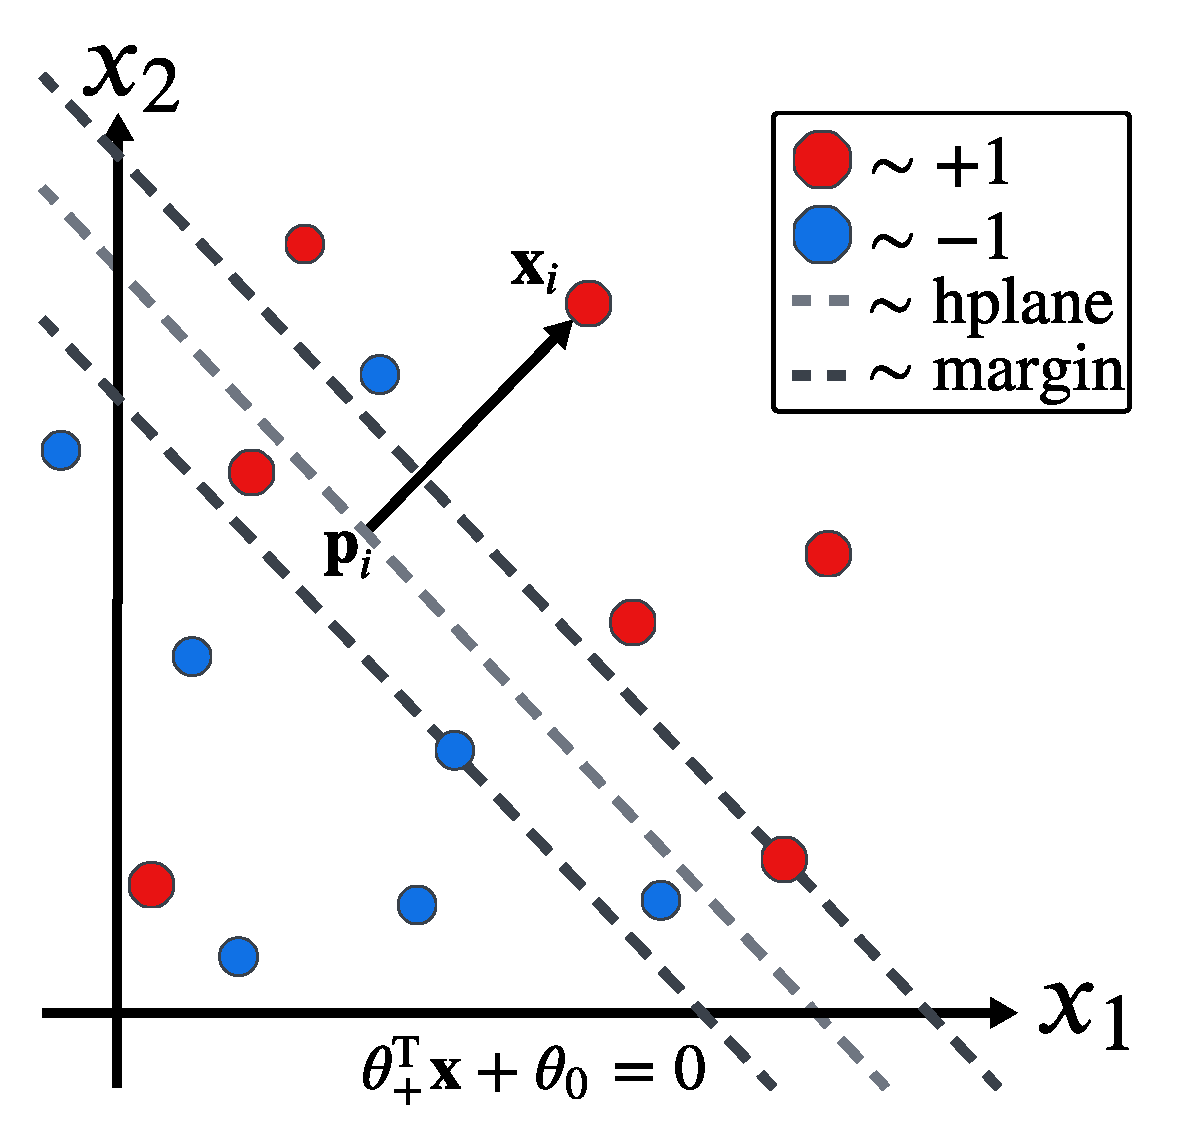
\includegraphics[width=\linewidth]{./figures/supervised_learning/SVM_soft_margin.pdf}
    \end{minipage}%
    \hfill
    \begin{minipage}{0.46\linewidth}
        \caption{A soft-margin SVM in two dimensions. Samples are labelled according to their true class.}
        \label{fig:SVM_soft_margin}
    \end{minipage}
\end{figure}

As illustrated in \autoref{fig:SVM_soft_margin}, it allows for samples to be closer to the decision boundary than the margin as well as outright misclassifications. Again, it is typically solved in the usual convex problem solving ways. Going a step further, it turns out that this can be reduced to computing
$$
\argmin_{(\theta_0,\theta_+)}\l[||\theta_+||^2+\lambda\sum_{i=1}^n\max\l(0,1-y_i\l(\theta_+^\top \x_i+\theta_0\r)\r)\r]
$$
which can be done using gradient descent.

\subsubsection{Non-linear SVMs}
Motivating non-linear SVMs is straightforward: we'd sometimes like to separate samples by a non-linear decision boundary. With this in mind, a super intuitive approach is to find a transformation $\phi$ which maps samples to a space in which they are linearly separable. In said space, employ a linear SVM.

% \begin{figure}[t]
%     \centering
%     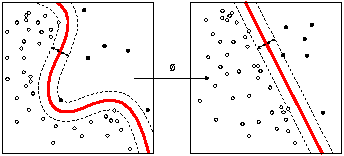
\includegraphics[width=0.75\columnwidth]{./figures/supervised_learning/SVM_non_linear.pdf}
%     \caption{Non-linearly separable data being transformed into linearly separable data.}
%     \label{fig:SVM_non_linear}
% \end{figure}

\begin{figure}[t]
    \centering
    \begin{minipage}{0.59\linewidth}
        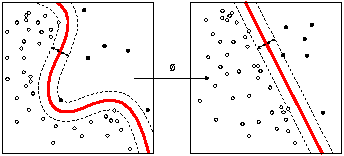
\includegraphics[width=\linewidth]{./figures/supervised_learning/SVM_non_linear.pdf}
    \end{minipage}%
    \hfill
    \begin{minipage}{0.4\linewidth}
        \caption{Non-linearly separable data being transformed into linearly separable data.}
        \label{fig:SVM_non_linear}
    \end{minipage}
\end{figure}

With this idea in mind, we seek to solve
$$
\min_{(\theta_0,\theta_+,\xi)}\l[\frac{1}{2}||\theta_+||^2+\lambda\sum_{i=1}^n\xi_i\r]\text{s.t. } y_i\l(\phi(\theta_+)^\top\x_i+\theta_0\r)\geq 1-\xi_i,\text{ }\xi_i\geq0
$$
which is difficult if the dimension of the image of $\phi$ is large. To make things easier, the dual of problem is optimised instead. My understanding of primal problems and their dual problems isn't great, so I'll just give the dual outright without deriving it:
$$
\max_{(\alpha_1,\dots,\alpha_n)\in[0,\lambda]^n}\l[\sum_{i=1}^n\alpha_i-\frac{1}{2}\sum_{i=1}^n\sum_{j=1}^n\alpha_i\alpha_jy_iy_jK(\x_i,\x_j)\r]\text{s.t. }\sum_{i=1}^n\alpha_iy_i=0
$$
where $K(\x,\z)=\langle\phi(\x),\phi(\z)\rangle$ is a pre-chosen kernel. See how it never requires an explicit computation involving $\phi$ as long as a closed form of $K(\x,\z)$ not involving $\phi$ is available. This is referred to as the kernel trick and reduces having to solve an optimisation problem in a space whose dimension is the number of features to a space whose dimension is the number of training samples.

At inference time, given some $\x$, we seek to compute
\begin{align*}
    y
    &=
    \text{sign}\l(\theta_+^\top\phi(\x)+\theta_0\r)\\
    &=
    \text{sign}\l(\sum_{i=1}^n\alpha_iy_iK(\x_i,\x)+b_k\r)
\end{align*}
where $b_k=y_k-\sum_{i=1}^n\alpha_iy_iK(\x_i,\x_k)$ for some $(\x_k,y_k)$ that satisfies $\alpha_k\in(0,\lambda)$. Note that the second line in the equation above is derived using to argument made in deriving the dual.

The two simplest kernels are polynomial kernels and the radial basis function (RBF) kernel, the latter of which is far more popular. That said, polynomial kernels have had their place in applying SVMs to natural language processing tasks. The polynomial kernels
$$
K(\x,\z)
=
(\x^\top\z+c)^d
$$
capture feature interactions up to degree $d$, which is useful when the separation of classes depends on combinations of input variables, e.g. quadratic boundaries in $\mathbb{R}^2$. Therein lies their weakness: polynomial kernels can be limited if said decision boundary is particuarly irregular. The RBF kernel
$$
K(\x,\z)
=
\exp\l(-\frac{||\x-\z||^2}{2\sigma^2}\r)
$$
is more flexible as a result of it measuring similarity based on distance, effectively producing localised bumps in feature space. From this, the model is able to form very non-linear decision boundaries. So, all in all, polynomial kernels provide interpretable higher-order interactions, while RBF kernels offer universal approximation.

% decision trees and random forests
\subsection{Decision Trees and Random Forests}
I find decision trees and random forests so boring that I'm not going to write about them and will instead point to \autoref{fig:random_forest} which illustrates random forests well. This section mostly exists so that the list of subsections in this section form a well-rounded list of supervised learning methods.

\begin{figure}[t]
    \centering
    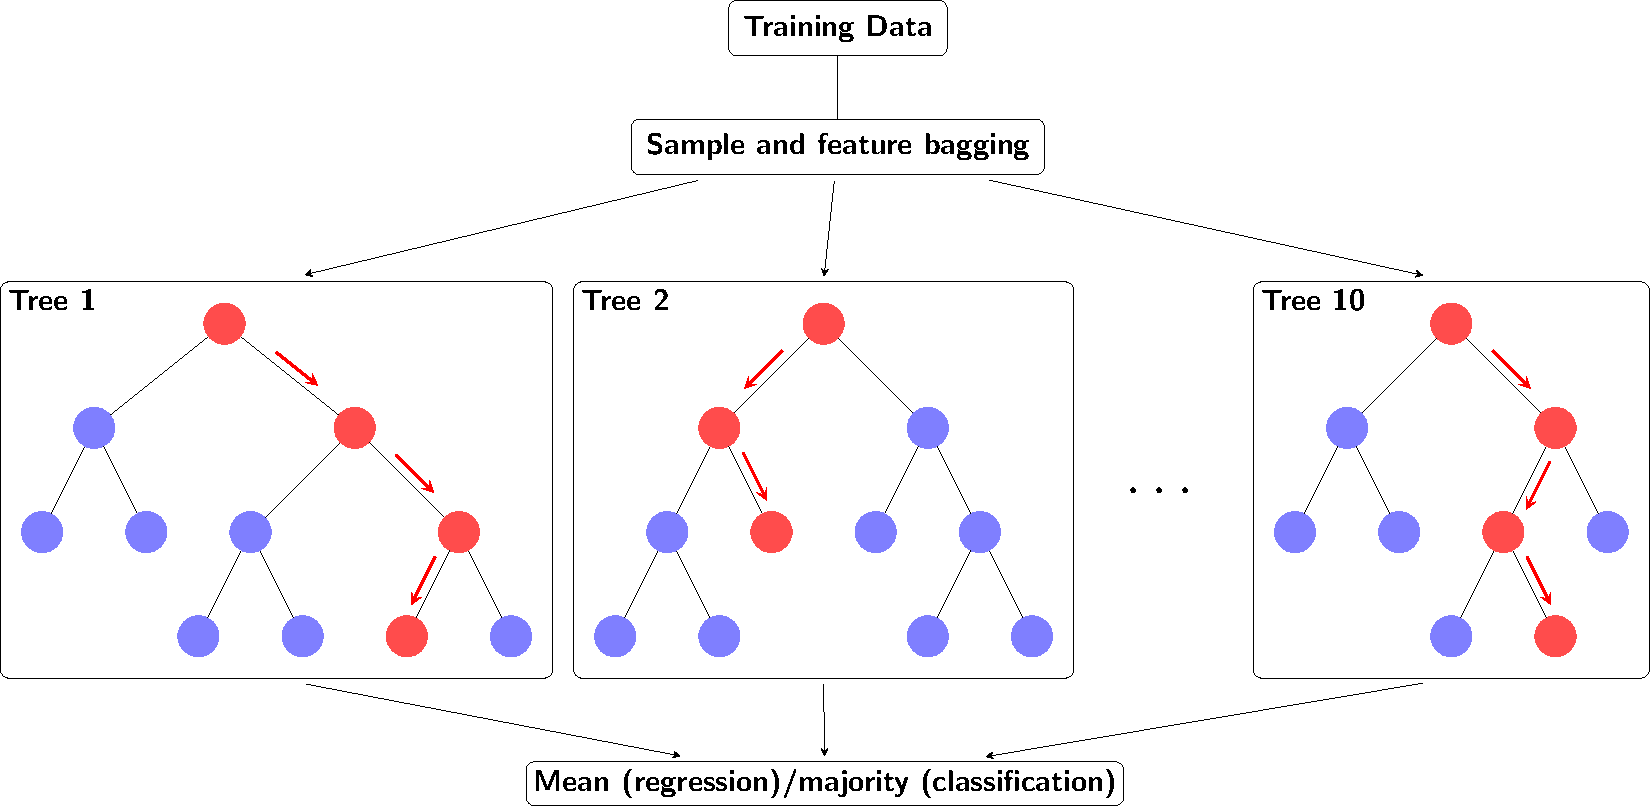
\includegraphics[width=\columnwidth]{./figures/supervised_learning/random_forest.pdf}
    \caption{A random forest.}
    \label{fig:random_forest}
\end{figure}

Despite my disinterest in them, learning about decision trees encourages you to understand entropy which is good. There are other topics which encourage the same thing though, e.g. Variational Autoencoders, through the use of KL-divergences. Also, random forests are a nice introduction to ensemble methods which nicely demonstrate how to prevent overfitting by reducing variance — directly illustrating the importance of the bias-variance tradeoff! Oh, and bootstrapping. One day I'll write this subsection properly.

\begin{tcolorbox}[title={\centering\textbf{Logistic regression $>$ SVM/RF when?}}, colback=myLightBlue, colbacktitle=myDarkBlue, colframe=myDarkBlue, coltitle=white]
    This is a pretty natural question once shown more sophisticated methods which deal with linearly separable and non-linearly separable data. The largest benefit of logistic regression is that it allows for statistical significance tests on parameters. It also helps that its implementation and interpretation are straightforward.
\end{tcolorbox}

% the bias-variance tradeoff
\subsection{The Bias-Variance Tradeoff}
The bias-variance tradeoff is a statement pertaining to the goodness of estimators (learning algorithms) according to mean square error (MSE) in terms of their variance — with respect to training data — and the square of their bias — due to architecture-related assumptions. It turns out that the optimal estimator, according to mean square error, is a careful tradeoff of both. Before deriving the tradeoff, let's consider the consequences of high squared bias and high variance: underfitting and overfitting.

\subsubsection{Underfitting and Overfitting}
Crudely put, if the architecture pertaining to an estimator is too simple to represent the point estimate then the estimator's bias (and thus its square) will be large in magnitude. Such an estimator underfits that which it is intended to model. I like to think of such an estimator as being almost invariant to the training data. As a practical example, think of fitting a line to a very non-linear function as in the leftmost plots of \autoref{fig:fitting_under} and \autoref{fig:fitting_over}. Underfitting is reflected during training by both high training error and high validation error.

At the other extreme, if the architecture pertaining to an estimator is more complex than is necessary (e.g. overparameterised) to represent the point estimate then the excess parameters often\footnote{See the double-descent phenomenon in \autoref{fig:double_descent}.} cause the model to fit the noise in the training data. In this case, the estimator is highly variant with respect to the training data. Such an estimator overfits the training data instead of fitting the point estimate. As a practical example, think of fitting a polynomial from small and heavily-noised training data, as in the rightmost plot of \autoref{fig:fitting_over}. Overfitting is reflected during training by low training error and high validation error (relative to the training error).

\begin{figure}[t]
    \centering
    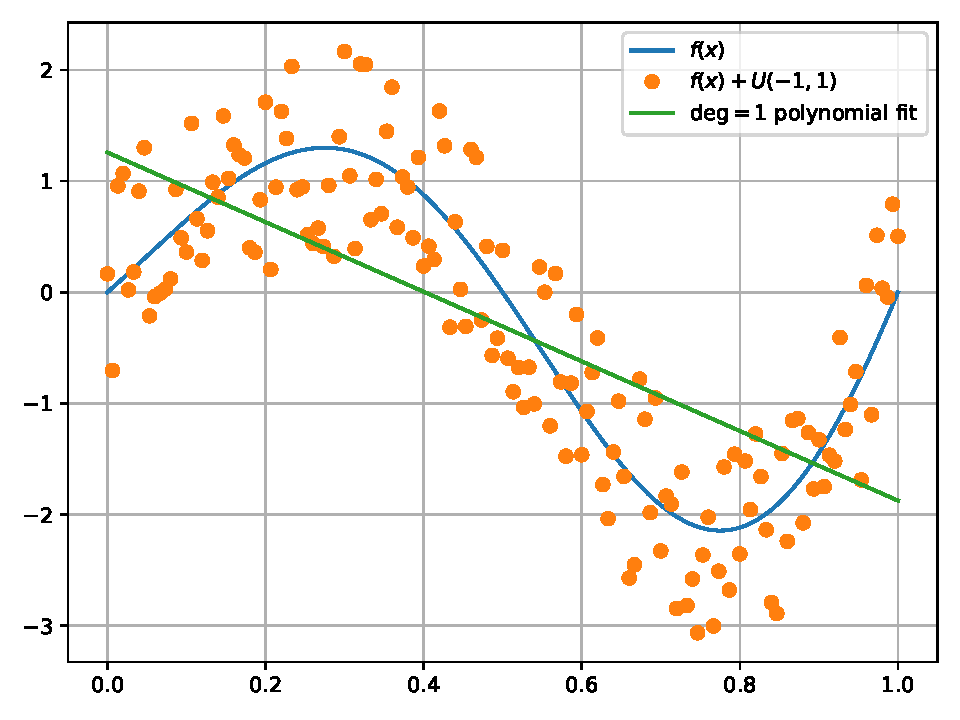
\includegraphics[width=0.32\columnwidth]{./figures/supervised_learning/fitting_under_M=1.pdf}
    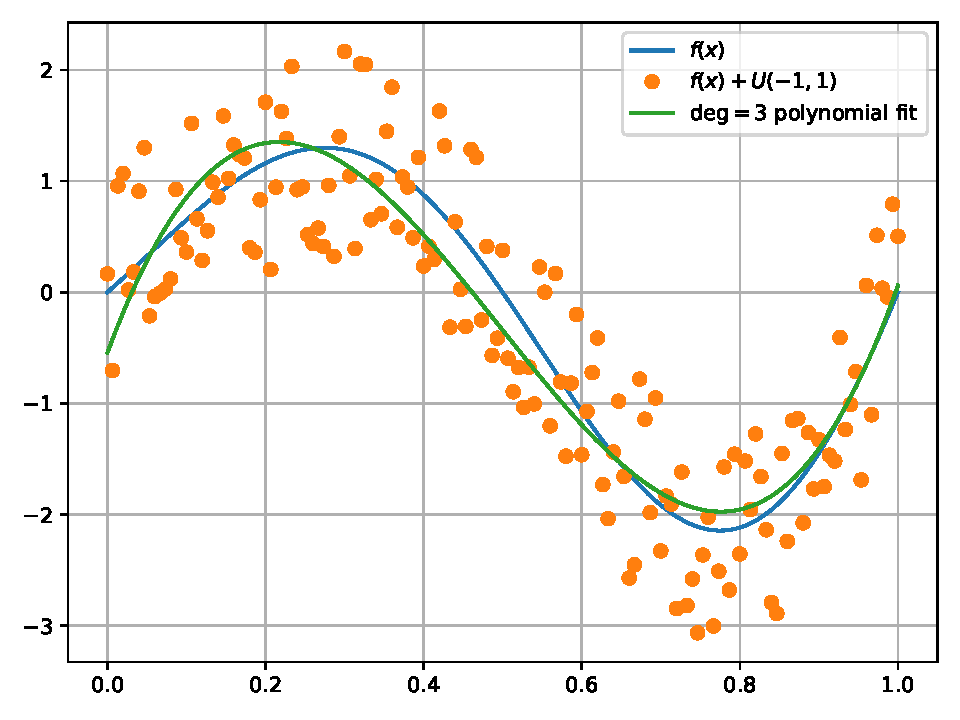
\includegraphics[width=0.32\columnwidth]{./figures/supervised_learning/fitting_under_M=3.pdf}
    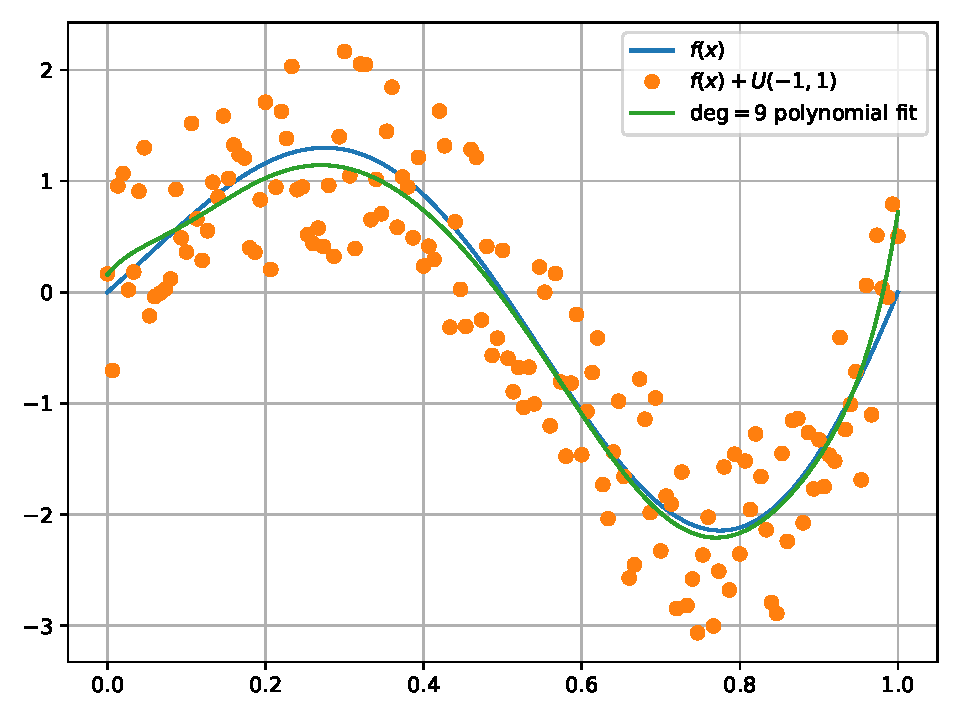
\includegraphics[width=0.32\columnwidth]{./figures/supervised_learning/fitting_under_M=9.pdf}
    \caption{Lots of data, little noise.}
    \label{fig:fitting_under}
\end{figure}

\begin{figure}[t]
    \centering
    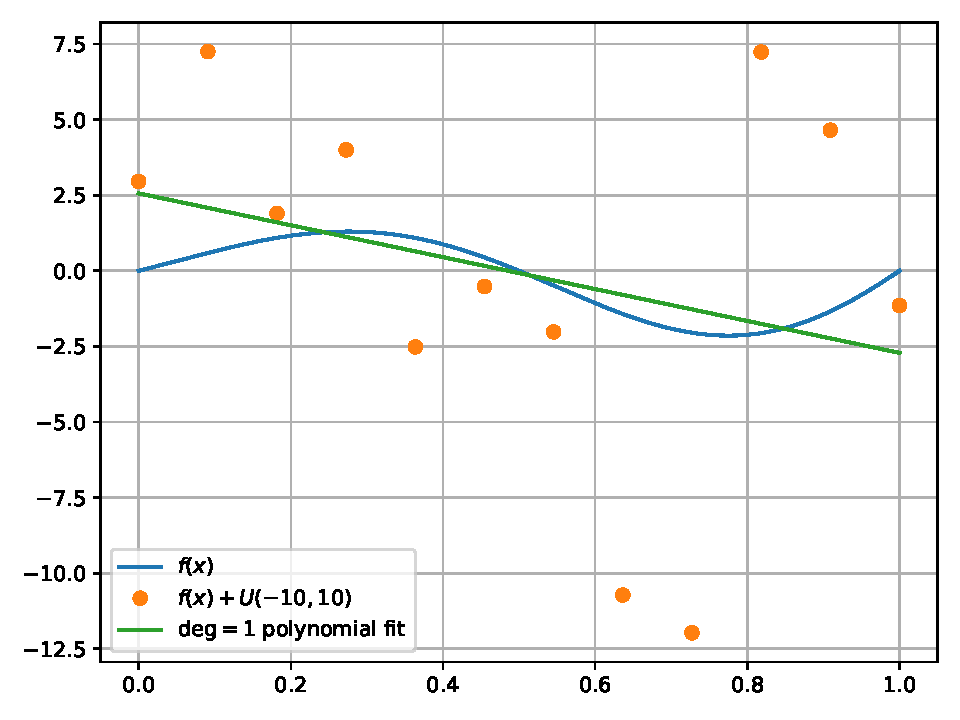
\includegraphics[width=0.32\columnwidth]{./figures/supervised_learning/fitting_over_M=1.pdf}
    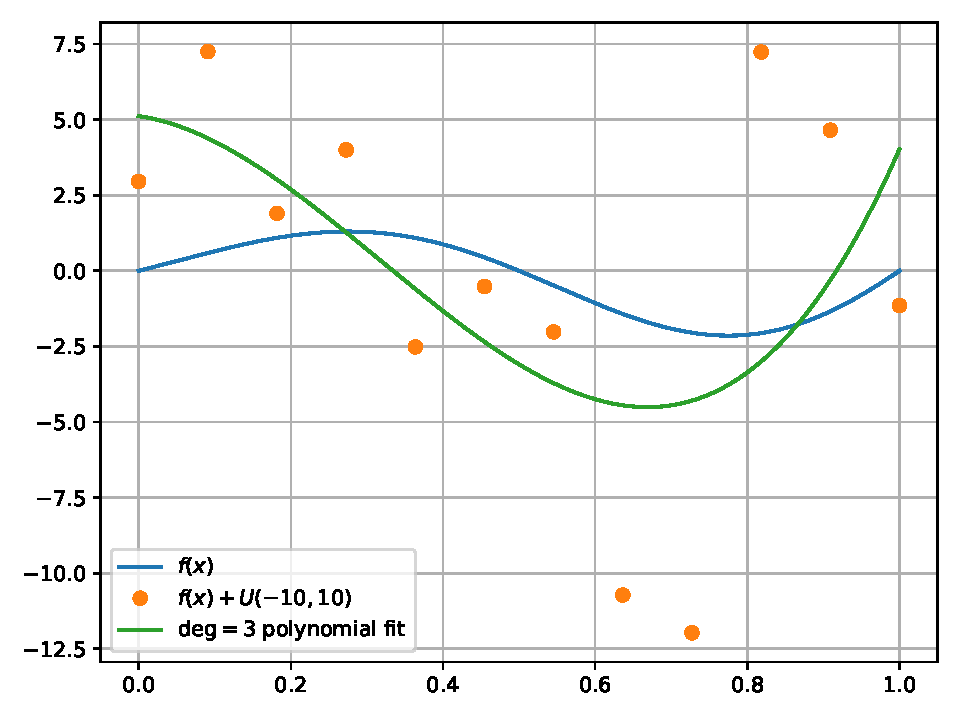
\includegraphics[width=0.32\columnwidth]{./figures/supervised_learning/fitting_over_M=3.pdf}
    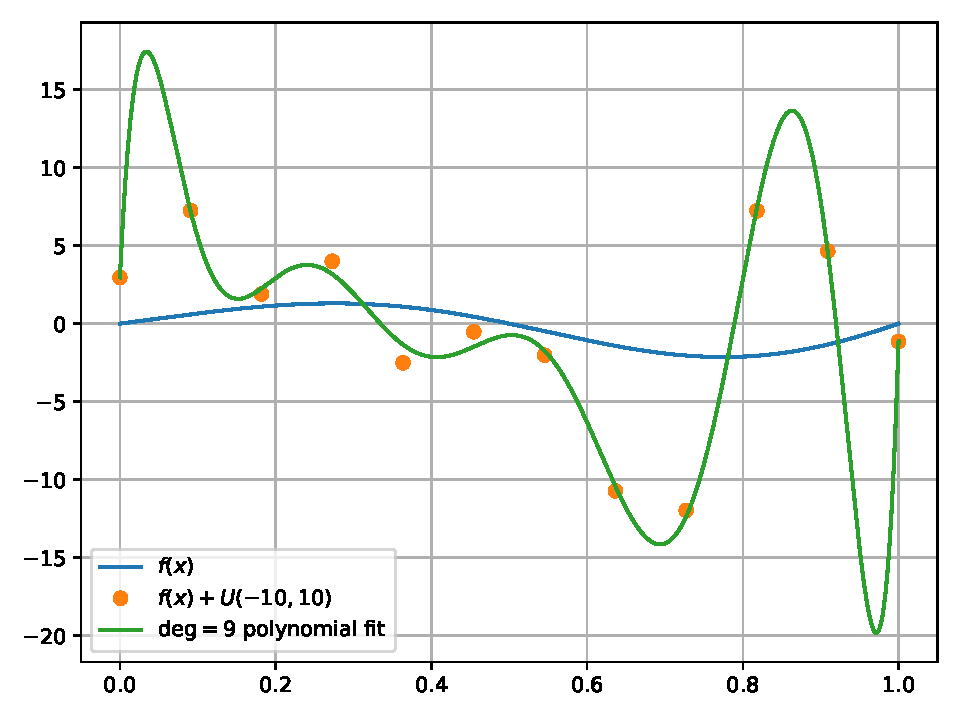
\includegraphics[width=0.32\columnwidth]{./figures/supervised_learning/fitting_over_M=9.pdf}
    \caption{Little data, lots of noise.}
    \label{fig:fitting_over}
\end{figure}

\subsubsection{Derivation with MSE loss}
Recall that target values are often effected by noise, i.e. $Y|(\X=\x)=f(\x)+\epsilon(\x)$ where $\epsilon(\x)\sim\mathcal{N}(0,\sigma^2(\x))$ and so
$$
Y|(\X=\x)
\sim
\mathcal{N}\l(f(\x), \sigma^2(\x)\r).
$$
Given a fixed architecture, the estimate $\hat{f}_D$ of $f$ is a purely function of the training dataset $D\subset(\Omega_{\X}\times\Omega_Y)^n$. Such a dataset is a realisation of the random variable $\D$ distributed according to $p(\x,y)^{\otimes n}$. In line with this, the bias and variance derived are that of the estimator $f_{\D}$.

As is common in regression contexts, the goodness of an estimate $\hat{f}_D$ is given by its expected risk
$$
R\l(\hat{f}_D\r)
=
\E_{(\X,Y)}\l[\l(Y-\hat{f}_D(\X)\r)^2\r]
$$
in which mean square error (MSE) is used as loss. Thus, the quality of the corresponding estimator (or learning algorithm) used to determine $\hat{f}_{D}$ from $D\in\Omega_{\D}$ is given by
\begin{align*}
    &\hspace{14.52pt}
    \E_{\D}\l[R\l(\hat{f}_{\D}\r)\r]\\
    &=
    \E_{\D}\l[\E_{(\X,Y)}\l[\l(Y-\hat{f}_{\D}(\X)\r)^2\r]\r]\nonumber\\
    &=
    \E_{\D}\l[\E_{(\X,Y)}\l[\l(Y-f(\X)+f(\X)-\hat{f}_{\D}(\X)\r)^2\r]\r]\nonumber\\
    &=
    \textcolor{myYellow}{\E_{\D}\l[\E_{(\X,Y)}\l[\l(Y-f(X)\r)^2\r]\r]}+
    \textcolor{myGreen}{\E_{\D}\l[\E_\X\l[\l(f(\X)-\hat{f}_{\D}(\X)\r)^2\r]\r]}\\
    &+\textcolor{myLightRed}{\E_{\D}\l[\E_{(\X,Y)}\l[2(Y-f(\X))\l(f(\X)-\hat{f}_{\D}(\X)\r)\r]\r]}.
\end{align*}
Let's address this term-by-term beginning with the term in red. See that
\begin{align*}
    &\hspace{14.52pt}
    \textcolor{myLightRed}{\E_{\D}\l[\E_{(\X,Y)}\l[2(Y-f(\X))\l(f(\X)-\hat{f}_{\D}(\X)\r)\r]\r]}\\
    &=
    2\E_{\D}\l[\E_\X\l[\E_{Y|\X}\l[(Y-f(\X))\l(f(\X)-\hat{f}_{\D}(\X)\r)\r]\r]\r]\\
    &=
    2\E_{\D}\l[\E_\X\l[\l(f(\X)-\hat{f}_{\D}(\X)\r)\E_{Y|\X}\l[Y-f(\X)\r]\r]\r]\\
    &=
    2\E_{\D}\l[\E_\X\l[\l(f(\X)-\hat{f}_{\D}(\X)\r)\cdot0\r]\r]\\
    &=
    0
\end{align*}
in which the tower property of conditional expectations
\begin{align*}
    \E_{(\X,Y)}[g(\X,Y)]
    &=
    \iint g(\x,y)f_{(\X,Y)}(\x,y)dxdy\\
    &=
    \int \l(\int g(\x,y)f_{Y|\X}(y|\x)dy\r)f_\X(\x)dx\\
    &=
    \E_\X\l[\E_{Y|\X}\l[g(\X,Y)\r]\r]
\end{align*}
is applied. As such, the quantity of interest reduces to only two terms as in
$$
\E_{\D}\l[R\l(\hat{f}_{\D}\r)\r]
=
\textcolor{myYellow}{\E_{\D}\l[\E_{(\X,Y)}\l[\l(Y-f(\X)\r)^2\r]\r]}+\textcolor{myGreen}{\E_{\D}\l[\E_\X\l[\l(f(\X)-\hat{f}_{\D}(\X)\r)^2\r]\r]}
$$
of which we will now address the first in orange. Noting that
$$
\E_{Y|(\X=\x)}\l[Y-f(\x)\r]
=
0
$$
for all $\x\in\Omega_{\X}$ and that what is inside the expectation over $\D$ is independent of $\D$, we see that the first term reduces to
\begin{align*}
    \textcolor{myYellow}{\E_{\D}\l[\E_{(\X,Y)}\l[(Y-f(\X))^2\r]\r]}
    &=
    \E_{(\X,Y)}\l[(Y-f(\X))^2\r]\\
    &=
    \E_\X\l[\E_{Y|\X}\l[(Y-f(\X))^2\r]\r]\\
    &=
    \E_\X\l[\E_{Y|\X}\l[\l(Y-\E_{Y|\X}[Y]\r)^2\r]\r]\\
    &=
    \E_\X\l[\text{Var}\l(Y|\X\r)\r]\\
    &=
    \E_\X[\sigma^2(\X)]
\end{align*}
This is simply the expected noise, e.g. due to imperfect calibration in the instruments used to obtain samples.

To address the term in green, let $\bar{f}(\x)=\E_{\D}\l[\hat{f}_{\D}(\x)\r]$ for all $\x\in\Omega_\X$ and see that
\begin{align*}
    &\hspace{14.52pt}
    \textcolor{myGreen}{\E_{\D}\l[\E_\X\l[\l(f(\X)-\hat{f}_{\D}(\X)\r)^2\r]\r]}\\
    &=
    \E_{\D}\l[\E_\X\l[\l(f(\X)-\bar{f}(\X)+\bar{f}(\X)-\hat{f}_{\D}(\X)\r)^2\r]\r]\\
    &=
    \E_\X\l[\l(f(\X)-\bar{f}(\X)\r)^2\r]+\E_{\D}\l[\E_\X\l[\l(\bar{f}(\X)-\hat{f}_{\D}(\X)\r)^2\r]\r]\\
    &+
    2\E_{\D}\l[\E_\X\l[\l(f(\X)-\bar{f}(\X)\r)\l(\bar{f}(\X)-\hat{f}_{\D}(\X)\r)\r]\r].
\end{align*}
See that the final term vanishes as $\E_{\D}\l[\bar{f}(\x)-\hat{f}_{\D}(\x)\r]=0$ for all $\x\in\Omega_{\X}$ and so
\begin{align*}
    &\hspace{14.52pt}
    \textcolor{myGreen}{\E_{\D}\l[\E_\X\l[\l(f(X)-\hat{f}_{\D}(\X)\r)^2\r]\r]}\\
    &=
    \E_\X\l[\l(f(\X)-\bar{f}(\X)\r)^2\r]+\E_{\D}\l[\E_\X\l[\l(\bar{f}(\X)-\hat{f}_{\D}(\X)\r)^2\r]\r]\\
    &=
    \E_\X\l[\l(f(\X)-\bar{f}(\X)\r)^2+\E_{\D}\l[\l(\bar{f}(\X)-\hat{f}_{\D}(\X)\r)^2\r]\r]\\
    &=
    \E_\X\l[\l(f(\X)-\E_{\D}\l[\hat{f}_{\D}(X)\r]\r)^2+\E_{\D}\l[\l(\hat{f}_{\D}(\X)-\E_{\D}\l[\hat{f}_{\D}(\X)\r]\r)^2\r]\r].
\end{align*}
Put together, we obtain
\begin{align*}
    &\hspace{14.52pt}
    \E_{\D}\l[R\l(\hat{f}_{\D}\r)\r]\\
    &=
    \E_\X\l[\l(f(\X)-\E_{\D}\l[\hat{f}_{\D}(\X)\r]\r)^2+\E_{\D}\l[\l(\hat{f}_{\D}(\X)-\E_{\D}\l[\hat{f}_{\D}(\X)\r]\r)^2\r]\r]+\sigma^2\\
    &=
    \E_\X\l[\text{Bias}\l(\hat{f}_{\mathcal{D}}(\X)\r)^2+\text{Var}\l(\hat{f}_{\mathcal{D}}(\X)\r)\r]+\sigma^2
\end{align*}
where $\sigma^2=\E_\X\l[\sigma^2(\X)\r]$ (ignore the poor choice of notation). With this in mind, it's clear that we do not seek the estimator $\hat{f}_{\D}$ which minimises expected square bias or expected variance individually. Instead, we seek the estimator which hits the sweet spot in minimising their sum. An illustration of this statement, as the estimator's architecture is made more complex, is given in \autoref{fig:bias_variance}.

\begin{figure}[t]
    \centering
    \begin{minipage}{0.64\linewidth}
        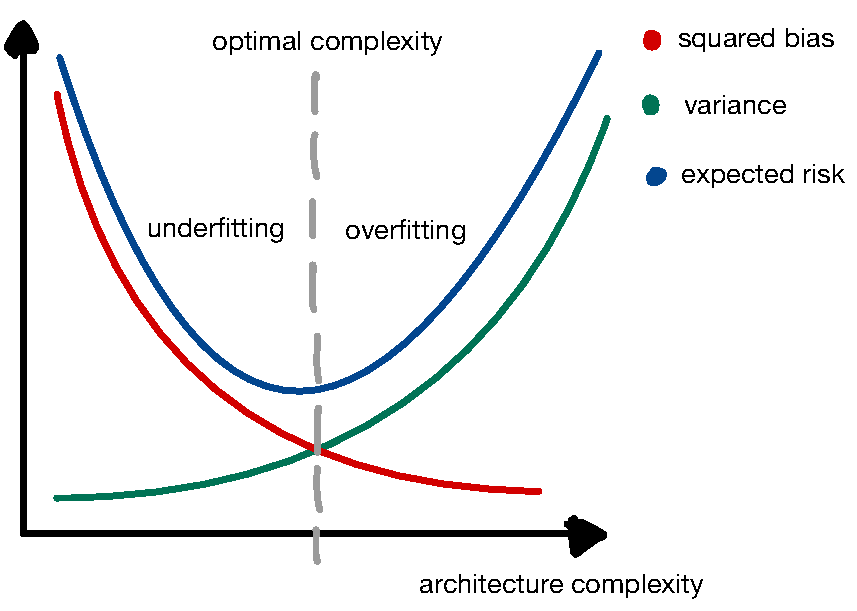
\includegraphics[width=\linewidth]{./figures/supervised_learning/bias_variance.pdf}
    \end{minipage}%
    \hfill
    \begin{minipage}{0.35\linewidth}
        \caption{Expected risk, squared bias and variance against architecture complexity.}
        \label{fig:bias_variance}
    \end{minipage}
\end{figure}

\begin{tcolorbox}[title={\centering\textbf{Beyond MSE}}, colback=myLightBlue, colbacktitle=myDarkBlue, colframe=myDarkBlue, coltitle=white]
    \textbf{Natural question:} MSE is a common choice of loss when dealing with regression but not classification, in which cross-entropies are typically used as loss, so why do derivations of the bias-variance tradeoff use MSE?
    
    \hspace{14.2pt} The quick answer is that it's the only choice which yields a relatively simple derivation of this elegant decomposition of estimator error into the square of its bias and its variance. I read online somewhere that some other choices of loss also yield decompositions into squared bias and variance but that their derivation is less elegant. There seems to be a good amount of work in this area but it's too in-depth for this document.
\end{tcolorbox}

\subsubsection{Double descent}
Double descent refers to a behaviour observed in select set ups in which overparameterised models seemingly fly in the face of the bias-variance tradeoff. As the number of parameters (i.e. the model complexity) increases, the test error increases in line with the usual bias-variance tradeoff until reaching the number of training samples $n$. At this point, the test error spikes and training error hits 0. That is, the model is able to entirely interpolate the training data. The phenomenon begins as the number of parameters exceeds $n$. Not only does training error remain 0 (expected) but the test error begins to decrease and, in many set ups, reduces to an amount below the minimum test error observed during the traditional bias-variance region.

The phenomenon is illustrated nicely in \autoref{fig:double_descent} and motivates the massively overparameterised contemporary models used these days. AlexNet is an example of an overparameterised model lying in the second descent region with around 60 million parameters but only 1.2 million training samples.

\begin{figure}[t]
    \centering
    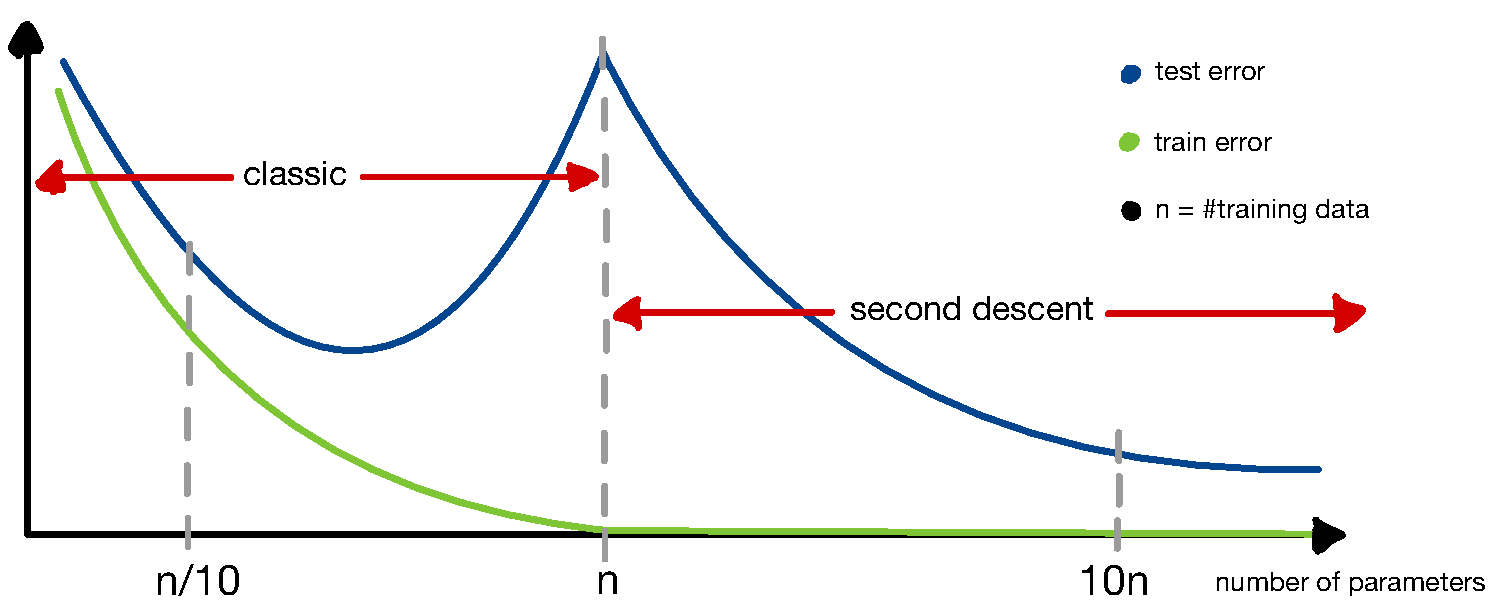
\includegraphics[width=1\columnwidth]{./figures/supervised_learning/double_descent.pdf}
    \caption{The double descent phenomenon, $n=|D_{\text{train}}|$.}
    \label{fig:double_descent}
\end{figure}

I like to imagine fitting a third degree polynomial by polynomials of higher and higher degree. If double descent were observed in this set up, one might expect wild polynomial fits until the polynomial's degree matches the number of training samples. At which point, the model has interoplated the training data perfectly and begins to regulate how it fits what's inbetween.

There has been a good amount of work investigating the phenomenon and some of the mystery has reduced as a result. The most convincing hand-wavy explanation of the behaviour is that parameter exploration via gradient descent is inherently regulatory. Not only that but the use of explcit regularisation, like SGD and Adam, on top of the self-regularisation bias toward parameters which offer `simpler' representations.

% parameter exploration and its optimisation
\section{Parameter Exploration and its Optimisation}
In fitting a parametric model $f_{\theta}:\Omega_{\X}\to\Omega_{Y}$, the loss induced by a choice of model parameters $\theta$ for a sample $(\x,y)$ is given by $\mathcal{L}\l(y,f_{\theta}(\x)\r)$ for some loss function $\mathcal{L}:\Omega_Y\times\Omega_Y\to\mathbb{R}_{\geq0}$. In line with this, let the empirical risk $R_D$ over a given dataset $D=\{(\x_i,y_i)\}_{i=1}^n$ be given by
\begin{align*}
    R_D:\Theta&\to\R_{\geq0}\\
    \theta&\mapsto\frac{1}{n}\sum_{i=1}^n\mathcal{L}(y_i,f_{\theta}(\x_i))
\end{align*}
In fitting $f_{\theta}$, we seek to compute
$$
\theta^{*}
=
\argmin_{\theta\in\Theta}R_D(\theta),
$$
i.e. to minimise the empirical risk over the dataset in the parameters. As such, methods of function minimisation are of interest.

\begin{figure}[t]
    \centering
    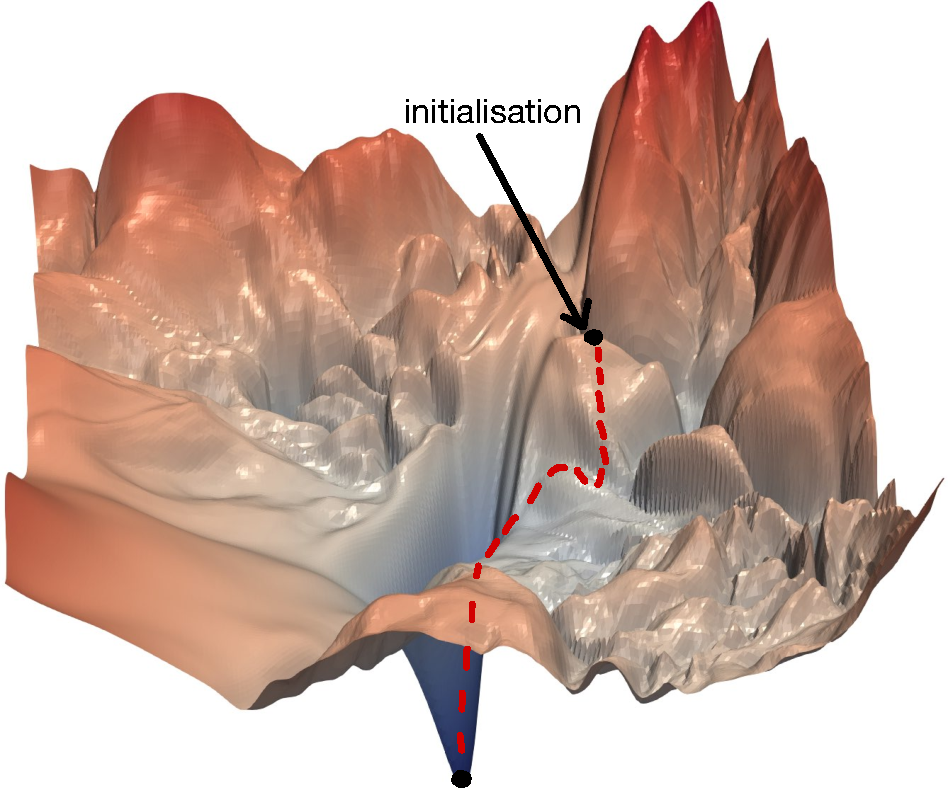
\includegraphics[width=0.7\linewidth]{./figures/gradient_descent/loss_landscape.pdf}
    \caption{The graph $\{(\theta,R_D(\theta))|\theta\in\R^2\}$ of a complex loss landscape and a visualisation of how me might hope gradient descent looks.}
    \label{fig:loss_landscape_complex}
\end{figure}

Many function minimisation methods exist: Newton's method, genetic algorithms, gradient descent, etc. but most are horribly slow/unstable in high dimensions; not gradient descent though! As a result, gradient descent is \textit{the} method for computing good parameters numerically in deep learning, hence the inclusion of this section.

\begin{tcolorbox}[title={\centering\textbf{Illustrations of loss landscapes are dataset-dependent!}}, colback=myLightBlue, colbacktitle=myDarkBlue, colframe=myDarkBlue, coltitle=white]
    When loss landscapes are illustrated, they are really plots of the graph $\{(\theta, R_D(\theta))|\theta\in\Theta\}$. That is, they are shaped by the fixed dataset $D$. As such, computations of the form $R_{D'}(\theta)$ for $D'\subsetneq D$, e.g. computations related to mini-batch or stochastic gradient descent, don't necessarily coincide with $R_D(\theta)$.
\end{tcolorbox}

% vanilla gradient descent
\subsection{Gradient Descent}
Since gradient descent is a general function minimisation method and not specific to machine learning, I'll use more general mathsy notation than $\theta$, $R_D$, etc.

Say we're interested in finding minima of a function $f$ whose co-domain is $\mathbb{R}_{\geq0}$. A natural idea is to start with a guess $\x^{(0)}$ and send it in the direction in which $f$ most decsends locally from $\x^{(0)}$, or equivalently the opposite of the direction in which $f$ most ascends locally from $\x^{(0)}$, i.e. computing
$$
\argmax_{||\mathbf{v}^{(0)}||=1}f\l(\x^{(0)}+\eta\mathbf{v}^{(0)}\r),
$$
for some small $\eta>0$, and updating our guess to $\x^{(1)}=\x^{(0)}-\eta\mathbf{v}^{(0)}$. Iteratively applying this idea yields the usual gradient descent rule
$$
\x^{(t+1)}
=
\x^{(t)}-\eta\mathbf{v}^{(t)}.
$$
Eventually, after taking a ton of these small steps, we hope to reach a minimum of $f$.

\subsubsection{In which direction does $f$ most ascend locally from $\x^{(t)}$?}
In the following physicist-like argument, we consider only unit vectors $\mathbf{v}$. This is because we care only about the direction of the vector in question and an equation later on simplifies quite nicely due to its unit length. 

\begin{tcolorbox}[title={\centering\textbf{Multivariate Taylor expansion}}, colback=myLightBlue, colbacktitle=myDarkBlue, colframe=myDarkBlue, coltitle=white]
    Recall that if $f:\R^m\to\R$ then its second order Taylor expansion about $\mathbf{a}\in\R^m$ is given by
    $$
    f(\x)
    =
    f(\mathbf{a})+\nabla f(\mathbf{a})\cdot(\x-\mathbf{a})+\frac{1}{2}(\x-\mathbf{a})\cdot\nabla^2 f(\mathbf{a})(\x-\mathbf{a}).
    $$
\end{tcolorbox}

In gradient ascent, we are looking for the unit vector $\mathbf{v}$ whose direction $f$ increases most locally from $\mathbf{x}$, i.e. we seek
$$\argmax_{||\mathbf{v}||=1}\Big[f(\mathbf{x}+\eta\mathbf{v})-f(\mathbf{x})\Big]$$
where $\eta>0$ is small. Approximating $f(\mathbf{x}+\eta\mathbf{v})$ using its Taylor expansion about $\x$ yields
$$
f(\mathbf{x}+\eta\mathbf{v})-f(\mathbf{x})
\approx
\nabla f(\mathbf{x})\cdot\eta\mathbf{v}.
$$
Thus, the problem translates to finding the unit vector $\mathbf{v}$ that maximises
$$
\nabla f(\mathbf{x})\cdot\eta\mathbf{v}=||\nabla f(\mathbf{x})||\cdot||\eta\mathbf{v}||\cdot\cos(\theta)=\eta||\nabla f(\mathbf{x})||\cdot\cos(\theta)
$$
where $\theta\in[0,\pi)$ denotes the angle between $\nabla f(\mathbf{x})$ and $\mathbf{v}$. This expression is maximised when $\cos(\theta)=1$, i.e. when $\theta=0$, which necessitates $\mathbf{v}$ having the same direction as $\nabla f(\mathbf{x})$. So $\mathbf{v}$ is a unit vector in the direction of $\nabla f(\mathbf{x})$, i.e. $\mathbf{v}=\frac{\nabla f(\mathbf{x})}{||\nabla f(\mathbf{x})||}$. To see that $f$ ascends after being sent in the direction of $\mathbf{v}=\frac{\nabla f(\mathbf{x})}{||\nabla f(\mathbf{x})||}$ from $\mathbf{x}$, note that
$$
f(\mathbf{x}+\eta\mathbf{v})-f(\mathbf{x})
\approx
\nabla f(\mathbf{x})\cdot\eta\mathbf{v}
=
\eta\frac{\nabla f(\mathbf{x})\cdot\nabla f(\mathbf{x})}{||\nabla f(\mathbf{x})||}
=
\eta||\nabla f(\mathbf{x})||
>
0.
$$
The edge case in which $\nabla f(\mathbf{x})=0$ corresponds to $f(\mathbf{x})$ being a local maximum.

\subsubsection{Sensitivity to $\x^{(0)}$}
I don't know much about initialisation. I know that it's a bad idea to start at 0 (if certain symmetries hold then parameters may change identically), points of large magnitude (exploding gradients) and points of small magnitude (vanshing gradients). Simon Price speaks of some interesting quirks of parameter initialisation around 01:08:00 in a \href{https://www.youtube.com/watch?v=sJXn4Cl4oww&list=PLwFLAA-F1PgpU9lgxOdhjILkMXUagGnea&ab_channel=MachineLearningStreetTalk}{YouTube interview}.

One day when my interest in initialisation is sparked, I'll write this part properly.

\subsubsection{Batch learning}
If your training dataset is huge and you don't have enough VRAM to store gradient information then do not fear! It turns out that we can approximate full gradient updates reasonably well using many smaller updates over subsets of the dataset. How well mini-batch learning and stochastic gradient descent perform (and even just \textit{that} they perform) surprised me when I first learned about them.

\begin{figure}[t]
    \centering
    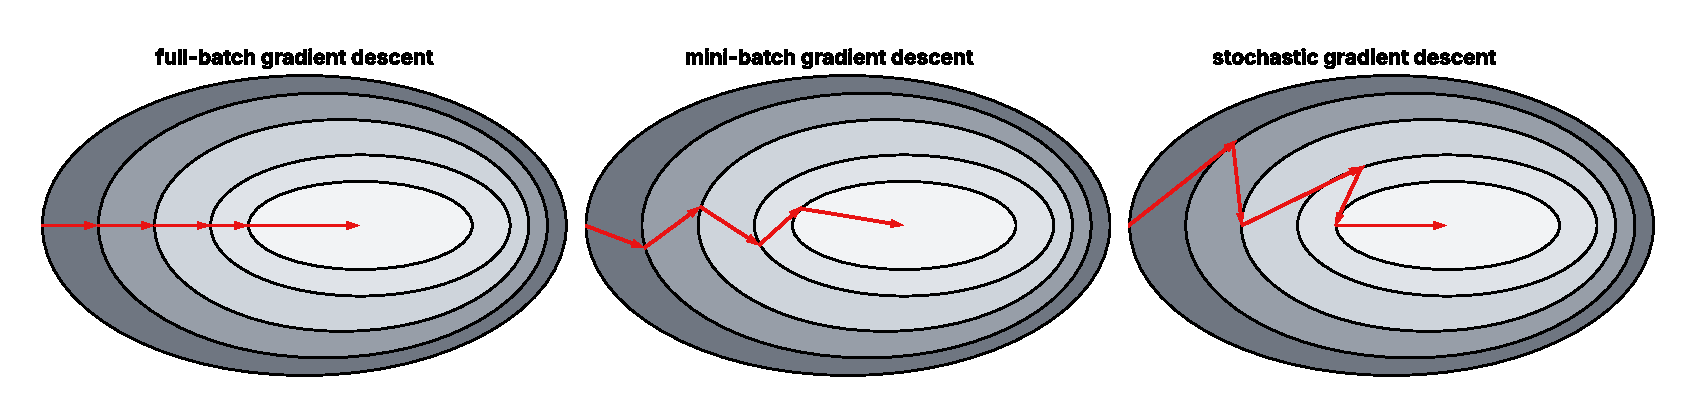
\includegraphics[width=\columnwidth]{./figures/gradient_descent/gradient_descent_types.pdf}
    \caption{How the convergence of each method might look.}
    \label{fig:gradient_descent_types}
\end{figure}

\begin{tcolorbox}[title={\centering\textbf{Epoch terminology}}, colback=myLightBlue, colbacktitle=myDarkBlue, colframe=myDarkBlue, coltitle=white]
    During training, the model tweaks its parameters based on training data. In practice, the model does so for the same sample many times. Each full cycle of the model having learned from the training data is called an epoch.
\end{tcolorbox}

\subsubsection*{1) Full-batch}
Full-batch gradient descent involves one parameter update per epoch as in
$$
\theta^{(t+1)}
=
\theta^{(t)}-\frac{1}{n}\sum_{i=1}^n \nabla_{\theta}\mathcal{L}\l(y_i,f_{\theta^{(t)}}(\x_i)\r).
$$

\subsubsection*{2) Mini-batch}
The information stored in order to compute gradients during training might be too much for your PC's VRAM. If so, instead perform mini-batch gradient descent in which the dataset $D$ is partitioned into $m$ disjoint subsets $B_1,\dots,B_m$, referred to as batches, and $m$ parameter updates are made according to
$$
\theta^{(t+j)}
=
\theta^{(t+j-1)}-\frac{1}{|B_j|}\sum_{(\x,y)\in B_j} \nabla_{\theta}\mathcal{L}\l(y,f_{\theta^{(t+j-1)}}(\x)\r).
$$
We see that if we split into $m$ batches then a full epoch during training corresponds to $m$ parameter updates (or optimisation steps).

\subsubsection*{3) Stochastic gradient descent (SGD)}
It turns out that updating based on a single sample $(\x,y)$ (uniformly randomly sampled), as in
$$
\theta^{(t+1)}
=
\theta^{(t)}-\nabla_{\theta}\mathcal{L}\l(y,f_{\theta^{(t)}}(\x)\r)
$$
is viable. This surprised me a ton when I first read about it: I would have thought that it'd produce nonsense parameters. Unsurprisingly, SGD yields relatively unstable convergence, a bit like the steps that a drunk man would take in walking down a hill.

\begin{tcolorbox}[title={\centering\textbf{Terminology warning}}, colback=myLightBlue, colbacktitle=myDarkBlue, colframe=myDarkBlue, coltitle=white]
    What we call mini-batch gradient here is referred to by some as stochastic gradient descent. Confusing.
\end{tcolorbox}

\subsubsection{Batch + Layer normalisation}
I've only seen these forms of normalisation apply to training neural networks. I'm unaware of them being grounded in theory. They're very widley used so I've included them.

\subsubsection*{1) Batch norm}
For a batch $B=\{\x_1,\dots,\x_m\}$, batch normalisation is the act of normalising the post-activation values of some layer of $d$ neurons in a neural network. Denote the $d$ activation values for the sample $\x_i\in B$ as $(a_{i,1},\dots,a_{i,d})$. The entire batch's activation values for said layer can be written as a matrix as in
$$
\begin{bmatrix}
    a_{1,1} & \dots  & a_{1,d}\\
    \vdots  & \ddots & \vdots \\
    a_{m,1} & \dots  & a_{m,d}
\end{bmatrix}.
$$
Batch norm first normalises the columns of $A$ as in
$$
\begin{bmatrix}
    \hat{a}_{1,1} & \dots  & \hat{a}_{1,d}\\
    \vdots        & \ddots & \vdots       \\
    \hat{a}_{m,1} & \dots  & \hat{a}_{m,d}
\end{bmatrix}
=
\begin{bmatrix}
    (a_{1,1}-\mu_1) / \sqrt{\sigma_1^2+\epsilon} & \dots & (a_{1,d}-\mu_d) / \sqrt{\sigma_d^2+\epsilon}\\
    \vdots & \ddots & \vdots \\
    (a_{m,1}-\mu_1) / \sqrt{\sigma_1^2+\epsilon} & \dots & (a_{m,d}-\mu_d) / \sqrt{\sigma_d^2+\epsilon}
\end{bmatrix}
$$
where $\mu_j=\frac{1}{m}\sum_{i=1}^ma_{i,j}$, $\sigma_j^2=\frac{1}{m}\sum_{i=1}^m(a_{i,j}-\mu_j)^2$ and $\epsilon>0$ is small, appearing for the sake of computational stability. At this point, the columns have mean 0 and variance 1. The output of batch norm for sample $i\in\{1,\dots,m\}$ is given by
$$
(\gamma_1\hat{a}_{i,1}+\beta_1,\dots,\gamma_d\hat{a}_{i,d}+\beta_d)
$$
where $\gamma_1,\dots,\gamma_d$ and $\beta_1,\dots,\beta_d$ are learnable parameters.

I don't think that the effect of batch norm is immediately clear and the informal explanations given in the paper which introduced it have been largely discarded since. Perhaps it helps avoid exploding/vanishing gradients, I honestly don't know lol.

\subsubsection*{2) Layer norm}
If batch statistics aren't particularly meaningful or batch size is small then layer norm may be preferable. Layer norm applies to individual samples, as opposed to entire batches, and so normalises over the features instead. Given activation values $a_1,\dots,a_d$, layer norm first normalises the activation values as in
$$
(\hat{a}_1,\dots,\hat{a}_d)
=
\l(\frac{a_1-\mu}{\sqrt{\sigma^2+\epsilon}},\dots,\frac{a_d-\mu}{\sqrt{\sigma^2+\epsilon}}\r)
$$
where $\mu=\frac{1}{d}\sum_{j=1}^da_j$ and $\sigma^2=\frac{1}{d}\sum_{j=1}^d(a_j-\mu)^2$. Then, as in batch norm, we scale and shift to obtain
$$
(\gamma_1\hat{a}_1+\beta_1,\dots,\gamma_d\hat{a}_d+\beta_d)
$$
where $\gamma_1,\dots,\gamma_d$ and $\beta_1,\dots,\beta_d$ are learnable parameters. As with batch norm, I honestly don't know the influence layer norm has on training.

% regularisation
\subsection{Regularisation}
Overfitting is a pain. How might we regulate the learning procedure in a way that (hopefully) prevents overfitting? Regularisation!

\begin{figure}[t]
    \centering
    \begin{minipage}{0.44\linewidth}
        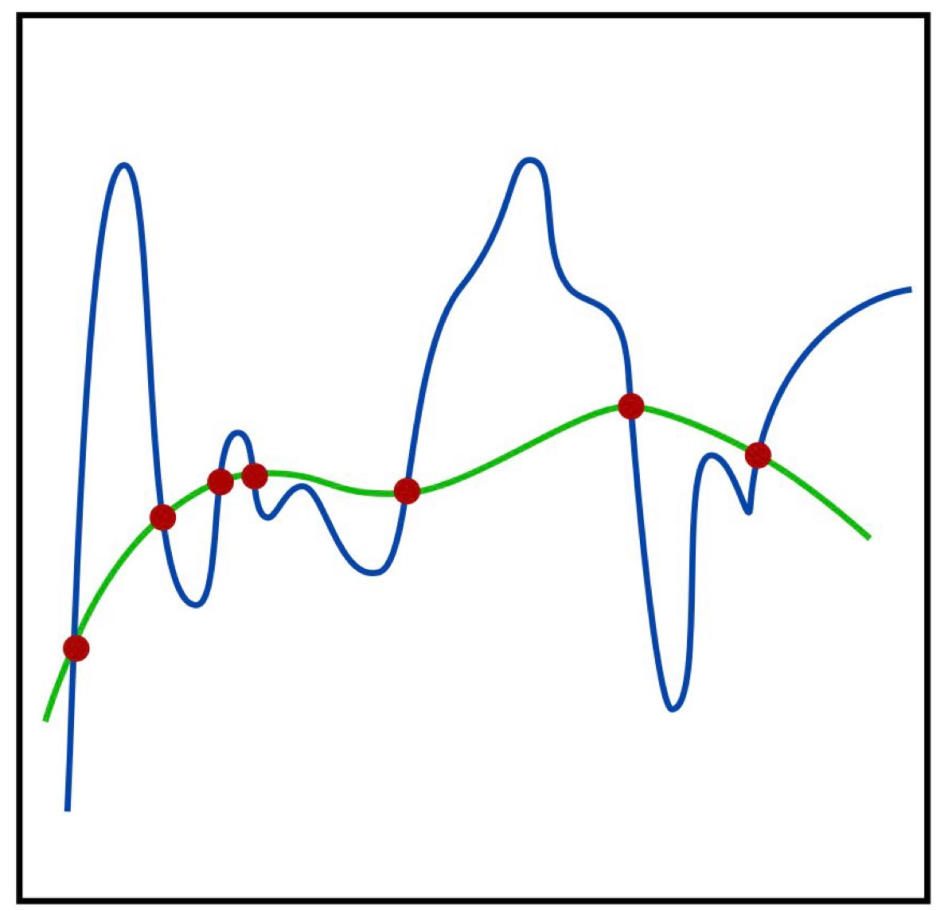
\includegraphics[width=1\linewidth]{./figures/supervised_learning/regularisation_two_plots_zero_test_error.pdf}
    \end{minipage}%
    \hfill
    \begin{minipage}{0.55\linewidth}
        \caption{Motivating regularisation. Two fits, both with 0 test error.}
        \label{fig:regularisation_two_plots}
    \end{minipage}
\end{figure}

The most well known methods of regularisation are L1 and L2 regularisation. Both involve adding a penalty term to the loss function used during training with the intention of encouraging some behaviour in the learning process. There are tons of ways of motivating both L1 and L2 but the most intuitive to me (by a long shot) is a Bayesian approach: assume independence of parameters and impose a prior distribution on them according to whatever bias we hope to bake into the learning process. Then, instead of maximum likelihood estimation, compute
\begin{align*}
    \argmax_{\theta\in\R^{m+1}}\log(p(\theta|D))
    &=
    \argmax_{\theta\in\R^{m+1}}\l[\log(p(D|\theta))+\log(p(\theta))\r]\\
    &=
    \argmin_{\theta\in\R^{m+1}}\l[-\sum_{i=1}^n\log(p(y_i|\x_i,\theta))-\sum_{j=1}^m\log(p(\theta_j))\r].
\end{align*}

\subsubsection{L1 regularisation (LASSO)}
If we would like our to-be-learned parameters to be sparse, then it makes sense to choose a prior which has a lot of mass around 0 and tapers off rather harshly at the tails. A great choice for this is a Laplace prior with mean 0 and variance $2/\lambda$ which yields L1 regularisation. The corresponding density function is given by $p(\theta_j)=\lambda\exp(-2\lambda|\theta_j|)$ and explicit examples are illustrated in \autoref{fig:laplace_pdf}.

\begin{figure}[t]
    \centering
    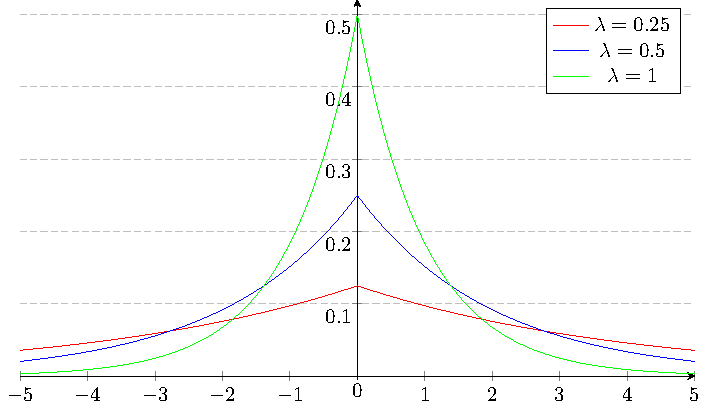
\includegraphics[width=\columnwidth]{./figures/supervised_learning/laplace_pdf.pdf}
    \caption{Laplace pdf with means 0 and decreasing variances according to $\lambda\in\{0.5,1,2,3\}$.}
    \label{fig:laplace_pdf}
\end{figure}

See how as $\lambda$ increases, the variance of the corresponding Laplace distribution decreases and more of the mass becomes centred around 0. The result is that the to-be-learned parameters are further encouraged to flatten out around 0. In line with this, assuming $\theta_1,\dots,\theta_m\overset{\text{i.i.d.}}{\sim}\text{Lap}(0, 2/\lambda)$, the quantity we seek to compute is given by
$$
\argmax_{\theta\in\R^{m+1}}\log(p(\theta|D))
=
\argmin_{\theta\in\R^{m+1}}\l[-\sum_{i=1}^n\log(p(y_i|\x_i,\theta))+\lambda\sum_{j=1}^m|\theta_j|\r].
$$

\subsubsection{L2 regularisation (Ridge)}
If we would like no given parameter to be too large then imposing some sort of MSE penalty on the parameters makes sense. From the Bayesian point of view, this is achieved by imposing a normal prior on the parameters and yields L2 regularisation. That is, if $\theta_1,\dots,\theta_m\overset{\text{i.i.d.}}{\sim}\mathcal{N}(0,\sigma^2)$ then the quantity we seek is
$$
\argmax_{\theta\in\R^{m+1}}\log(p(\theta|D))
=
\argmin_{\theta\in\R^{m+1}}\l[-\sum_{i=1}^n\log(p(y_i|\x_i,\theta))+\lambda\sum_{j=1}^m \theta_j^2\r]
$$
where $\lambda=1/2\sigma^2$.

There's a particularly elegant way to visualise the effects of L1 and L2 reglularisation in terms of how they change the shape of the corresponding loss landscape. It's as if each point in the landscape is sunk according to its distance from the origin and the hyperparameter $\lambda$. The sharpness or curvature of said sinking is prior-dependent: for L1 regularisation it is far sharper, hence the origin acts as more of a sinkhole than in L2 regularisation, inducing sparser minima.

\begin{figure}[t]
    \centering
    \begin{minipage}{0.55\linewidth}
        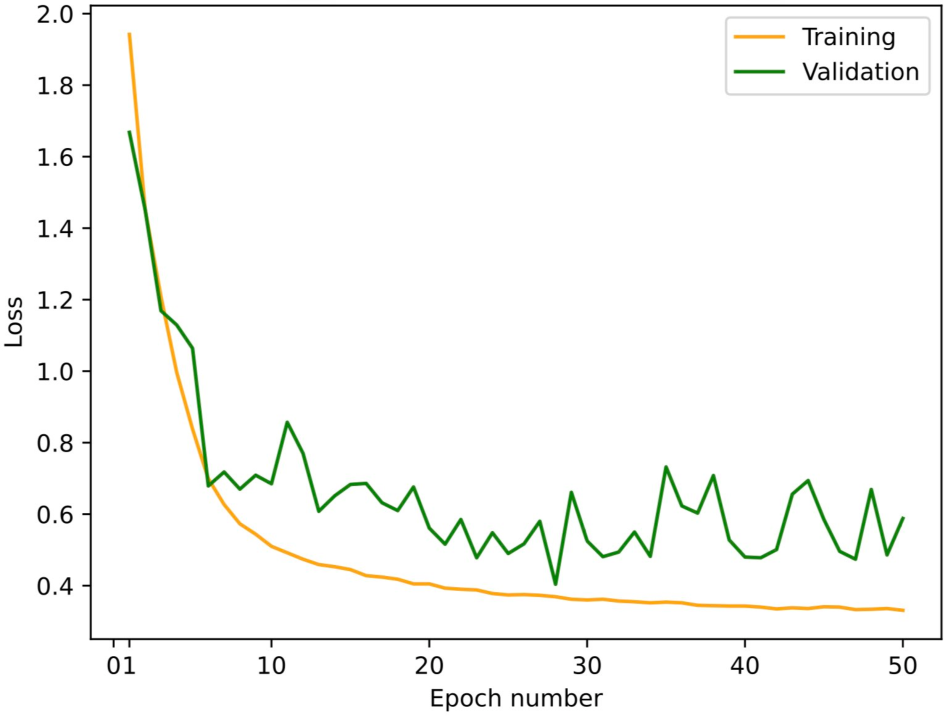
\includegraphics[width=\linewidth]{./figures/neural_nets/REG_early_stopping.pdf}
    \end{minipage}%
    \hfill
    \begin{minipage}{0.44\linewidth}
        \caption{Training and validation losses over 50 epochs. Lowest validation obtained at epoch 28.}
        \label{fig:early_stopping}
    \end{minipage}
\end{figure}

\subsubsection{Early stopping} To motivating early stopping, consider the familiar scenario of training via gradient descent. A natural thought when logging the training loss is whether or not a decrease in training loss from one epoch to the next genuinely pertains to a model that better generalises. How can we be confident that our model isn't simply overfitting the training data if all we see is decrease in training loss?

Early stopping partially alleviates this fear by splitting the training dataset into a smaller training set and a validation set (perhaps 80\%/20\%). After each epoch (or every few), compute both training and validation losses. Said validation loss acts as some measure of the model's ability to generalise. If training loss is decreasing while validation loss is not then the model may be overfitting. As illustration, consider \autoref{fig:early_stopping} in which the training loss continues to decrease in the number of epochs while the validation loss seems to obtain its lowest value around epoch 28.

\subsubsection{Dropout} Dropout is a form of regularisation specific to neural network architectures (I think). Its rough motivation is that we'd prefer not to be overly-reliant on any given subset of neurons at inference time. To prevent such an over-reliance, at the beginning of each epoch, independently set the activation of each neuron to 0 with some probability $p$. This way some portion of neurons are silenced during training for said epoch. As a result, its corresponding parameters are not updated during backpropagation. This idea is illustrated in \autoref{fig:dropout}. Make sure to not apply dropout at ineference time!

\begin{figure}[t]
    \centering
    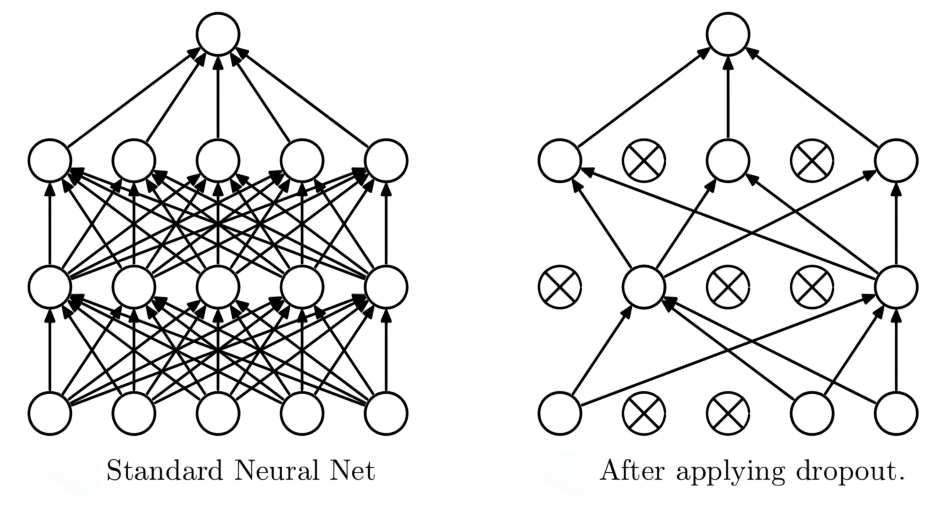
\includegraphics[width=\textwidth]{./figures/neural_nets/REG_dropout.pdf}
    \caption{Dropout.}
    \label{fig:dropout}
\end{figure}

% momentum and adaptive learning rates
\subsection{Momentum + Adaptive Learning Rates}
There are some intuitive ideas which aim to accelerate the gradient descent process. One is momentum, which increases steps made when gradients consistently pointed in the same direction over previous steps. Another is an adaptive learning rate, where each parameter has its own step size that adapts over time to its past gradients.

\subsubsection{Momentum}
Think of a ball rolling downhill: momentum lets it keep moving in the same direction which smoothes out noisy gradients. If gradients keep pointing in the same direction then momentum builds. If gradients oscillate, e.g. traversing like a ravine, then the motion is dampened and momentum is lost.

\begin{figure}[t]
    \centering
    \begin{minipage}{0.62\linewidth}
        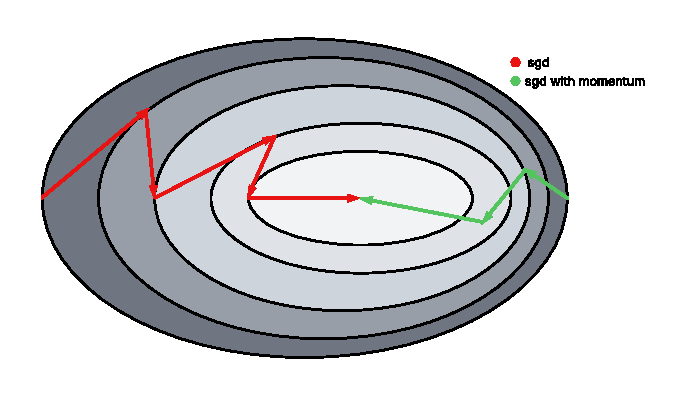
\includegraphics[width=\columnwidth]{./figures/gradient_descent/momentum.pdf}
    \end{minipage}%
    \hfill
    \begin{minipage}{0.38\linewidth}
        \caption{How we might hope convergence would look using momentum.}
        \label{fig:gradient_descent_momentum}
    \end{minipage}
\end{figure}

We impose a momentum-like idea by introducing a velocity vector
$$
\mathbf{v}^{(t+1)}
=
\mu\mathbf{v}^{(t)}-\eta\nabla R_D\l(\theta^{(t)}\r)
$$
with $\mathbf{v}^{(0)}=0$ and change the gradient descent update rule to
$$
\theta^{(t+1)}
=
\theta^{(t)}-\eta\nabla R_D\l(\theta^{(t)}\r)+\mu\mathbf{v}^{(t)}
$$
where $\mu\in[0,1)$ is the momentum coefficient. Typical values include, $\mu\in\{0.9,0.95,0.99\}$. To get a sense of how this refelcts a momentum-like idea, see that
$$
\mathbf{v}^{(1)}
=
-\eta\nabla R_D\l(\theta^{(0)}\r)
$$
and so
$$
\mathbf{v}^{(2)}
=
-\eta\l(\mu\nabla R_D\l(\theta^{(0)}\r)+\nabla R_D\l(\theta^{(1)}\r)\r).
$$
If $\mu\approx1$ and the gradients $\nabla R_D\l(\theta^{(0)}\r)\approx\nabla R_D\l(\theta^{(1)}\r)$ then $\mathbf{v}^{(2)}$ will confidently boost $\theta^{(3)}$ in the direction of the first two gradients. If $\nabla R_D\l(\theta^{(0)}\r)\approx-\nabla R_D\l(\theta^{(1)}\r)$ then, as intuition would suggest, $\mathbf{v}^{(2)}=0$.

\subsubsection{Adaptive learning rates}
Why have a fixed learning rate? Why have the same learning rate for each parameter? Adaptive learning rates aim to alleviate the oversimplications these questions pertain to. For some intuition as to how learning rates might change: if up to the $t^{\text{th}}$ optimisation step the gradients for a given parameter have been large then it has presumably converged decently so its learning rate would ideally get smaller. AdaGrad does this is by storing a per parameter running total of gradients, as in
$$
G_i^{(t)}
=
\sum_{\tau=1}^t\l(\nabla_{\theta_i}R_D(\theta_i^{(\tau)})\r)^2
$$
and switching the optimisation step to
$$
\theta_i^{(t+1)}
=
\theta_i^{(t)}-\eta_i\nabla_{\theta_i}^{(t)}R_D(\theta_i^{(t)})
$$
where $\eta_i^{(t)}=\frac{\eta}{\sqrt{G_i^{(t)}}+\epsilon}$ is the $i^{\text{th}}$ parameter's learning rate at step $t$. There are more elaborate adaptive learning rate methods than this, e.g. RMSProp and Adam, but AdaGrad conveys the idea sufficiently well.

% hyperparam tuning
\subsection{Hyperparameter Tuning}
Hyperparameters are the tunable parts of an architecture which are not learned during training. Bad hyperparameters will yield training issues like divergence, overfitting or underfitting. A simple example of a hyperparameter I can think of is the learning rate in vanilla gradient descent. Some choices of learning rate will result in better generalisation than other choices. For a more sophisticated example, consider architecture-related hyperparameters, e.g. the number of hidden layers in a multi-layer perceptron.

\subsubsection{Random search}
Begin by designating some portion of the training data for validation (maybe 80\% training, 20\% validation). 

Each hyperparameter may take on a set of values, i.e. the $m$ hyperparameters $h_1,\dots,h_m$ induce the samples spaces $\Omega_{h_1},\dots,\Omega_{h_m}$ and the grid of all possible hyperparameter configurations is thus $\Omega_1\times\dots\times\Omega_m$. In a perfect world, you'd be able to train a model for each hyperparameter configuration and choose whichever yields the lowest validation loss. We don't live in a perfect world and the cardinality of said grid is often too large. In line with this, instead of traversing it entirely, uniformly randomly sample from it a number of times and train with said hyperparameter configuration. Choose whichever configuration yielded the lowest validation loss.

\subsubsection{$k-$fold cross-validation}
For a better idea of how a configuration of hyperparameters will help generalise post-training, consider partitioning the training data into $k$ disjoint subsets (or folds) $D_1,\dots,D_k$. Then, for $i=1,\dots,k$, train on $D\backslash D_i$ and validate on $D_i$. Take the mean of the $k$ validation losses. Choose whichever hyperparameter configuration yields the lowest mean validation loss.

\subsubsection{Honourable mention: benchmark overfitting}
Suppose research groups A and B independently publish results on nearly identical single hidden layer MLPs for the same task. The only difference is the number of neurons in the hidden layer — 99 for A, 100 for B. Their training setup is otherwise identical: same data, same splits, same optimisation. Group A's model achieves lower test error, and so a company adopts their architecture. How is this fundamentally different from a single group training both 99- and 100-neuron models and then choosing based on test loss? More broadly, how is it different from tuning hyperparameters directly on the test set?

In both cases, the test error becomes a biased (optimistic) estimate of generalisation. If this process repeats across the community, the field as a whole is implicitly tuning to the test set. This phenomenon is called benchmark overfitting, and it underlines the need for practices like shuffling data in the pipeline and, more importantly, evolving benchmarks over time.

% neural nets
\section{Neural Networks}
It's often the case that someone's intended meaning when stating `neural networks' is more precisely multi-layer perceptrons (MLPs), perhaps the simplest class of neural networks beyond single-layer perceptrons. Rigorously formulating MLPs is one of those things that's useful to do at least once; consistent notation is 90\% of the effort.

% neural networks
\subsection{Multi-Layer Perceptrons (MLPs)}
\label{sec:multi_layer_perceptrons}

Multi-layer perceptrons (MLPs) are fully-connected feed-forward networks consisting of an input layer (where data is input), hidden layers and an output layer. An MLP with three hidden layers is illustrated in \autoref{fig:MLP}. Each layer is made up of a number of neurons, each of which has a real-valued activation value.  For any neuron in a non-input layer, its activation value is the output of a non-linear activation function given, as input, the neuron's real-valued bias plus a weighted sum of the activation values of the neurons in its preceding layer. Regarding their inspiration from the human brain, consider this footnote\footnote{\url{https://stats.stackexchange.com/a/159172}}.

The application of MLPs to learning functions from data is due to their expressivity, expressive-efficiency and tractability. Their expressivity is known due to a proof of their universal function approximation by Cybenko. To add to this, their high expressive-efficiency has been demonstrated empirically and ensures that the number of model components (hidden layers and neurons) needed to represent arbitrary functions is far lower than competing model classes. As for their tractability, MLPs allow for an evaluation of the approximation of the function of interest with complexity quadratic in the number of neurons of each layer of the MLP (after the heavy simplifcation of assuming a roughly equal number of neurons in each layer).

\begin{figure}[t]
    \centering
    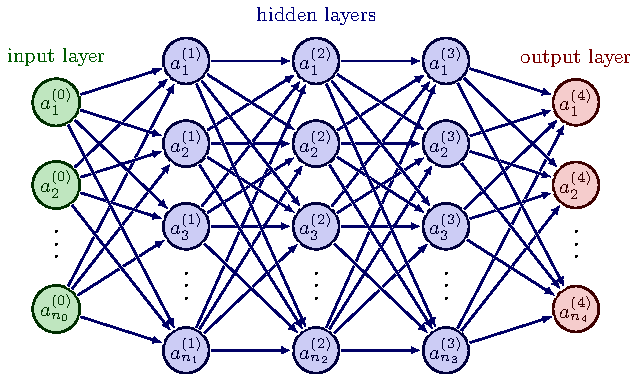
\includegraphics[width=\linewidth]{./figures/neural_nets/MLP_1.pdf}
    \caption{A multi-layer perceptron (MLP) with $k=3$ hidden layers.}
    \label{fig:MLP}
\end{figure}

For brevity, given $m,n\in\mathbb{N}$ with $m\leq n$ let $[n]_m=\{m,\dots,n\}$ and let $[n]=[n]_1$. For further ease of notation, given an MLP with $k$ hidden layers, denote the index of the input layer by $0$, the output layer by $k+1$ and by extension the $j^{\text{th}}$ layer by $j\in[k+1]_0$. Additionally, consider the following denotations
\begin{itemize}
    \item[--] $n_j\in\mathbb{Z}_{\geq1}$ is the number of neurons in layer $j$.
    \item[--] $a_i^{(j)}\in\mathbb{R}$ is the activation value of neuron $i$ in layer $j$.
    \item[--] $w_{i,l}^{(j)}\in\mathbb{R}$ is the weight associated with the edge to neuron $i$ in layer $j\in[k+1]$ from neuron $l$ in the previous layer.
    \item[--] $b_i^{(j)}\in\mathbb{R}$ is the bias of neuron $i$ in layer $j\in[k+1]$.
    \item[--] $\sigma_j:\mathbb{R}\rightarrow\mathbb{R}$ is the non-linear activation function of layer $j\in[k+1]$.
\end{itemize}
From here we can express the activation value of any neuron in a non-input layer in terms of the activation values of the neurons in the layer which precedes it as
\begin{align*}
    a_i^{(j+1)}
    &=
    \sigma_{j+1}\l(
    \sum_{l=1}^{n_j} w_{i,l}^{(j+1)}a_l^{(j)} + b_i^{(j+1)}
    \r)\\
    &=
    \sigma_{j+1}\l(
    \l[w_{i,1}^{(j+1)} \dots w_{i,n_j}^{(j+1)}\r]
    \begin{bmatrix}
        a_1^{(j)}\\
        \vdots\\
        a_{n_j}^{(j)}
    \end{bmatrix}
    +
    b_i^{(j+1)}
\r)
\end{align*}
for $j\in[k]_0$. The reason for writing the second equality above, involving the dot product of two vectors, is that it helps us to see how using matrix-vector notation allows us to write an elegant and compact expression for the activation values of all neurons in a non-input layer in terms of the activation values of the neurons belonging to its preceding layer as
$$
\begin{bmatrix}
    a_1^{(j+1)}\\
    \vdots\\
    a_{n_{j+1}}^{(j+1)}
\end{bmatrix}
=
\sigma_{j+1}\l(
\begin{bmatrix}
    w_{1,1}^{(j+1)} & \dots & w_{1,n_j}^{(j+1)}\\
    \vdots & \ddots & \vdots\\
    w_{n_{j+1},1}^{(j+1)} & \dots & w_{n_{j+1},n_j}^{(j+1)}
\end{bmatrix}
\begin{bmatrix}
    a_1^{(j)}\\
    \vdots\\
    a_{n_j}^{(j)}
\end{bmatrix}
+
\begin{bmatrix}
    b_1^{(j+1)}\\
    \vdots\\
    b_{n_{j+1}}^{(j+1)}
\end{bmatrix}
\r)
$$
which we abbreviate to
$$
\mathbf{a}^{(j+1)}=\sigma_{j+1}\l(\mathbf{W}^{(j+1)}\mathbf{a}^{(j)}+\mathbf{b}^{(j+1)}\r)
$$
where the activation function $\sigma_{j+1}$ is applied element-wise.

If we fix the structure and choice of activation functions of an MLP then all that is left to learn are its weights and biases. This is often done using gradient descent to minimise some loss function in which gradients are computed via back-propagation. Such a loss function can be a principled measure, e.g. corresponding to maximum likelihood, but this is not always necessary: ad-hoc loss functions are sometimes employed.

\begin{tcolorbox}[title={\centering\textbf{Crudely advocating for depth over width}}, colback=myLightBlue, colbacktitle=myDarkBlue, colframe=myDarkBlue, coltitle=white]
    The complexity of a forward pass of an MLP can be expressed in terms of the number of neurons in each layer as
    $$
    \mathcal{O}
    \l(
    \sum_{j=1}^{k+1}n_{j-1}\cdot n_j
    \r).
    $$
    Very crudely supposing $n_0=\dots=n_{k+1}=n$ yields a complexity of
    $
    \mathcal{O}((k+1)n^2)
    $
    which grows linearly in the number of layers and quadratically in the number of neurons per layer.
\end{tcolorbox}

% \subsubsection{Example}

\begin{figure}[t]
    \centering
    \begin{minipage}{0.59\linewidth}
        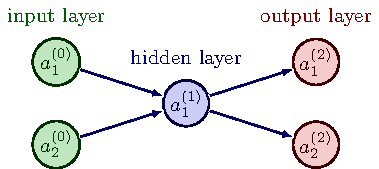
\includegraphics[width=1\textwidth]{./figures/neural_nets/MLP_2.pdf}
    \end{minipage}%
    \hfill
    \begin{minipage}{0.4\linewidth}
        \caption{A neural network with one hidden layer ($k=1$).}
        \label{fig:neural_nets_simple_example}
    \end{minipage}
\end{figure}

\begin{example}
    Consider the neural network in \autoref{fig:neural_nets_simple_example} whose input, hidden and output layers consist of two, one and two neurons respectively. With such a simple neural network, we may explicitly express the output neurons $a_1^{(2)}$ and $a_2^{(2)}$ in terms of the input neurons $a_1^{(0)}$ and $a_2^{(0)}$. We see that $n_0=2$, $n_1=1$ and $n_2=2$ and so
    $\mathbf{W}^{(1)}=
    \begin{bmatrix}
        w_{1,1}^{(1)} & w_{1,2}^{(1)}
    \end{bmatrix}
    $
    and
    $\mathbf{W}^{(2)}=
    \begin{bmatrix}
        w_{1,1}^{(2)}\\
        w_{2,1}^{(2)}
    \end{bmatrix}.
    $
    Noting additionally that $\mathbf{b}^{(1)}=b_1^{(1)}$ and
    $\mathbf{b}^{(2)}=
    \begin{bmatrix}
        b_{1}^{(2)}\\
        b_{2}^{(2)}
    \end{bmatrix}$
    we can explicitly express the activation of the single neuron in the hidden layer as
    \begin{align*}
    \mathbf{a}^{(1)}
    &=
    \sigma_1\l(\mathbf{W}^{(1)}\mathbf{a}^{(0)}+\mathbf{b}^{(1)}\r)\\
    &=
    \sigma_1\l(w_{1,1}^{(1)}a_1^{(0)}+w_{1,2}^{(1)}a_2^{(0)}+b_1^{(1)}\r)
    \end{align*}
    which is just the scalar value $a_1^{(1)}$. For the output layer, we have
    \begin{align*}
    \mathbf{a}^{(2)}
    &=
    \sigma_2\l(\mathbf{W}^{(2)}\mathbf{a}^{(1)}+\mathbf{b}^{(2)}\r)\\
    &=
    \sigma_2\l(
    \begin{bmatrix}
        w_{1,1}^{(2)}a_1^{(1)} + b_1^{(2)}\\
        w_{2,1}^{(2)}a_1^{(1)} + b_2^{(2)}
    \end{bmatrix}
    \r)\\
    &=
    \sigma_2\l(
    \begin{bmatrix}
        w_{1,1}^{(2)}\sigma_1\l(w_{1,1}^{(1)}a_1^{(0)}+w_{1,2}^{(1)}a_2^{(0)}+b_1^{(1)}\r) + b_1^{(2)}\\
        w_{2,1}^{(2)}\sigma_1\l(w_{1,1}^{(1)}a_1^{(0)}+w_{1,2}^{(1)}a_2^{(0)}+b_1^{(1)}\r) + b_2^{(2)}
    \end{bmatrix}
    \r)\\
    &=
    \begin{bmatrix}
        \sigma_2\l(w_{1,1}^{(2)}\sigma_1\l(w_{1,1}^{(1)}a_1^{(0)}+w_{1,2}^{(1)}a_2^{(0)}+b_1^{(1)}\r) + b_1^{(2)}\r)\\
        \sigma_2\l(w_{2,1}^{(2)}\sigma_1\l(w_{1,1}^{(1)}a_1^{(0)}+w_{1,2}^{(1)}a_2^{(0)}+b_1^{(1)}\r) + b_2^{(2)}\r)
    \end{bmatrix}.
    \end{align*}
    As such, the activations of the output neurons are given by
    \begin{align*}
        a_1^{(2)}&=\sigma_2\l(w_{1,1}^{(2)}\sigma_1\l(w_{1,1}^{(1)}a_1^{(0)}+w_{1,2}^{(1)}a_2^{(0)}+b_1^{(1)}\r) + b_1^{(2)}\r)\\
        a_2^{(2)}&=\sigma_2\l(w_{2,1}^{(2)}\sigma_1\l(w_{1,1}^{(1)}a_1^{(0)}+w_{1,2}^{(1)}a_2^{(0)}+b_1^{(1)}\r) + b_2^{(2)}\r).
    \end{align*}
\end{example}

\begin{tcolorbox}[title={\centering\textbf{Further crudely advocating for depth over width}}, colback=myLightBlue, colbacktitle=myDarkBlue, colframe=myDarkBlue, coltitle=white]
    A perhaps more important result is how, geometrically, MLPs split the input space into a bunch of regions. It turns out that the number of regions by which a single-hidden layer MLP with two input neurons and $n$ neurons in its hidden layer splits the space is bounded above by $\frac{1}{2}(n^2+n+2)$ which is quadratic in $n$. For an MLP with $k$ hidden layers of $n$ neurons each, the number of regions by which the space is split is bounded above by
    $$
    \frac{1}{2}(n^2+n+2)\l(\frac{n}{n_0}+1\r)^{n_0(k-1)}
    $$
    which is exponential in $k$. Again, we argue for increasing depth $k$ over width $n$. A natural quesiton is to what extent these bounds are tight in practice.
\end{tcolorbox}

% universal function approximation theorem
\subsubsection{Universal Function Approximation with MLPs}
\label{subsubsec:universal_function_approximation_theorem}
A class of functions, or function class, $\mathcal{F}_S$ is capable of universal function approximation on $S\subset\R^m$ compact (closed and bounded) if for all continuous $f:S\to\R$ and $\epsilon>0$ there exists some $\hat{f}\in\mathcal{F}_S$ such that
$$
\max_{x\in S}\l|f(x)-\hat{f}(x)\r|<\epsilon.
$$
Note that such a function family can be used to approximate functions whose codomain is $\R^m$ by performing coordinate-wise approximation. 

The family of polynomials is capable of universal function approximation as shown by Weierstrass in 1885. A directly equivalent statement to a function class satisfying the universal function approximation is the function ckass being dense in $C(S)$ with respect to the supremum norm. Here, $C(S)$ denotes the set of all continuous real-valued functions with compact domain $S\subset\R^m$. Quick note: usually the domain of the to-be-approximated function is denoted by $K$ but I denote the number of layers in an MLP using a $k$ so I'd like to avoid the confusion by using $S$ instead. Instead of offering a rigorous proof, I'll motivate the overall idea in three steps starting with a simpler case: functions of the form $f:S\to\R$ where $S\subset\mathbb{N}$ with $\#S<\infty$.

\subsubsection*{Step 1: Motivating the idea for $S$ finite}
Without loss of generality, let $S=[\#S]$. We seek to show that for all $\epsilon>0$ there exists an MLP with one hidden layer and one node in its output layer, whose output is denoted by $\hat{f}(x)$, which satisfies
$$
\max_{x\in [\#S]}\l|f(x)-\hat{f}(x)\r|<\epsilon.
$$
First note that for all $x\in[\#S]$,
\begin{align*}
f(x)
&=
\sum_{s=1}^{\#S}f(x)\mathbbm{1}(x=s)\\
&=
\sum_{s=1}^{\#S}f(x)(\mathbbm{1}(x\geq s)-\mathbbm{1}(x\geq s+1))
\end{align*}
so we already see that a single neuron in the ouput layer of a single hidden layer MLP ($2\cdot\#S$ neurons in hidden layer) with weights
$$
\mathbf{W}^{(2)}
=
\begin{bmatrix}
    f(1) & -f(1) & \dots & f(\#S) & -f(\#S)
\end{bmatrix},
$$
i.e. $w_{1,s}^{(2)}=(-1)^{s+1}f\l(\l\lfloor\frac{s+1}{2}\r\rfloor\r)$, and bias $\mathbf{b}^{(2)}=0$ is sufficient if the $2\cdot\#S$ neurons in the hidden layer approximate
$$
\mathbbm{1}(x\geq1),\mathbbm{1}(x\geq2),\mathbbm{1}(x\geq2),\mathbbm{1}(x\geq3),\dots,\mathbbm{1}(x\geq\#S),\mathbbm{1}(x\geq\#S+1)
$$
with the absolute error of each approximation bounded by $\epsilon$. Note that the final indicator $\mathbbm{1}(x\geq\#S+1)$ is redundant so you only really need $2\cdot\#S-1$ neurons but I'll keep it for the nicer number. Also note that these are just renditions of the Heaviside function but I prefer sticking with the indicator function notation. This exact idea can be realised elegantly using the sigmoid as activation for the hidden layer. To see this, note that
\begin{align*}
    \sigma\l(10^{\#S}(x-n)+10^{\#S-9}\r)
    &=
    \frac{1}{1+\exp\l(-10^{\#S}(x-n)+10^{\#S-9}\r)}\\
    &=
    \frac{1}{1+\exp\l(n-x+10^{-9}\r)^{10^{\#S}}}
\end{align*}
approximates the Heaviside function $H(x-n)$ with some small leakage. To hit certain levels of precision, i.e. attaining the desired $\epsilon$ bound, simply decrease the exponent in which $-9$ currently lies. You can probably express the exponent in terms of $\epsilon$ explicitly (maybe $\epsilon^{-1}$) but the idea is the point here. So what we want is for the $\l\lceil\frac{s+1}{2}\r\rceil^{\text{th}}$ neuron in the hidden layer to approximate $H\l(x-\l\lceil\frac{s+1}{2}\r\rceil\r)$ for $s\in[\#S]$. This is straightforward using a sigmoid activation function in the hidden layer given the approximation above. Simply set the weights and biases accordingly: $w_{s,1}^{(1)}=10^{\#S}$ and $b_s^{(1)}=-10^{\#S}\l(\l\lceil\frac{s+1}{2}\r\rceil-10^{-9}\r)$ and we're done.

\subsubsection*{Step 2: Extending the idea to $S\subset\R$ compact}
If $f\in C(S)$ for $S\subset\R$ compact then $f$ is uniformly continuous and so for all $\epsilon>0$ there exists $\delta>0$ such that
$$
|x-y|<\delta\implies|f(x)-f(y)|<\epsilon.
$$
Note that if we have a Lipschitz constant $L$ for a given $f$ then $\delta=\epsilon/L$ suffices. The reason this $\epsilon-\delta$ statement is useful is that if we split $S$ into $N$ subintervals whose width is bounded by $\delta$ then for all $c,x$ within the same subinterval we have
$$
\l|f(x)-f(c)\r|<\epsilon.
$$
To realise this idea, if $S=[a,b]$ then split $S$ according to
$$
a=x_0<x_1<\dots<x_N=b
$$
such that $x_{i+1}-x_i<\delta$ and take $c=(x_i+x_{i+1})/2$, the midpoint of $[x_i,x_{i+1}]$. The number of subintervals $N$ needed depends on $a,b$ and $\delta$, e.g. $N=\l\lceil\frac{b-a}{\delta/2}\r\rceil$ works but the denominator just needs to be less than $\delta$ so $\delta/1.1$ would give a tighter $N$. From this we see that
$$
N
\approx
\frac{b-a}{\delta}
=
\frac{L(b-a)}{\epsilon}.
$$
The higher we take $N$ the more accurate of an approximation we get. This idea of splitting $S$ into $N$ intervals is nice because it requires us to approximate only one point $c_i=(x_i+x_{i+1})/2$ on each subinterval, i.e. we are back to the simpler case which started our motivation of approximating at a fixed number of points.

With this idea in mind, the number of required neurons to realise our idea
$$
2N
=
2\frac{L(b-a)}{\epsilon}
$$
grows linearly in $L$, the interval length $b-a$ and the reciprocal of the desired level of precision $1/\epsilon$. In practice, you only have control of the desired level of precision $\epsilon$.

\subsubsection*{Step 3: Extending the idea to $S\subset\R^m$ compact}
The idea is really not very different. Imagine $S\subset\R^2$ compact. The compactness is very hepful for visualisation. As long as we can create indicator-approximate functions on separate regions of $S$ then use exactly the idea described above: split $S$ into separate regions and approximate $f$ on a single point in each. To see that we can approximate the indicator on regions of $S\subset\R^2$ simply see that we can create wall-like objects using the same idea of creating a 'steep' plane and sigmoiding it. As such, to isolate some region, produce three walls which enclose a region and you're done. If you want a more accurate enclosing of the region then use more walls. Without boundedness, which is given by compactness, this idea wouldn't work. Extend this idea to $\R^m$ and voilà.


\subsubsection*{Is the idea used here practical?}
What the idea conveyed shows is \textit{that} (and even \textit{how}) an MLP can approximate any function in $C(S)$ for $S\subset\R^m$ compact. It is not at all an indicator of how MLPs learned via gradient descent, in practice, go about approximating functions from data.

An interesting addition to this note is how this formulation gives an idea of how the weights from the hidden layer to the output explicitly encode the evaluation of the to-be-approximated function. Again, this is not what we'd expect MLPs to do in practice, instead they find a much more efficient representation, sharing information between neurons. Reminds me a lot of the research 3Blue1Brown discussed in one of his videos about transfromers and LLMs in which we spoke about how the LLM `knows' to assign a high probability to the token \texttt{Jordan} when given \texttt{My favourite basketballer is Michael} as input. How does it `know' to do that? It isn't at all implied by the grammar/semantics/whatever of the sentence. Said research concluded things about such pieces of knowledge being stored in the weights of the MLPs of the transformer blocks.

\subsubsection{Posing classification as a regression problem}
Which space does one transform their samples into in order to linearly separate them? In the case of neural net approaches, for $K-$classification, it's the $(K-1)$-probability simplex given by
$$
\l\{(x_1,\dots,x_K)\in[0,1]^K|x_1+\dots+x_K=1\r\}.
$$
The $2-$probability simpelx coloured according to argmax is illustrated in \autoref{fig:2_prob_simplex}.
\begin{figure}[t]
    \centering
    \begin{minipage}{0.52\linewidth}
        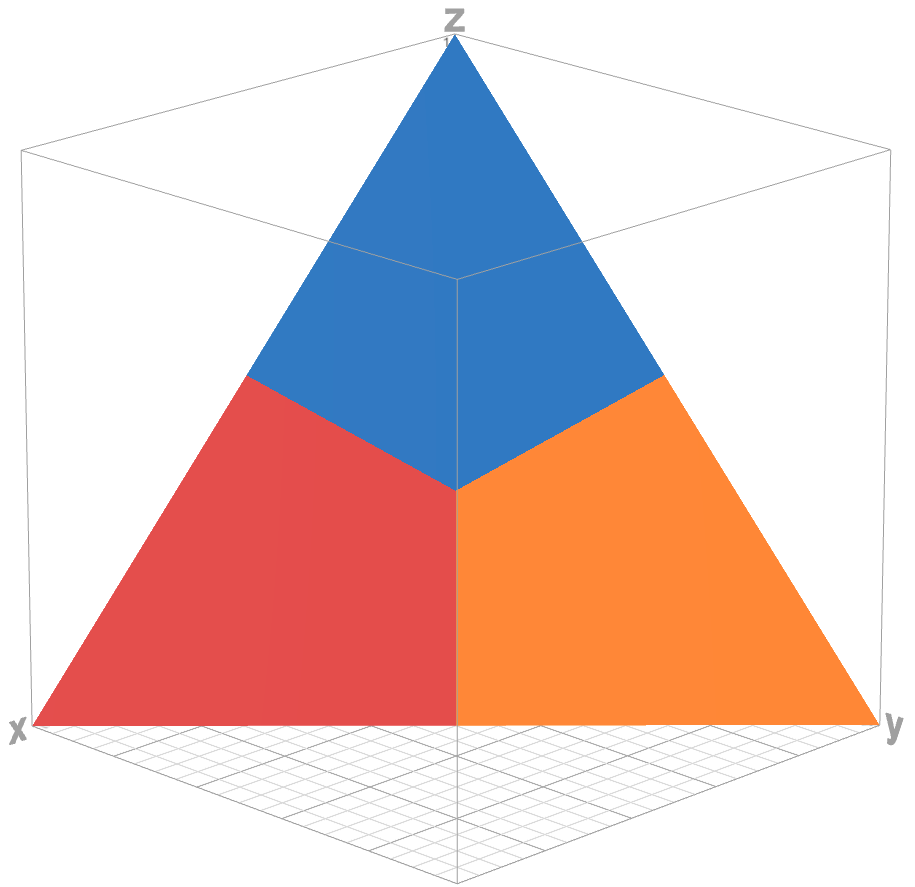
\includegraphics[width=1\textwidth]{./figures/neural_nets/MLP_simplex_argmax.png}
    \end{minipage}%
    \hfill
    \begin{minipage}{0.48\linewidth}
        \caption{The $2-$probability simplex coloured according to argmax in the three coordinates.}
        \label{fig:2_prob_simplex}
    \end{minipage}
\end{figure}
From the figure, it is clear how argmax can be computed by splitting the $2$-probability simplex via two planes, e.g. the intersection of $x>y$ and $x>z$ on the simplex yield the red region. As such, neural nets used for classification can be seen as performing regression on the $2-$probability simplex.

% backprop
\subsection{Backpropagation for MLPs}
\label{subsec:backprop}

Backpropagation is a method of computing the gradient of a loss function pertaining to an MLP (or more generally some neural network) with respect to its weights and biases. Said gradients are used to learn suitable MLP parameters via gradient descent. We'll soon see why it's called backpropagation: it computes the gradients of interest in a way that requires going forwards through the MLP and then backwards. As with formulating MLPs, it's good to rigorously derive backpropagation at least once. It's sort of strange that I haven't done that yet (August 2025 is time of writing) and have just trusted that it holds up.

Onto the derivation, which makes use of the notation introduced earlier. Recall that a loss function is of the form
$$
\mathcal{L}:\Omega_{Y}\times\Omega_{Y}\to\R_{\geq0}
$$
and that the loss induced by a choice of model parameters $\theta$ for a sample $(\x,y)$, which we will henceforth crudely denote by $\mathcal{L}$, is given by
$$
\mathcal{L}\l(y,f_{\theta}(\x)\r),
$$
where $f_{\theta}$ is the model itself. Note that taking the gradient of $\mathcal{L}(y,f_{\theta}(\x))$ with respect to $\theta$ is perfectly valid even though the function $\mathcal{L}$ itself is not a function of $\theta$. For an MLP,
$$
\theta
=
\l(\mathbf{W}^{(1)},\dots,\mathbf{W}^{(k+1)},\mathbf{b}^{(1)},\dots,\mathbf{b}^{(k+1)}\r).
$$
Let $\mathbf{z}^{(j)}=\mathbf{W}^{(j)}\mathbf{a}^{(j-1)}+\mathbf{b}^{(j)}$ for $j\in[k+1]$ from which we have $\mathbf{a}^{(j)}=\sigma_{j}\l(\mathbf{z}^{(j)}\r)$. Further, let
$$
\delta^{(j)}_i
=
\frac{\partial\mathcal{L}}{\partial z^{(j)}_i}
$$
for $j\in[k+1]$ and $i\in[n_j]$ where $\l(z_1^{(j)},\dots,z_{n_j}^{(j)}\r)=\mathbf{z}^{(j)}$. We seek to derive four statements:
\begin{enumerate}
    \item $\delta_i^{(k+1)}=\sigma_{k+1}'\l(z_i^{(k+1)}\r)\frac{\partial\mathcal{L}}{\partial a_i^{(k+1)}}$ for $i\in[k+1]$
    \item $\delta_i^{(j)}=\sigma_{j}'\l(z_i^{(j)}\r)\l(\l(\mathbf{W}^{(j+1)}\r)^\top\delta^{(j+1)}\r)_i$ for $j\in[k]$ and $i\in[n_j]$
    \item $\frac{\partial\mathcal{L}}{\partial b^{(j)}_i}=\delta^{(j)}_i$ for $j\in[k+1]$ and $i\in[n_j]$
    \item $\frac{\partial\mathcal{L}}{\partial w_{l,i}^{(j)}}=\delta_l^{(j)}a_i^{(j-1)}$ for $j\in[k+1]$, $i\in[n_{j-1}]$ and $l\in[n_j]$
\end{enumerate}
Before deriving each statement in order, we can see already what was meant earlier by propagating backwards through the MLP: to compute the gradients relevant to performing gradient descent, backpropagation requires the computation of $\mathbf{z}^{(1)},\dots,\mathbf{z}^{(k+1)}$ from which $\delta^{(k+1)}$ can be computed. Note that the $\frac{\partial\mathcal{L}}{\partial a_i^{(k+1)}}$ term in the first statement is often easily computed, e.g. for MSE loss we have
$$
\frac{\partial\mathcal{L}}{\partial a_i^{(k+1)}}
=
a_i^{(k+1)}-y_i.
$$
From there, one can compute $\delta^{(k)},\dots,\delta^{(1)}$ in that order, effectively propagating through the MLP backwards. With $\delta^{(1)},\dots,\delta^{(k+1)}$ and $\mathbf{a}^{(0)},\mathbf{a}^{(1)}=\sigma_1\l(\mathbf{z}^{(1)}\r),\dots,\mathbf{a}^{(k+1)}=\sigma_{k+1}\l(\mathbf{z}^{(k+1)}\r)$, computing the relevant gradients is straightforward.

\vspace{10pt}
\noindent\textbf{Statement 1.} Using the chain rule, see that
\begin{align*}
    \delta_i^{(k+1)}
    &=
    \frac{\partial\mathcal{L}}{\partial z_i^{(k+1)}}\\
    &=
    \frac{\partial\mathcal{L}}{\partial a_i^{(k+1)}}\frac{a_i^{(k+1)}}{\partial z_i^{(k+1)}}\\
    &=
    \sigma_{k+1}'\l(z_i^{(k+1)}\r)\frac{\partial\mathcal{L}}{\partial a_i^{(k+1)}}.
\end{align*}

\noindent\textbf{Statement 2.} First, note that
\begin{align*}
    \l(\mathbf{W}^{(j+1)}\r)^\top\delta^{(j+1)}
    &=
    \begin{bmatrix}
        w_{1,1}^{(j+1)}   & \dots  & w_{n_{j+1},1}^{(j+1)}\\
        \vdots            & \ddots & \vdots               \\
        w_{1,n_j}^{(j+1)} & \dots  & w_{n_{j+1},n_j}^{(j+1)}
    \end{bmatrix}
    \begin{bmatrix}
        \delta_1^{(j+1)}\\
        \vdots\\
        \delta_{n_{j+1}}^{(j+1)}
    \end{bmatrix}\\
    &=
    \sum_{l=1}^{n_{j+1}}\delta_l^{(j+1)}
    \begin{bmatrix}
        w_{l,1}^{(j+1)}\\
        \vdots\\
        w_{l,n_j}^{(j+1)}
    \end{bmatrix}
\end{align*}
and so
$$
\l(\l(\mathbf{W}^{(j+1)}\r)^\top\delta^{(j+1)}\r)_i
=
\sum_{l=1}^{n_{j+1}}\delta_l^{(j+1)}w_{l,i}^{(j+1)}
$$
which reduces the to-be-derived statement to
$$
\delta_i^{(j)}
=
\sigma_j'(z_i^{(j)})\sum_{l=1}^{n_{j+1}}\delta_l^{(j+1)}w_{l,i}^{(j+1)}.
$$
Using the chain rule, we deduce that
\begin{equation*}
    \label{eq:back_prop_statement_2}
    \delta_i^{(j)}
    =
    \frac{\partial\mathcal{L}}{\partial z_i^{(j)}}
    =
    \sum_{l=1}^{n_{j+1}}\frac{\partial\mathcal{L}}{\partial z_l^{(j+1)}}\frac{\partial z_l^{(j+1)}}{\partial z_i^{(j)}}
    =
    \sum_{l=1}^{n_{j+1}}\delta_l^{(j+1)}\frac{\partial z_l^{(j+1)}}{\partial z_i^{(j)}}.
\end{equation*}
To complete our deduction, see that
$$
z_l^{(j+1)}
=
\sum_{i=1}^{n_j}w_{l,i}^{(j+1)}\sigma_{j+1}\l(z_i^{(j)}\r)+b_l^{(j+1)}
$$
from which we obtain
$$
\frac{\partial z_l^{(j+1)}}{\partial z_i^{(j)}}
=
\sigma_{j+1}'(z_i^{(j)})w_{l,i}^{(j+1)}
$$
completing the deduction.

\vspace{10pt}
\noindent\textbf{Statement 3.} This one's a simple application of the chain rule, as in
$$
\frac{\partial\mathcal{L}}{\partial b_i^{(j)}}
=
\sum_{l=1}^{n_{j+1}}\frac{\partial\mathcal{L}}{\partial z_l^{(j)}}\frac{\partial z_l^{(j)}}{\partial b_i^{(j)}}
=
\frac{\partial\mathcal{L}}{\partial z_i^{(j)}}
=
\delta_i^{(j)}.
$$
\textbf{Statement 4.} As before, see that
$$
z_l^{(j)}
=
\sum_{i=1}^{n_j}w_{l,i}^{(j)}a_i^{(j-1)}+b_l^{(j)}
$$
which yields
$$
\frac{\partial z_l^{(j)}}{\partial w_{l,i}^{(j)}}
=
a_i^{(j-1)}.
$$
To complete the derivation, consider
$$
\frac{\partial\mathcal{L}}{\partial w_{l,i}^{(j)}}
=
\frac{\partial\mathcal{L}}{\partial z_l^{(j)}}\frac{\partial z_l^{(j)}}{\partial w_{l,i}^{(j)}}
=
\delta_l^{(j)}a_i^{(j-1)}.
$$

% convolutional neural networks
\subsection{Convolutional Neural Networks (CNNs)}
\label{subsec:conv_neural_networks}

\begin{figure}[t]
    \centering
    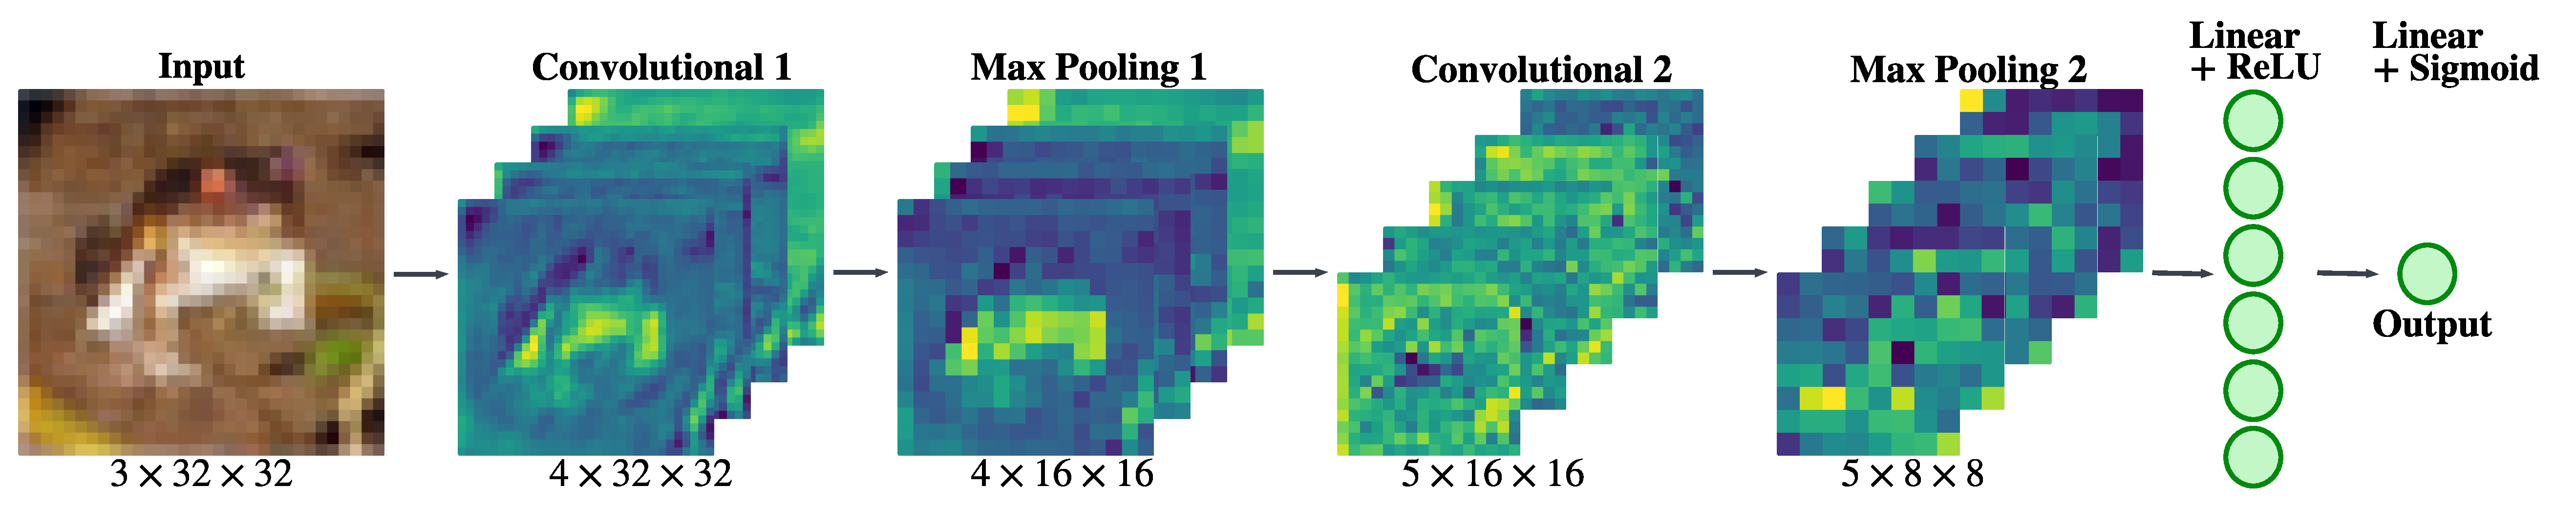
\includegraphics[width=1\textwidth]{./figures/neural_nets/CNN_frog.pdf}
    \caption{A binary classification CNN processing an image of a frog.}
    \label{fig:CNN_frog}
\end{figure}

Convolutional neural networks (CNNs) were initially designed to process image and, by extension, video data. Over time, they have been applied to processing far richer forms of data. A forward pass through a CNN designed for image processing is illustrated in \autoref{fig:CNN_frog}, in which we see that their architecture can be described on a high level as consisting of two parts. The first part performs feature extraction through convolution and pooling operations. The second part employs an MLP to produce the overall model's output given the earlier-extracted features, e.g. the probability that an input image is of a given class.

Before deep learning architectures became mainstream, researchers used handcrafted features (SIFT, HOG, SURF, etc.) for feature extraction and fed extracted features to a given model, e.g. an SVM for classification. That is, feature extraction wasn't learned, nor was it entwined with the inference component of their models. For image processing tasks, humans turn out to be far worse than deep learning architectures at knowing which features are most informative of what is being predicted. Hence, CNNs are now the go-to architecture for image and video processing. There's something to be said here about vision transformers and the extent to which they are competitive with CNNs but this can wait. Relevant interactive visualisation: \href{https://adamharley.com/nn_vis/cnn/3d.html}{\texttt{adamharley.com/nn\_vis/cnn/3d.html}}.

\subsubsection{Convolutions}
Convolution operations involve using a (typically square) matrix to, in some sense, summarise the information embedded in parts of the object over which it traverses. This matrix is referred to as a filter or a kernel — I prefer using filter as the term kernel has so many meanings elsewhere in maths. You can think of convolution operations as a sort of dot product between the given filter and the grid of pixel values over which lies during its traversal. For a simple illustration of this idea, consider \autoref{fig:convolution_operation}. Since CNNs consists of multiple convolution layers, the output of a convolution layer is often referred to as a feature map.

\begin{figure}[t]
    \centering
    \begin{minipage}{0.63\linewidth}
        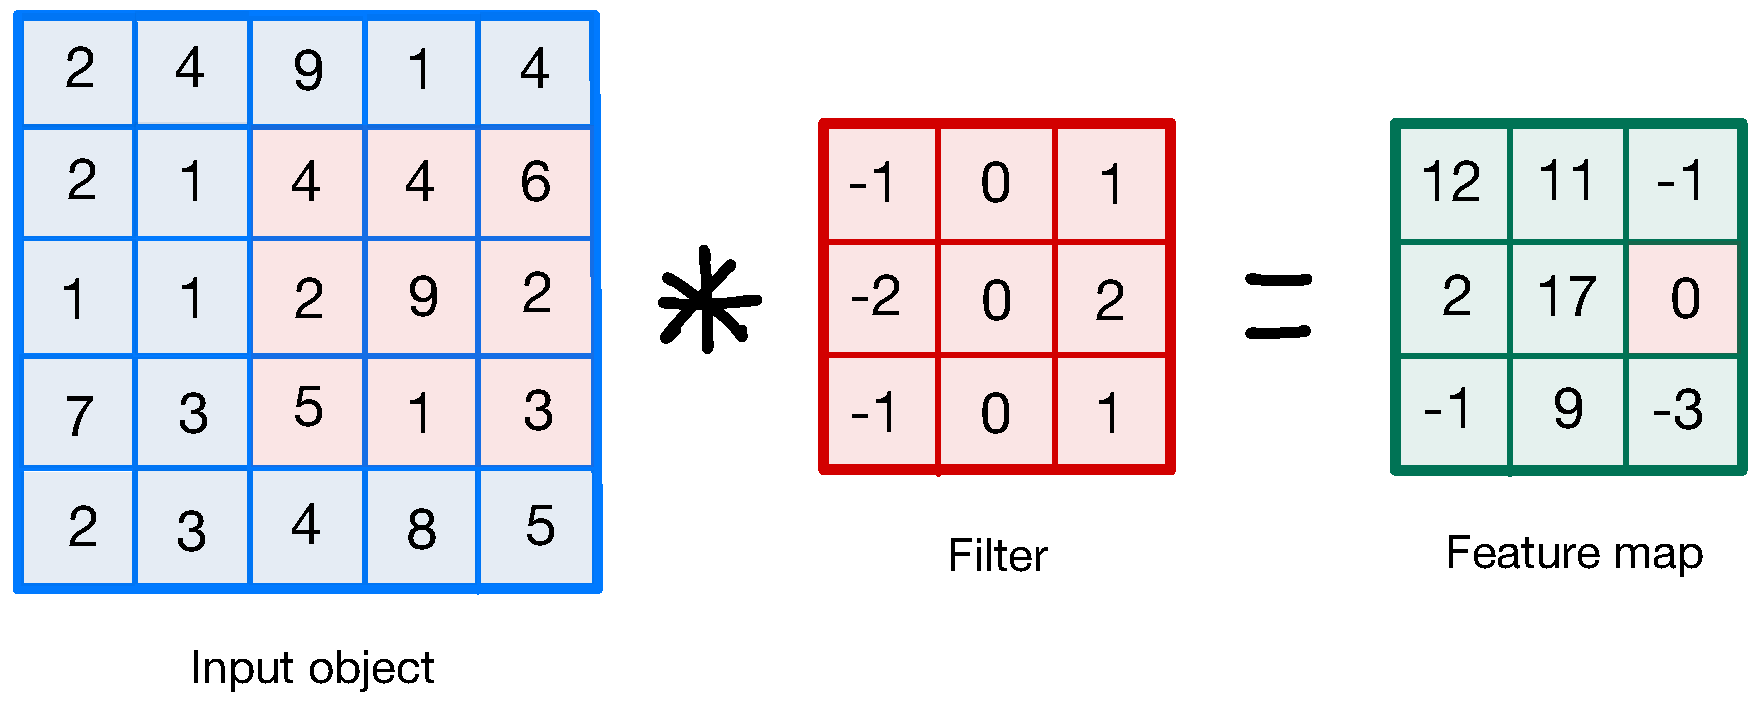
\includegraphics[width=\textwidth]{./figures/neural_nets/CNN_convolution.pdf}
    \end{minipage}%
    \hfill
    \begin{minipage}{0.35\linewidth}
        \caption{Convolution with a vertical edge detection filter with 0 bias.}
        \label{fig:convolution_operation}
    \end{minipage}
\end{figure}

More formally, given a feature map $I\in\mathbb{R}^{C\times W\times H}$ and a filter $K\in\mathbb{R}^{C\times k\times k}$ with $k<W$ and $k<H$, the feature map $F=K*I\in\mathbb{R}^{W'\times H'}$ is the convolution of $K$ over $I$ is as in
$$
F_{i,j}
=
\sum_{c=1}^C\sum_{x=1}^{k}\sum_{y=1}^{k}K_{c,x,y}\cdot I_{c,x+i,y+j}+b_c
$$
where $b_c$ is the filter's bias in channel $c$. Nowadays, $k=3$ is a very popular choice. Note that this notation is intended to illustrate what a convolution looks like algebraically. As it stands, what's written above does not account for padding, stride, etc.

Generally, earlier filters in a CNN architecture extract lower-level features, like edges and textures, while later convolutions extract higher-level features like entire components of object, e.g. wheels. This is illustrated in \autoref{fig:filter_levels}.

\begin{figure}[t]
    \centering
    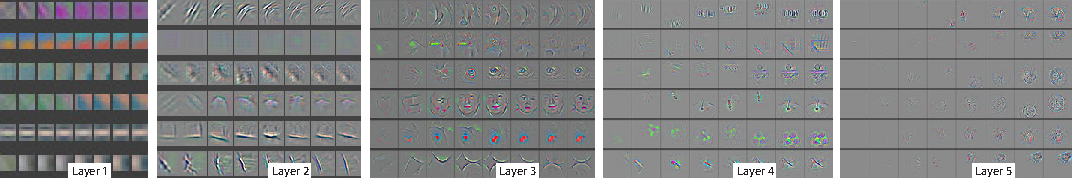
\includegraphics[width=\textwidth]{./figures/neural_nets/CNN_feature_levels.pdf}
    \caption{The level of abstraction of a CNN's learned filters. Earlier layers pertain to low-level features like edges or textures. Later layers pertain to higher-level features like faces or wheels.}
    \label{fig:filter_levels}
\end{figure}

\subsubsection*{Post-convolution spatial dimensions}
Given a feature map $F\in\mathbb{R}^{W\times H}$, suppose we compute the convolution $O\in\mathbb{R}^{W'\times H'}$ of the filter $K\in\mathbb{R}^{k\times k}$ over $F$ with uniform padding $P$ and stride $S$. The precise dimensions $W'$ and $H'$ of the new feature map $O$ are given by
$$
W'
=
\l\lfloor\frac{W+2P-k}{S}\right\rfloor+1
$$
and
$$
H'
=
\l\lfloor\frac{H+2P-k}{S}\right\rfloor+1.
$$
It's not too tricky to derive these. It's the kinda thing you do once and never again.

\subsubsection{Pooling}
Pooling operations reduce the spatial dimensions of a given feature map by applying relatively straightforward transformations: max pooling, min pooling, mean pooling, etc. There's not much point to expressing them rigorously. Instead, consider \autoref{fig:pooling}. Benefits of pooling are improved translation-invariance and reduced required compute.

\begin{figure}[ht]
    \centering
    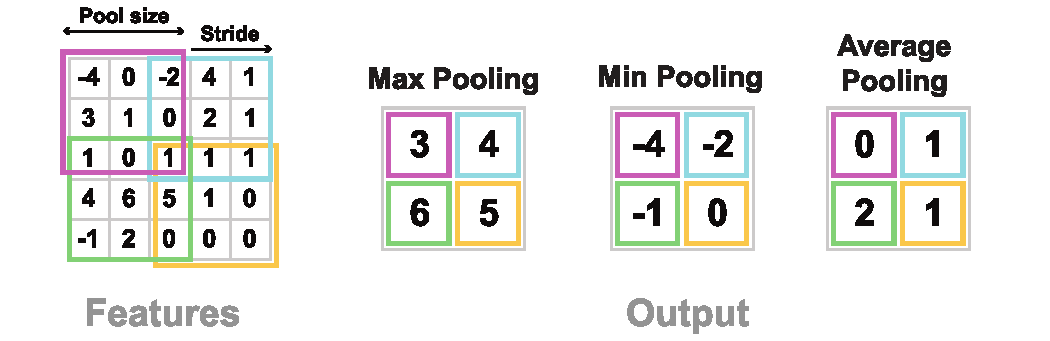
\includegraphics[width=\textwidth]{./figures/neural_nets/CNN_pooling.pdf}
    \caption{Common flavours of pooling.}
    \label{fig:pooling}
\end{figure}

\begin{tcolorbox}[title={\centering\textbf{Why use a CNN over an MLP?}}, colback=myLightBlue, colbacktitle=myDarkBlue, colframe=myDarkBlue, coltitle=white]
    Massively improved parameter-efficiency, translation invariance and learning efficiency\footnote{\href{https://ai.stackexchange.com/questions/27407/what-does-statistical-efficiency-mean-in-this-context}{\texttt{ai.stackexchange.com/questions/27407}}} (fewer samples needed to learn distributions to similar degrees of precision). These are in part due to the inductive bias present of their architecture.
\end{tcolorbox}

\subsubsection{Backpropagation for CNNs}

% recurrent neural networks
\subsection{\TODO Recurrent Neural Networks (RNNs)}

\subsubsection{Long Short-Term Memory (LSTMs)}
Schmidhuber

\subsubsection{Gated Recurrent Units (GRUs)}

% transformer models
\subsection{\TODO Transformers}
Just another (very effective) architecture for correlation extraction.

\subsubsection{Tokens and Embedding}
Tokenisation is the process of slicing a sample up into tokens. Think of splitting a $512\times512$ image into its four $256\times256$ quadrants or the sentence `The chef cooked a meal for the critic.' into
$$
\colorbox{purple}{The}\colorbox{green}{ chef}\colorbox{brown}{ cooked}\colorbox{red}{ a}\colorbox{teal}{ meal}\colorbox{blue}{ for}\colorbox{green}{ the}\colorbox{brown}{ critic}\colorbox{purple}{.}
$$
The purpose of tokenisation is self-explanatory: we'd like an idea of dependence between different parts of the input as to aid our output prediction.

An embedding function $E:\{1,\dots,|S|\}\to\mathbb{R}^d$, where $d\in\mathbb{N}$ is the embedding dimension, offers high dimensional numeric representations of tokens. What makes token embedding functions interesting is how well they can capture underlying semantics, e.g. of natural language. For example, an embedding function learned on pieces of text might satisfy
$$
E(\text{Germany})+E(\text{fascist})-E(\text{Mussolini})
\approx
E(\text{Hitler})
$$
for which the tokenisations occur.

\subsubsection{Positional encoding}
Use sinusoids to form a position vector $P_k$ for the $k$th token in an input sequence of length $L$. Add $P_k$ to the word embedding $E_k$ for $k=0,\dots,L-1$ to obtain the input $[E_0+P_0,\dots,E_{L-1}+P_{L-1}]$ fed to the model.

\subsubsection{Attention}
Has been around as an idea for a long time in less clear terms.

\subsubsection{Transformer blocks}
\dots

% misc. questions
\addtocontents{toc}{\protect\setcounter{tocdepth}{1}}
\subsection{Misc. questions}
\addtocontents{toc}{\protect\setcounter{tocdepth}{2}}

\begin{center}
    \textbf{\textcolor{blue}{Q1:} What is the purpose of activation functions?}
\end{center}
Without the application of at least one activation function, the values of the output neurons would simply be the result of matrix-vector multiplication and vector addition. That is to say, the output of the neural network, without an any activation function, would be a purely linear transformation of the input. The issue with this is that most problems require some degree of non-linearity. The staple example of this is the classification of two-dimensional samples which are not linearly separable. An example is illustrated in the left of \autoref{fig:non_linearly_separable}.

\begin{figure}[t]
    \centering
    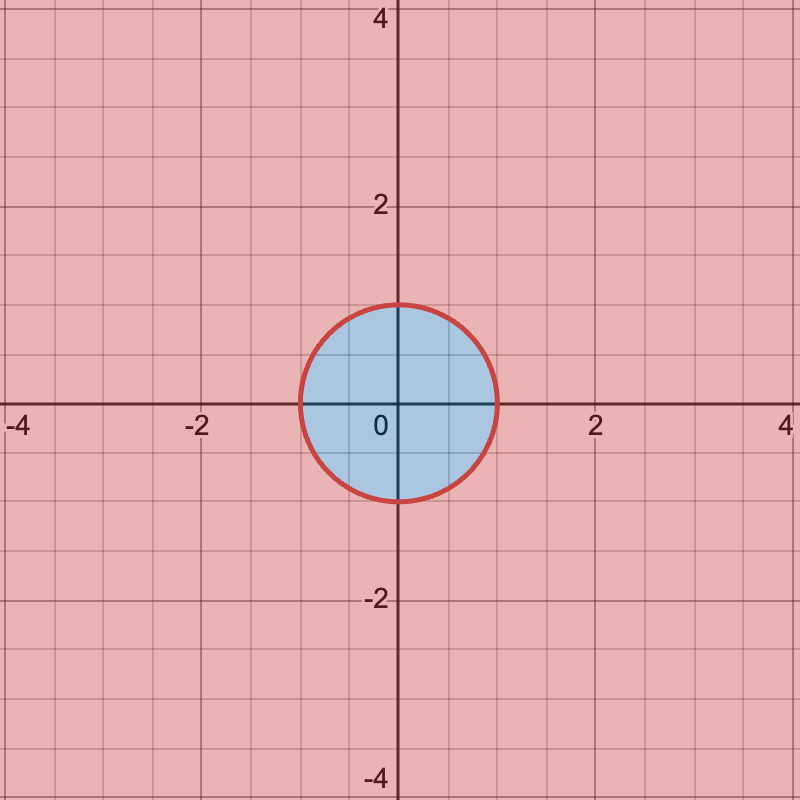
\includegraphics[width=0.40\columnwidth]{./figures/neural_nets/NLA_circle.png}
    \hspace{20pt}
    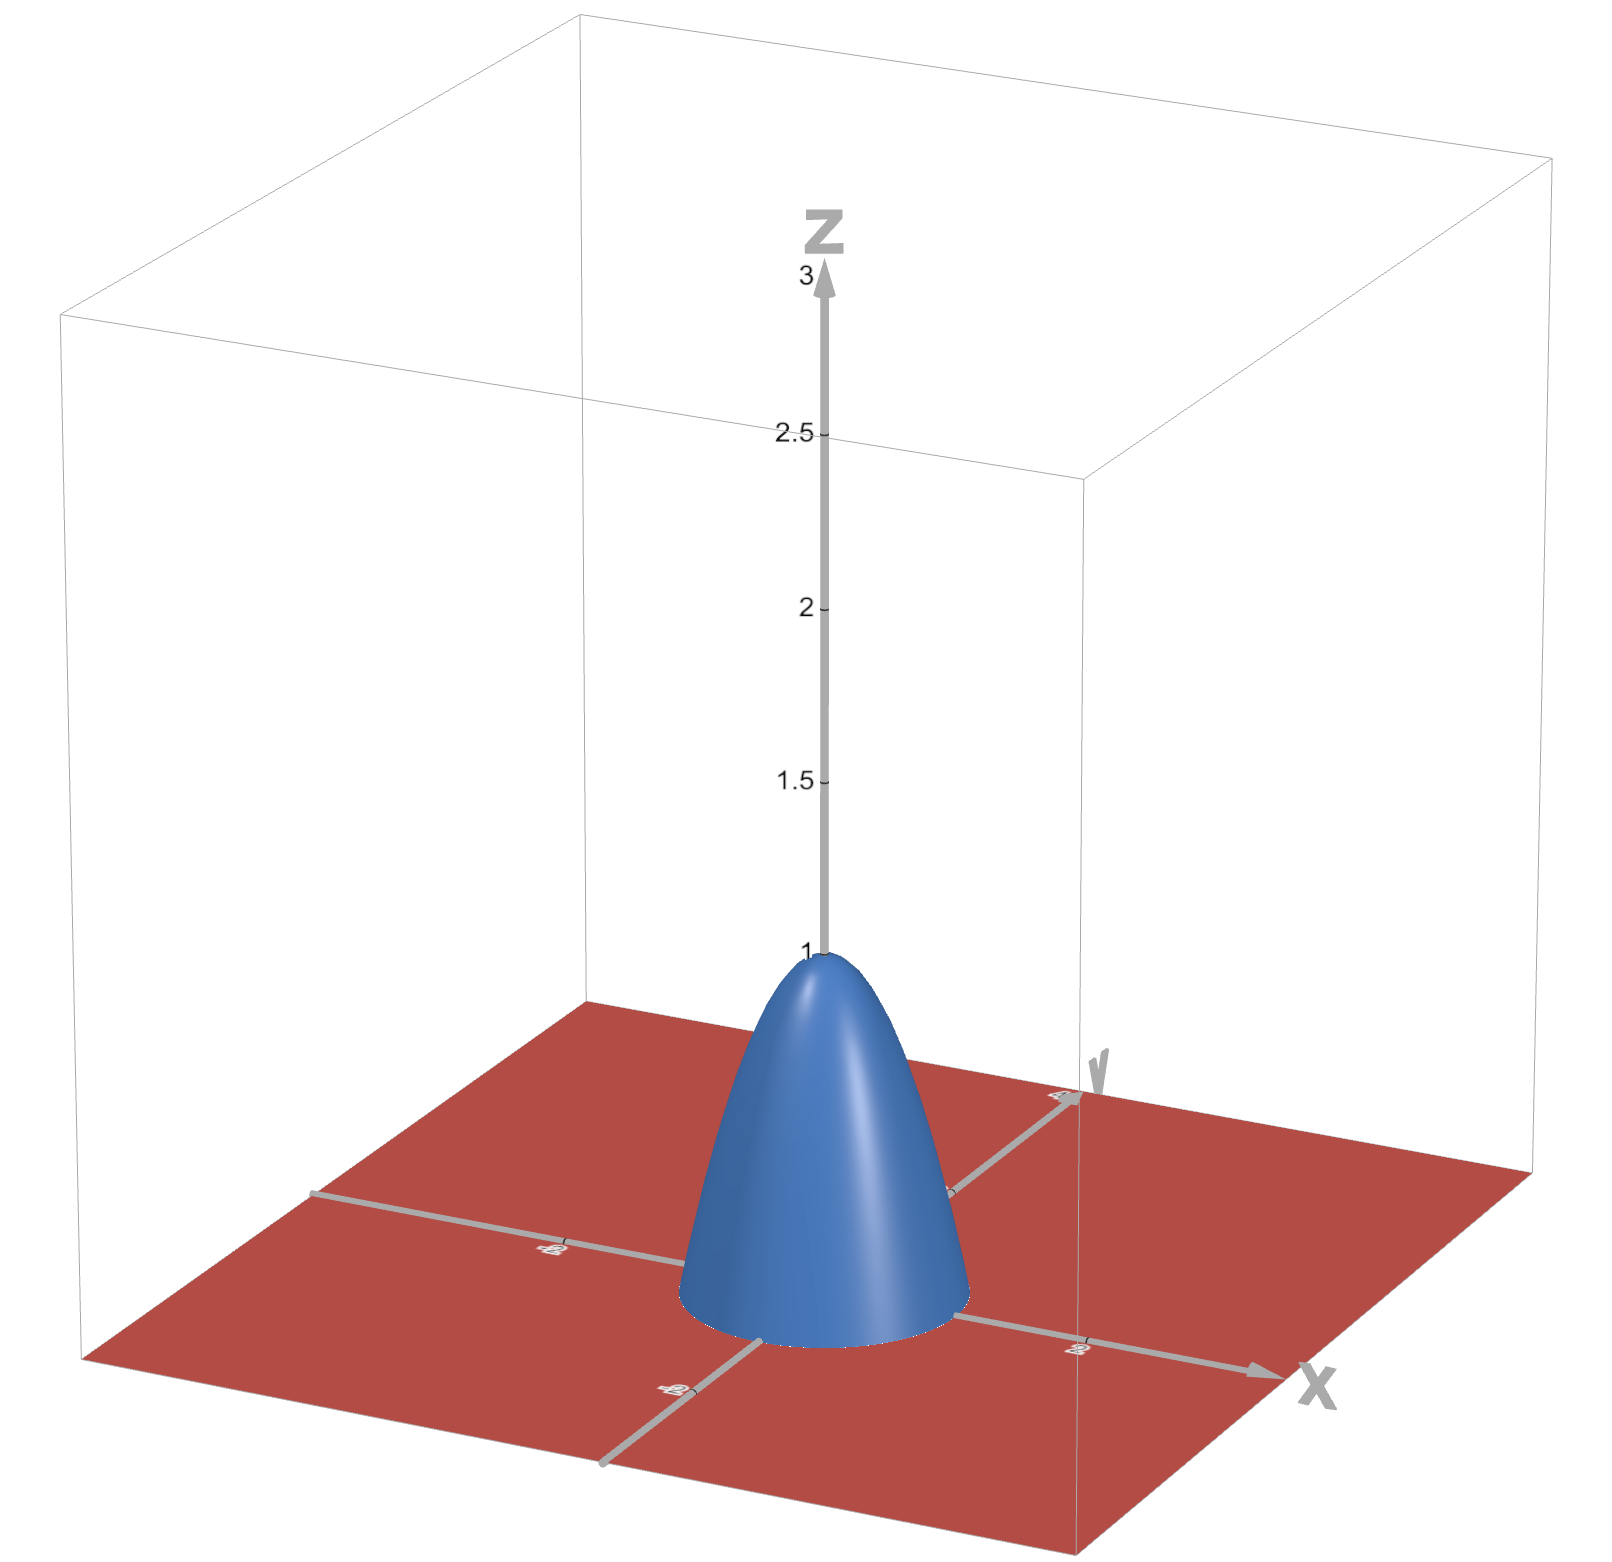
\includegraphics[width=0.40\columnwidth]{./figures/neural_nets//NLA_non_lin_transform.png}
    \caption{Non-linearly separable data (left) and its image under a non-linear transformation (right).}
    \label{fig:non_linearly_separable}
\end{figure}

The point is that there is no line that would separate the classes in either case: non-linearity is needed! In the latter case, it is desirable to be able to somehow punch the interior of the unit disc to form a blue mountain with the surrounding ground covered in red. This can be achieved by the non-linear transformation $\phi(x,y)=\max(0,1-(x^2+y^2))$ which is illustrated in the right of \autoref{fig:non_linearly_separable}.

From here, a natural linear decision boundary is the plane $z=0$ (i.e. the red ground surrounding the blue mountain). Any sample above the plane, i.e. any sample whose $z-$coordinate is positive, is classified as blue. It is otherwise classified as red. We can be more clever than this though. This transformation required us to map samples to 3D — how about mapping to just 1D? To do this, a complete decision function is given by
$$
D(x,y)=\l\lceil\frac{\l\lfloor x^2+y^2\right\rfloor}{x^2+y^2}\right\rceil
$$
and define $D(0,0)=0$ to account for the removable singularity.

\begin{center}
    \textbf{\textcolor{blue}{Q2:} Why not just one activation function in the output layer?}
\end{center}
If there were a single activation function towards the end of the architecture then everything that came before would be a series of linear transformations of the input. The composition of linear transformations is just a linear transformation. As such, said model would be equivalent to a single layer perceptron, i.e. linear transformation + non-linear activation function, which would yield linear decision boundaries only.

To be super pedantic, single-layer perceptrons yielding only linear decision boundaries is the case if the activation function used is monotonic, which is often the case. If you allow for weird, non-monotonic activations then this linear decision boundary result doesn't necessary hold but, again, this is a pretty pedantic detail.

\begin{center}
    \textbf{\textcolor{blue}{Q3:} Must activation functions be monotonic?}
\end{center}
Nope, it just makes things related to optimisation easier while having a sufficiently-small effect on performance in practice. Some results surrounding neural networks necessitate monotonic activation functions though.

\begin{center}
    \textbf{\textcolor{blue}{Q4:} Which activation functions should be used and when?}
\end{center}
Roughly speaking, I wouldn't worry too much about this in practice. The usual choices are all nice and differentiable (with small caveats, like with ReLU at 0) facilitating backpropagation. You should sometimes care about the output given the problem at hand. For example, if you need outputs in $[-1,1]$ then $\tanh$ is a natural choice.

Note that some choices, like Leaky ReLU, introduce hyperparameters to the model which can be undesirable, e.g. if one seeks to minimise the number of hyperparameters for the strength of their result (if there's no hyperparameter to cherry pick then your result is more trustworthy).

\begin{center}
    \textbf{\textcolor{blue}{Q5:} How does one prevent vanishing/exploding gradients?}
\end{center}
Skip connections help. Architectures which use them are sometimes called residual networks.
\begin{itemize}
    \item Most intuitive benefit: it helps prevent some layer in the architecture from degrading the input entirely. It's like a nice reminder to the model what it was working from before it got to this point
    \item Reduces vanishing or exploding gradients: opens the door to far deeper architectures
    \item Ensures that the model has to learn the residual as opposed to the full underlying function: faster convergence usually
    \item Takes pressure off parameter initialisation: if you set parameters to zero then initially model is just the identity and learning from there is feasible
\end{itemize}
It's worth mentioning that said vanishing behaviour can be observed during forward passes too.

% generative models (any other section name i've come up with has been due to overthinking)
\section{Generative Models}
Modelling data-generating processes is the heart of science: the laws which dictate graviation, \dots. The probabilistic equivalent of this idea is to model the joint probability function which, ideally, helps to answer probabilistic queries either exactly or approximately. While this section consists of methods of learning generative models pertaining to image-related distributions, the discussed methods are often applicable to generative modelling in general.

\begin{tcolorbox}[title={\centering\textbf{Terminology}}, colback=myLightBlue, colbacktitle=myDarkBlue, colframe=myDarkBlue, coltitle=white]
    To avoid having to write \textit{probability mass/density function} in full throughout this section, \textit{probability function} will be written.
\end{tcolorbox}

Put more precisely, what we further refer to as a generative probabilistic model is a tuple $(\X, p_{\Theta})$ consisting of model variables $\X=(X_1,\dots,X_m)$ and a probability function $p_{\Theta}:\Omega_{\X}\rightarrow\mathbb{R}_{\geq0}$ parameterised according to the parameter set $\Theta$. The probabilistic queries we might hope to answer given a generative probabilistic model include evidence queries $p(\x)$, marginal queries $p(\x')$, where is a realisation of some subset of the model variables, and sampling queries, in which one obtains a realisation of the model variables in conjunction.

The holy grail of generative probabilistic modelling is to find an exact, efficiently computed and algebraically manipulable representation of the underlying joint probability function of interest. If obtained, one can reason probabilistically with ease but, as we will see, the purpose, limitations and learning of generative probabilistic models varies heavily. To illustrate this, consider probabilistic graphical models (PGMs) which offer a graph structure in which conditional dependencies between model variables are expressed in a compact and human-interpretable manner. The most well-known class of PGMs are Bayesian networks.

% bayesian nets
\subsection{\IMPROVE Bayesian networks (BNs)}
A natural approach to representing the joint probability function of model variables is to decompose it into smaller probability functions and model those. For example, you might decompose the probability function according to the chain rule of probability as in
\begin{align*}
    p(x_1,\dots,x_m)
    &=
    p(x_1)p(x_2|x_1)\cdots p(x_m|x_1,\dots,x_{m-1})\\
    &=
    \prod_{i=1}^m p(x_i|x_1,\dots,x_{i-1}).
\end{align*}
From here, sampling may be done autoregressively: sample $x_1$ according to $p(x_1)$, $x_2$ according to $p(x_2|x_1)$ and so on until an entire realisation of $\X=(X_1,\dots,X_m)$ is obtained. Why stop at decomposition though? In an image, nearby pixel values may correlate but far away pixels may not, so why incoroporate them in the conditional? Why not learn the dependencies between the model variables? Boom, Bayesian networks.

\subsubsection{Formulating BNs}
With their motivation out of the way, we can move on to their formulation. A Bayesian network consists of a directed acyclic graph (DAG) $\mathcal{G}$ and a parameter set $\theta$. The graph $\mathcal{G}$ has a single node for each model variable $X_1,\dots,X_m$ and directed edges represent conditional dependencies. The parameter set $\theta$ pertains to the parameters of the conditional distributions induced by $\mathcal{G}$.

\begin{example}
    For model variables $X_1, X_2$ and $X_3$, if $X_3|X_1$ is independent of $X_2$ then their joint probability function may be decomposed as
    $$
    p(x_1,x_2,x_3)
    =
    p_{\theta_1}(x_1)p_{\theta_2}(x_2|x_1)p_{\theta_3}(x_3|x_1)
    $$
    whose corresponding DAG is given by
    \begin{center}
        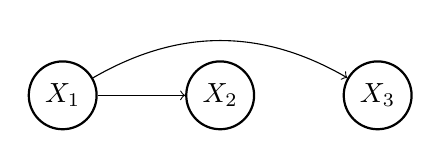
\begin{tikzpicture}[node distance=2cm, every node/.style={circle, draw, thick}]
            \node (A) {$X_1$};
            \node (B) [right of=A] {$X_2$};
            \node (C) [right of=B] {$X_3$};

            \draw[->] (A) -- (B);
            \draw[bend left][->] (A) edge (C);
        \end{tikzpicture}
    \end{center}
    Notice that the choice of $X_1$ as the model variable upon which nothing is conditioned is entirely arbitrary. As a result, for a given decomposition, DAGs are not unique. Here, $\theta=(\theta_1,\theta_2,\theta_3)$.
\end{example}

\subsubsection{Complexity of Inference}
Before considering how to learn a Bayesian network (its DAG and parameters), let's consider how Bayesian networks may be applied to inference. As far as exact inference goes, Bayesian networks have several pitfalls as far as probabilistic models go. Many probabilistic queries have complexity which is exponential in the tree-width of the Bayesian network. Known algorithms for these tasks are variable elimination and junction trees. To understand this crux, we must first understand tree-width.

As for approximate inference, perhaps the most well known algorithm is loopy belief propagation, developed by Judea Pearl, also known as sum-product message passing. Pearl writes a bunch of interesting things about it in his The Book of Why. It's worth noting that belief propagation is exact for tree-shaped Bayesian networks.

\subsubsection{Learning Structure}
Unlike the structure of neural network architectures, the structure of a Bayesian network (its DAG) can be motivated rigorously via maximum likelihood estimation. In brief, the likelihood of a given DAG can be computed and so a `best' DAG, according to MLE, can be computed. For Bayesian networks pertaining to Gaussian distributed variables, scoring can be done using Bayesian metric for Gaussian networks having score equivalence (BGe). For Bayesian networks pertaining to discretely distributed variables, scoring can be done using Bayesian Dirichlet likelihood equivalent (BDe).

\subsubsection{Learning Parameters}
\dots

% variational autoencoders
\subsection{\REVIEW Variational Autoencoders (VAEs)}
In describing variational autoencoders (VAEs), it's natural to first motivate autoencoders and then spice things up with variational inference do generative things.

% autoencoders
\subsubsection{Autoencoders: no variation yet!}
\label{sec:autoencoders}
An autoencoder $(\Omega_{\X},d,\phi,\theta)$ consists of a sample space $\Omega_{\X}\subset\mathbb{R}^m$, a latent dimension $d\in\mathbb{Z}_{\geq1}$, an encoder $\phi:\mathbb{R}^m\to\mathbb{R}^d$ and a decoder $\theta:\mathbb{R}^d\to\mathbb{R}^m$. Using a subset of $\Omega_{\X}$, one typically learns the encoder $\phi$ and the decoder $\theta$ with the goal of approximating the identity on $\Omega_{\X}$ via $\theta\circ \phi$. That is, roughly put, one seeks to obtain an encoder/decoder pair such that $\theta(\phi(\x))\approx\x$ for all $\x\in\Omega_{\X}$.

\begin{figure}[t]
    \centering
    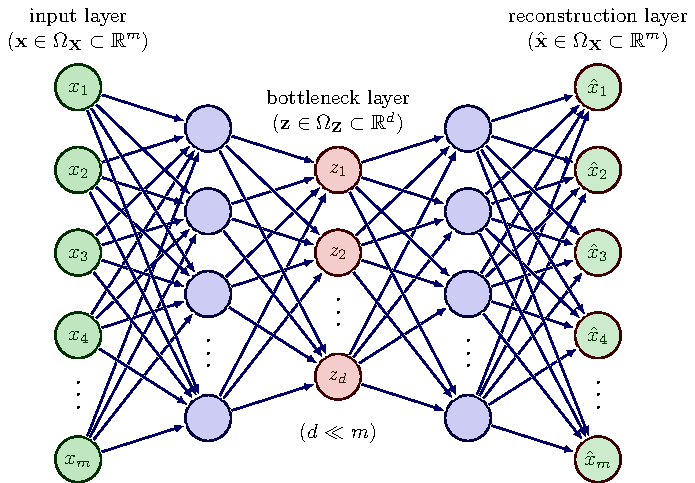
\includegraphics[width=\columnwidth]{./figures/generative_models/AE_autoencoder.pdf}
    \caption{An autoencoder in which $\phi$ and $\theta$ are fit using multi-layer perceptrons (MLPs).}
    \label{fig:autoencoder}
\end{figure}

In intuitive terms, one can see the encoder $\phi$ as a compressor of samples in $\Omega_{\X}$ to their compressed (or latent) representation in $\mathbb{R}^d$ and so one might refer to the image of $\phi$ as the latent space $\Omega_{\Z}$. Similarly, the decoder $\theta$ can be seen as a decompressor of compressed representations $\z\in\Omega_{\Z}$ yielding the original sample $\x$. In line with this notion of an autoencoder as a compressor/decompressor, the latent dimension $d$ is typically taken to be far smaller than the dimension of the distribution of interest, i.e. $d\ll m$. Of course, when $d\ll m$, learning such mappings $\phi$ and $\theta$ typically involves some loss of information if $\Omega_{\X}$ is a manifold whose intrinsic dimension is greater than $d$. That is, autoencoders are typically lossy compressors.

\begin{example}
    Suppose $\Omega_{\X}=\{(a,a,b)\in\mathbb{R}^3:||(a,a,b)||\leq1\}$ and $d=2$. One immediately notices that $\Omega_{\X}$ is a two-dimensional surface embedded in $\mathbb{R}^3$ as it is the intersection of the unit ball and the plane $\{(a,a,b):a,b\in\mathbb{R}\}$. To produce representations of $\x=(a,a,b)\in\Omega_{\X}$ in $\mathbb{R}^2$ (i.e. to compress a sample) one might employ the encoder $\phi_2(x,y,z)=(x,z)$. To reconstruct samples from their latent representation (i.e. to decompress) one might employ the decoder $\theta_2(x,z)=(x,x,z)$. The autoencoder $(\Omega_{\X},2,\phi_2,\theta_2)$ offers lossless compression on the sample space as $(\theta_2\circ\phi_2)(\x)=\x$ for all $\x\in\Omega_{\X}$.
    
    \hspace{15pt} If we instead desire latent representations of $\x=(a,a,b)\in\Omega_{\X}$ in $\mathbb{R}$, i.e. if $d=1$, one might employ the encoder $\phi_1(x,y,z)=x$ and the decoder $\theta_1(x)=(x,x,x)$. The autoencoder $(\Omega_{\X},1,\phi_1,\theta_1)$ offers lossy compression, i.e. some information pertaining to a sample is lost during its compression and decompression as $(\theta_1\circ\phi_1)(a,a,b)=(a,a,a)$ for all $a,b\in\mathbb{R}$.
\end{example}

One's tolerance for the loss incurred by a given encoder/decoder pair is task-dependent. Given a dataset $D=\{\x_1,\dots,\x_n\}\subset\Omega_{\X}$ and a latent dimension $d$, one might compute the pair $(\phi^*,\theta^*)\in\Phi\times\Theta$ which minimises the empirical risk over $D$ where $\Phi$ and $\Theta$ are chosen function families. That is, computing
$$
(\phi^*,\theta^*)
=
\argmin_{(\phi,\theta)\in\Phi\times\Theta}
\sum_{i=1}^n||\x_i-\theta(\phi(\x_i))||^2.
$$
If the function families permit the computation of gradients of $\phi\in\Phi$ and $\theta\in\Theta$ then this computation may be done using gradient descent. For example, one could take $\Phi$ and $\Theta$ to be the family of MLPs of appropriate input and output dimensions, as illustrated in \autoref{fig:autoencoder}.

\subsubsection{Motivating VAEs}
Autoencoders are great for compression, denoising, disecting LLMs (sparse autoencoders), etc. but we're yet to see how we might apply them to generative tasks, e.g. sampling from the complex underlying distribution $p(\x)$ from which their training dataset $\{\x_1,\dots,\x_n\}$ was sampled. An intuitive first idea is to train an autoencoder, randomly sample from its latent space and feed the sampled latent through the learned decoder, as in \autoref{fig:autoencoder_generation}. The outputs of the decoder should be similar to some subet of the training data, right? No.

\begin{figure}[t]
    \centering
    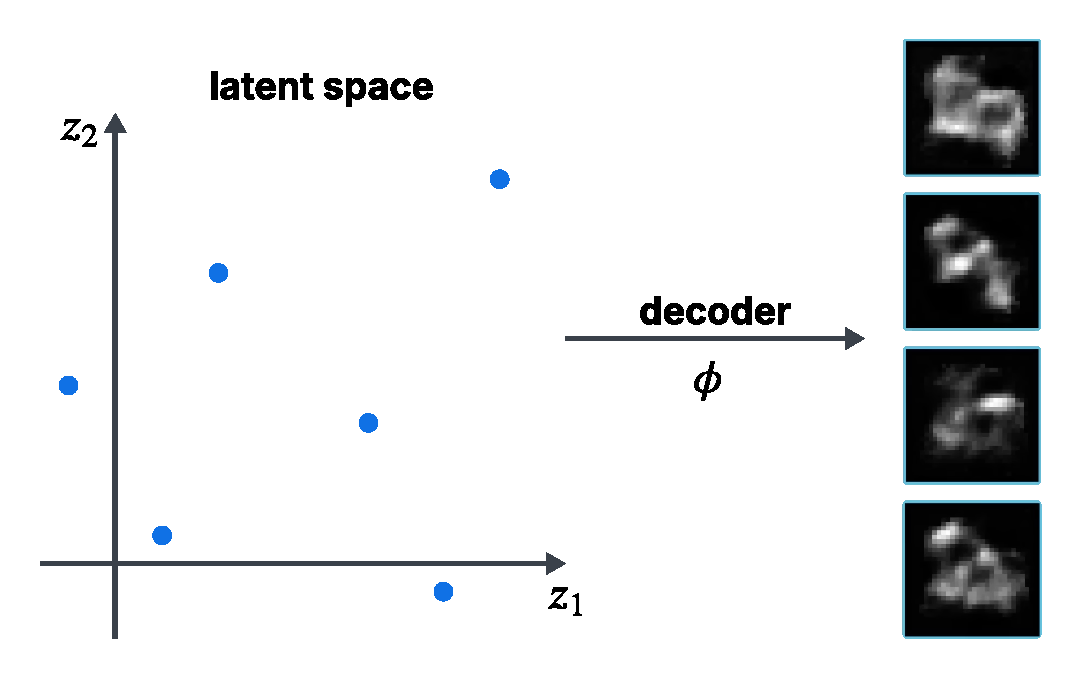
\includegraphics[width=0.49\columnwidth]{./figures/generative_models/AE_gen_1.pdf}
    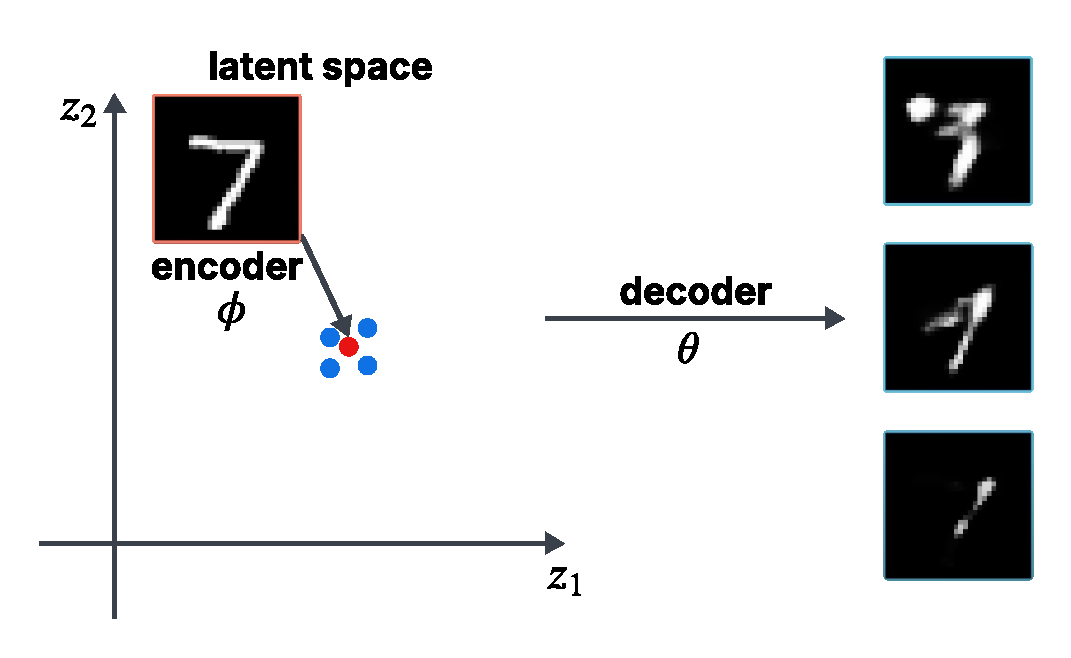
\includegraphics[width=0.49\columnwidth]{./figures/generative_models/AE_gen_2.pdf}
    \caption{Failed intuitive ideas for using an autoencoder as a generative model.}
    \label{fig:autoencoder_generation}
\end{figure}

Disaster strikes and we begin to see just how unstructured the latent space of an autoencoder is: randomly sampling from it and decoding yields nonsense outputs from the decoder because most of the latent space itself is meaningless (nothing is encoded to most of it, so in some sense a lot of it is `un-utilised'). This is perhaps unsurprising as at no point during training an autoencoder do we encourage it to interpolate nicely between encodings.

An intuitive second idea is to feed the decoder points in the latent space which are close to the encoding of a given training sample, as in \autoref{fig:autoencoder_generation}. The outputs of the decoder should be a sample of the class of said encoding's sample, right? No. Distaster strikes again. For meaningful decodings using this idea, one must take points in the latent space which are ridiculously close to this chosen sample's latent embedding. So close that you'd be practically reconstructing the original training sample each time — certainly not what we mean when we say that we'd like to generate new samples. So how do we do autoencoder-like things in a way that yields well-structured latent spaces? Variational autoencoders (VAEs) to the rescue!

\subsubsection{Formulating VAEs}
\begin{figure}[t]
    \centering % these widths are specific
    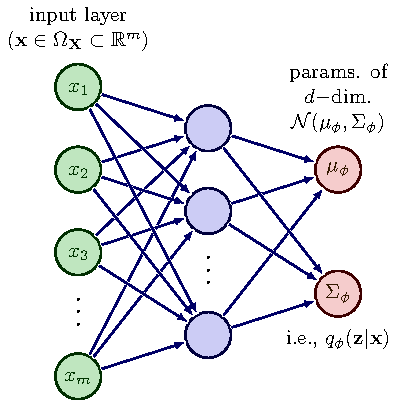
\includegraphics[width=0.46\textwidth]{figures/generative_models/VAE_encoder.pdf}
    \hfill
    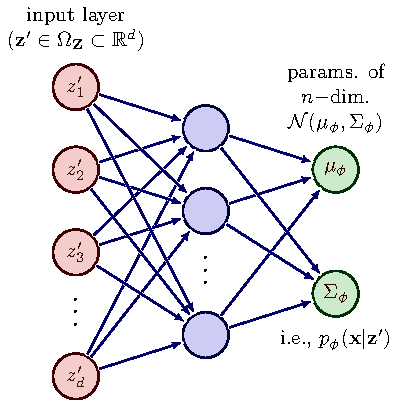
\includegraphics[width=0.46\textwidth]{figures/generative_models/VAE_decoder.pdf}
    \caption{Left: an encoder which outputs parameters of the latent distribution $q_{\phi}(\z|\x)=\mathcal{N}(\mu_{\phi},\Sigma_{\phi})$. Right: a decoder which outputs parameters of the reconstruction distribution $p_{\theta}(\x|\z')=\mathcal{N}(\mu_{\theta},\Sigma_{\theta})$ in which $\z'\sim q_{\phi}(\z|\x)$.}
    \label{fig:VAE_architecture}
\end{figure}

Leaving aside, for now, how to learn one from data, VAEs can informally be seen as an extension of autoencoders in which the encoder and decoder each output parameters of a distribution belonging to some pre-chosen distribution family. Extending the notation used to define autoencoders, a variational autoencoder $(\Omega_{\X},d,\mathcal{Q}_d,\mathcal{P}_m,\phi,\theta)$ consists of the sample space of the distribution of interest $\Omega_{\X}\subset\mathbb{R}^m$, a latent dimension $d\in\mathbb{Z}_{\geq1}$, the parameter space $\mathcal{Q}_d$ of a family of $d-$dimensional conditional distributions denoted $q_{\phi}(\z|\x)$, the parameter space $\mathcal{P}_m$ of a family of $m-$dimensional conditional distributions denoted $p_{\theta}(\x|\z)$, an encoder $\phi:\mathbb{R}^m\to\mathcal{Q}_d$ and a decoder $\theta:\mathbb{R}^d\to\mathcal{P}_m$.

To illustrate the intended meaning of the newly-introduced parameter spaces $\mathcal{Q}_d$ and $\mathcal{P}_m$, one's encoder might yield the expectation vector and covariance matrix of a $d-$dimensional Gaussian $\mathcal{N}(\mu,\Sigma)$, i.e. $\mathcal{Q}_d$ could be the parameter space of the family of $d-$dimensional Gaussian distributions yielding
$$
\mathcal{Q}_d
=
\{
(\mu,\Sigma):\mu\in\mathbb{R}^d, \Sigma\in\mathcal{S}_{++}^d
\}
=
\mathbb{R}^d\times\mathcal{S}_{++}^d
$$
where $\mathcal{S}_{++}^d$ denotes the set of all positive-definite matrices in $\mathbb{R}^{d\times d}$.

As the encoder of a VAE yields a $d-$dimensional distribution $q_{\phi}(\z|\x)$ given the sample $\x\in\Omega_{\X}$, to obtain a latent $d-$dimensional representation $\z'\in\mathbb{R}^d$ of $\x$, one computes the parameters $\phi(\x)\in\mathcal{Q}_d$ of $q_{\phi}(\z|\x)$, e.g. a $d-$dimensional Gaussian, via the encoder and samples $\z'\sim q_{\phi}(\z|\x)$. To reconstruct $\x$ from its latent representation $\z'$, one computes the parameters $\theta(\z')\in\mathcal{P}_m$ of the $q-$dimensional reconstruction distribution $p_{\theta}(\x|\z')$ via the decoder. Sampling $\x'\sim p_{\theta}(\x|\z')$ yields (ideally) a sufficiently-accurate reconstruction of the original sample $\x$. Achieving accurate reconstructions is done in a similar manner to autoencoders: by including a penalty term pertaining to reconstruction quality in the loss function used to learn the encoder and decoder.

Note that one's choice of $\mathcal{Q}_d$ and $\mathcal{P}_m$ should take into account the need to sample efficiently and so they should correspond to families of distributions which offer efficient means of sampling, e.g. Gaussians, as in \autoref{fig:VAE_architecture}.

\begin{example}
    Suppose $X_1\sim\mathcal{N}(1,2)$ and $X_3\sim\mathcal{N}(-1,1)$ are independent. Let $X_2=X_1+\epsilon$ where $\epsilon\sim\mathcal{N}(0,1)$ is independent of $X_1$ and $X_3$. If $X=(X_1,X_2,X_3)$ then $X\sim\mathcal{N}(\mu,\Sigma)$ with $\mu=(1,1,-1)'$ and the relevant covariance matrix $\Sigma$. As such, $\Omega_{\X}=\mathbb{R}^3$. To obtain two-dimensional representations of samples $\x\in\Omega_{\X}$ (so $d=2$), one might choose $\mathcal{Q}_2=\mathbb{R}^2\times\mathcal{S}_{++}^2$ and $\mathcal{P}_3=\mathbb{R}^3\times\mathcal{S}_{++}^3$. That is, we could fit a two-dimensional Gaussian to the latent space and a three-dimensional Gaussian to the reconstruction space. Knowing $X_2=X_1+\epsilon$, where $\epsilon\sim\mathcal{N}(0,1)$, one might choose the encoder
    \begin{align*}
        \phi&:
        \mathbb{R}^3\to\mathcal{Q}_2\\
        &(x_1,x_2,x_3)\mapsto((x_1,x_3),\sigma^2I_2)
    \end{align*}
    where $\sigma>0$ is small. That is, for a sample $(x_1,x_2,x_3)\in\Omega_{\X}$, the encoder's output would yield the latent distribution $q_{\phi}(\z|\x)=\mathcal{N}((x_1,x_3),\sigma^2I_2)$. As decoder, if all we desire is accurate reconstructions, we might choose
    \begin{align*}
        \theta&:
        \mathbb{R}^2\to\mathcal{P}_3\\
        &(z_1,z_2)\mapsto((z_1,z_1,z_2), \sigma^2I_3).
    \end{align*}
    That is, for the latent sample $\z'=(z_1',z_2')$, the decoder's output would yield the reconstruction distribution $p_{\theta}(\x|\z')=\mathcal{N}((z_1',z_1',z_2'),\sigma^2I_3)$. Ideally, sampling $(x_1',x_2',x_3')\sim p_{\theta}(\x|\z')$ would yield a sample sufficiently similar to the original sample $\x=(x_1,x_2,x_3)$.

    Note that in practice, one does not know the true distribution $p(\x)$ and so hand-picking the encoder and decoder as in this example is infeasible. Typically, the encoder and decoder are learned from a dataset $D\subset\Omega_{\X}$.
\end{example}

At this point, a natural question arises: for which tasks is learning a VAE more appropriate than learning an autoencoder? The answer lies in the purpose of VAEs which is two-fold: 1) to perform sufficiently-accurate compression/decompression and 2) to produce a sufficiently regularised approximation of the latent space $\Omega_{\Z}$. The latter is ensured by how one learns a VAE from data, which we soon consider. In brief, when learning an autoencoder one never imposes restrictions on the latent space beyond encouraging the model to yield sufficiently-accurate reconstructions. As a result, the latent space of an autoencoder is not well-structured. For example, for latent samples $\z_1,\z_2\in\Omega_{\Z}$ which are `close' in the latent space, their reconstructions are not necessarily `close' in $\mathbb{R}^m$. VAEs seek to remedy this.

To learn a VAE from data, we look to maximise the evidence lower bound (ELBO) over some dataset $D=\{\x_1,\dots,\x_n\}\subset\Omega_{\X}$. Over a single sample $\x\in\Omega_{\X}$, the ELBO is a tight lower bound of $\log(p(\x))$. As such, maximising the ELBO over $D$ can be seen as performing approximate maximum-likelihood estimation over $D$ (sometimes referred to as evidence maximisation). To derive the ELBO, first note that given a decoder $\theta$ (which parameterises the reconstruction distribution $p_{\theta}(\x|\z)$), we may express the marginal distribution $p(\x)$ using $p_{\theta}(\x|\z)$ as
\begin{equation}
\label{eq:marginal_likelihood}
p(\x)
=
\int p(\x,\z)d\z
=
\int p(\x|\z)p(\z)d\z
=
\int p_{\theta}(\x|\z)p(\z)d\z.
\end{equation}
Using \autoref{eq:marginal_likelihood}, along with the encoder $\phi$ (which parameterises the latent distribution $q_{\phi}(\z|\x)$) we derive the ELBO over a single sample $\x\in\Omega_{\X}$:
\begin{align*}
    \log(p(\x))
    &=
    \log\l(\int p_{\theta}(\x|\z)p(\z)d\z\r)\\
    &=
    \log\l(\int q_{\phi}(\z|\x)\frac{p_{\theta}(\x|\z)p(\z)}{q_{\phi}(\z|\x)}d\z\r)\\
    &=
    \log\l(\E_{\Z\sim q_{\phi}(\z|\x)}\l[\frac{p_{\theta}(\x|\Z)p(\Z)}{q_{\phi}(\Z|\x)}\r]\r)\\
    &\geq
    \E_{\Z\sim q_{\phi}(\z|\x)}\l[\log\l(\frac{p_{\theta}(\x|\Z)p(\Z)}{q_{\phi}(\Z|\x)}\r)\r]\\
    &=
    \E_{\Z\sim q_{\phi}(\z|\x)}\l[\log(p_{\theta}(\x|\Z))\r]-\E_{\Z\sim q_{\phi}(\z|\x)}\l[\log\l(\frac{q_{\phi}(\Z|\x)}{p(\Z)}\r)\r]\\
    &=
    \E_{\Z\sim q_{\phi}(\z|\x)}\l[\log(p_{\theta}(\x|\Z))\r]-D_{\text{KL}}(q_{\phi}(\Z|\x)||p(\Z))\\
    &=:
    \text{ELBO}
\end{align*}
in which the inequality arises due to Jensen's inequality, as in $\E[\log(f(\Z))]\leq\log(\E[f(\Z)])$, and $D_\text{KL}(Q||P)$ denotes the KL-divergence between distributions $Q$ and $P$, which is detailed in the appendix. The effect of maximising
$$
\text{ELBO}
=
\E_{\Z\sim q_{\phi}(\z|\x)}\l[\log(p_{\theta}(\x|\Z))\r]-D_{\text{KL}}(q_{\phi}(\Z|\x)||p(\Z))
$$
over a dataset is often explained term-by-term. The first term is a principled measure of the VAE's ability to reconstruct latent representations, as with autoencoders. The second term is a principled measure of the similarity of the latent distribution $q_{\phi}(\z|\x)$ and the prior $p(\z)$. The prior is chosen before training and the most common choice is a $d-$dimensional standard Gaussian, i.e. $p(\z)=\mathcal{N}(0,I_d)$. As such, minimising the negative KL-divergence between the latent distribution and said prior is often interpreted as encouraging the learning of the encoder such that latent representations are distributed according to the prior. This is particularly useful in the case that one is learning a VAE to generate new samples from $\Omega_{\X}$: post-training, sample $\z'\sim p(\z)$, compute the parameters $\theta(\z')$ of the reconstruction distribution $p_{\theta}(\x|\z')$ via the decoder and sample from it. Note that using a VAE for generative purposes does not invoke the use of the encoder, only the decoder is required post-training.

Given a dataset $D=\{\x_1,\dots,\x_n\}\subset\Omega_{\X}$, we learn a VAE by choosing function classes $\Phi$ and $\Theta$ (e.g. MLPs as in \autoref{fig:VAE_architecture}) and computing
$$
\argmax_{(\phi,\theta)\in\Phi\times\Theta}
\l[
\sum_{i=1}^n
\E_{\Z\sim q_{\phi}(\z|\x_i)}\l[\log(p_{\theta}(\x_i|\Z))\r]-D_{\text{KL}}(q_{\phi}(\Z|\x_i)||p(\Z))
\r].
$$
In practice, after choosing a latent dimension $d$, we often take $p(\z)=\mathcal{N}(0,I_d)$, $\mathcal{Q}_d=\mathbb{R}^d\times\mathcal{S}_{++}^d$ and $\mathcal{P}_m=\mathbb{R}^m\times\mathcal{S}_{++}^m$, i.e. Gaussians for the latent and reconstruction distribution families and the standard $d-$dimensional Gaussian for the prior. A benefit of these choices is that it yields a differentiable and easy-to-implement closed form for the KL-divergence term in the ELBO. Additionally, the expectation pertaining to the reconstruction term is typically approximated via a single sample, boiling down to a mean square error term\footnote{\url{https://n8python.github.io/mnistLatentSpace/}}.

\subsubsection{Backpropagation for VAEs}
To find suitable parameters of a given VAE architecture using gradient descent, we require that the ELBO is differentiable. With respect to $\theta$, the gradient is approximated according to
\begin{align*}
    \nabla_{\theta}\text{ELBO}
    &=
    \E_{\Z\sim q_{\phi}(\z|\x)}\l[\log(p_{\theta}(\x|\Z))\r]\\
    &=
    \frac{1}{k}\sum_{j=1}^k \nabla_{\theta}\log(p_{\theta}(\x|\z_j))
\end{align*}
which is no issue when the decoder's architecture is backpro-compatible. However, with respect to $\phi$, the gradient of the ELBO is less friendly.

% In practice, the expectation term in the ELBO is often approximated as in
% $$
% \E_{\Z\sim q_{\phi}(\z|\x_i)}\l[\log(p_{\theta}(\x_i|\Z))\r]
% \approx
% \frac{1}{k}\sum_{j=1}^k\log\l(p_{\theta}(\x_i|\z_j)\r)
% $$
% which requires sampling $\z_1,\dots,\z_k$ according to $q_{\phi}(\z|\x)$. Sampling, as a function, is not differentiable: reparameterisation trick to the rescue! Instead, independently sample $\epsilon_1,\dots,\epsilon_k$ according to $\mathcal{N}(0, I)$ and approximate the expectation by
% $$
% \frac{1}{k}\sum_{j=1}^k\log\l(p_{\theta}(\x_i|\mu_{\phi}(\x_i)+\sigma_{\phi}(\x_i)\odot\epsilon_j)\r)
% $$
% where $\odot$ denotes element-wise multiplication.

\subsubsection{Quirks of VAEs}
Blur outside of central object.

% general adversarial networks
\subsection{\IMPROVE Generative Adversarial Networks (GANs)}
To motivate generative adversarial networks (GANs), first consider what we want a generative model to do: produce convincing samples. As such, if there is some method of distinguishing real samples from those produced by a generative model, a perfect model would be able to fool the method. That is, the decisions made by the discriminative model should be akin to random guessing if the generative model is particularly good. This idea was realised by Ian Goodfellow while at a bar (the story is detailed in Genius Makers). From what I recall, there are disputes over whether or not the idea should be attributed to someone else. I'll look into it at some point.

This is precisely the idea that motivates GANs with inspiration taken from game theory. A GAN consists of a generative component $G:\Omega_{\Z}\to\Omega_{\X}$ and a discriminative component $D:\Omega_{\X}\to\{0,1\}$, which are trained in parallel. That is, $G$ produces a new sample given a latent $\z\in\Omega_{\Z}$ while $D$ learns to distinguish between training samples and outputs of $G$. Essentially, the models compete. In terms of loss functions, the discriminator employs binary cross entropy, as in
$$
\mathcal{L}_D
=
-\E_{\X}\l[\log(D(\X))\r]-\E_{\Z}\l[\log\l(1-D(G(\Z))\r)\r]
$$
and the generator makes use of
$$
\mathcal{L}_G
=
-\E_{\Z}\l[\log(D(G(\Z)))\r].
$$
As for architectures, the usual choices are natural: the disrciminator is fit using a CNN and the generator is fit using a deconvolutional CNN. So, as with other image generative models, to generate a new sample, we sample Gaussian noise and run it through the deconvolution process.

\begin{figure}[t]
    \centering
    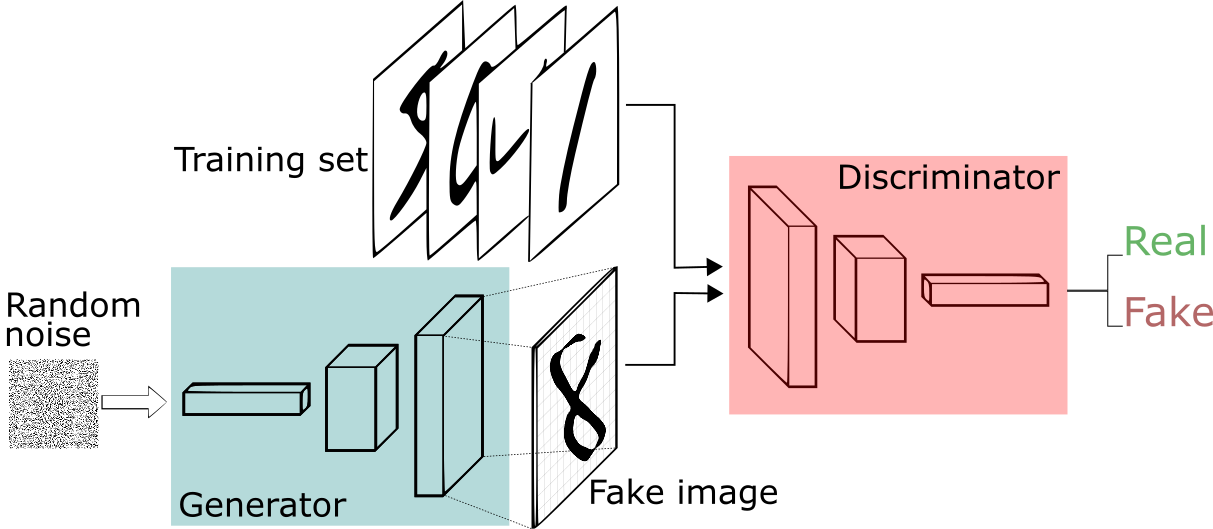
\includegraphics[width=\textwidth]{./figures/generative_models/GAN_architecture.png}
    \caption{Example GAN architecture.}
    \label{fig:GAN_architecture}
\end{figure}

\subsubsection{Quirks of GANs}

\begin{itemize}
    \item[--] Training them is a fucking headache. Constant model collapse.
    \item[--] GANs for non-image generation are hard to train.
    \item[--] Bluriness
\end{itemize}

\subsubsection{Flavours of GANs}
Perhaps the most important contribution of GAN-related things is not the vanilla generative model itself but the many flavours in which it comes: conditional GANs, cycle GANs, multiple player GANs, style GANs, etc.

% normalising flow models
\subsection{\TODO Normalising Flows}
Learn a bunch of bijections between distributions starting with the complex distribution from which we would like to sample and an isotropic Gaussian. Sample from the isotropic Gaussian and run it through the composition of said bijections to obtain a sample from the distribution of interest.

% diffusion models
\subsection{Diffusion Models}
The purpose of diffusion models is to facilitate the generation of samples from complex distributions from which sampling is typically intractable. While this overarching motive is not unique to diffusion models, how a diffusion model learns and how it generates new samples is quite distinct from other well-known generative models like VAEs and GANs (though some ideas are certainly comparable). A diffusion model can be described by its forward (noising) and backward (denoising) processes. Its forward process iteratively noises a sample $\x_0\in\mathcal{X}$, belonging to the distribution of interest, $T$-many times to obtain its noised equivalent $\x_T$. Formally, this is done via the Markov process
$$
q(\x_t|\x_{t-1})
=
\mathcal{N}\l(\x_t\Big|\sqrt{1-\beta_t}\x_{t-1},\beta_tI\r)
$$
where $\beta_1,\dots,\beta_T\in[0,1]$ are hyperparameters satisfying $\beta_i<\beta_{i+1}$, often referred to as the noise schedule of the model. With an appropriately chosen final time $T$, these noised equivalents $\x_T$ are akin to random noise sampled from $\mathcal{N}(0,I)$.

\begin{figure}[t]
    \centering
    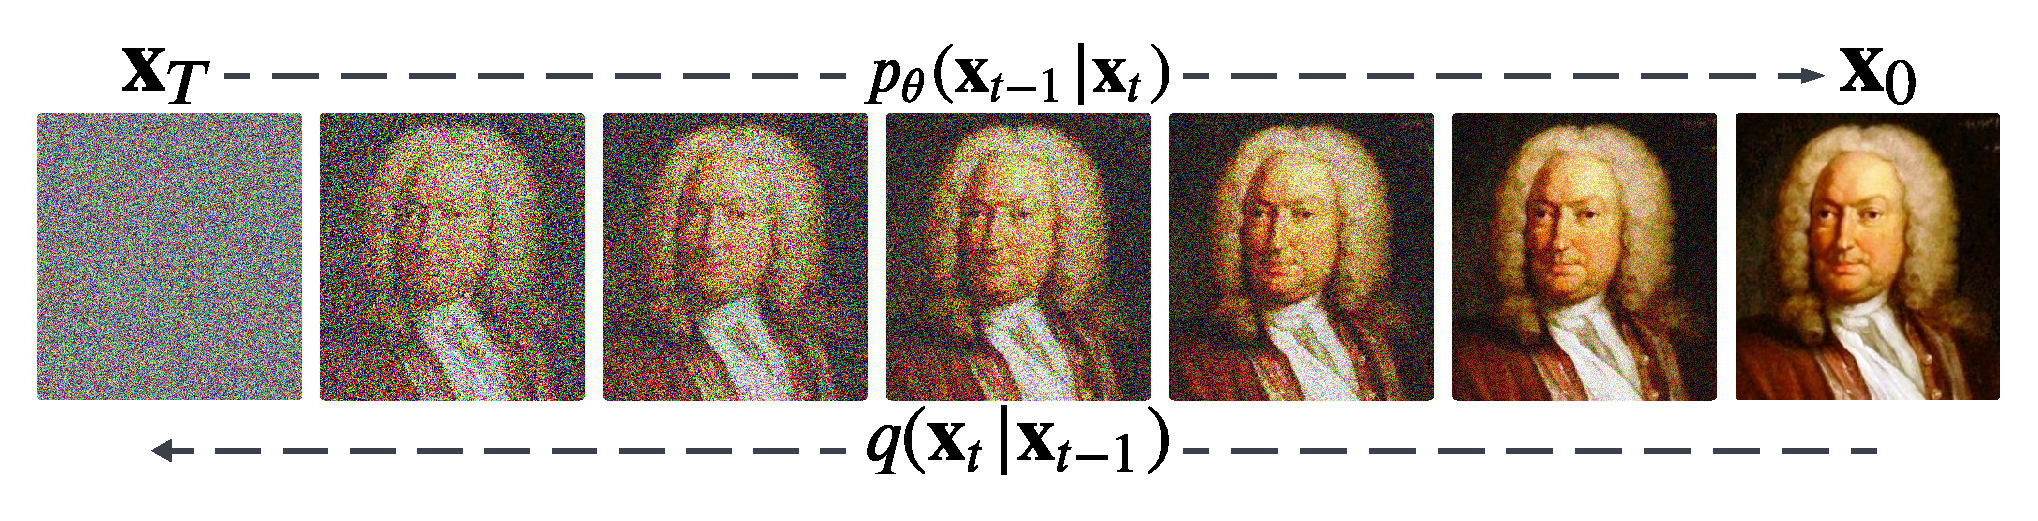
\includegraphics[width=\textwidth]{./figures/generative_models/diffusion_process.pdf}
    \caption{Johann Bernoulli being denoised in line with the backward process of a diffusion model.}
    \label{fig:diffusion_process}
\end{figure}

Letting $\alpha_t=1-\beta_t$ and $\Bar{\alpha}_t=\prod_{i=1}^t\alpha_i$, we can describe the backward process of a diffusion model again as a Markov process in which we sample some random noise $\x_T$ from $\mathcal{N}(0,I)$ and obtain the $(t-1){\text{st}}$ denoised sample from $p_{\theta}(\x_{t-1}|\x_t)$ via
$$
\x_{t-1}=\frac{1}{\sqrt{\alpha_t}}\l(\x_t-\frac{1-\alpha_t}{\sqrt
{1-\bar{\alpha}_t}}\epsilon_{\theta}(\x_t,t)\r)+\sigma_t\z
$$
where $\sigma_1,\dots,\sigma_T$ are hyperparameters, $\epsilon_{\theta}$ is the diffusion model's denoiser and $\z$ is sampled from $\mathcal{N}(0,I)$. % For clarity, $p_{\theta}(\x_{t-1}|\x_t)=\mathcal{N}(\x_{t-1}|\mu_{\theta}(\x_t,t),\sigma_tI)$ where $\mu_{\theta}(\x_t,t)$ is determined by the decoder $\epsilon_{\theta}$, the current noised image $\x_t$ and the time step $t$.
The purpose of the denoiser $\epsilon_{\theta}$, where $\theta$ is its tuple of parameters, is akin to its name: it is used to iteratively turn sampled noise $\x_T\in\mathcal{N}(0,I)$ into something resembling a sample $\x_0\in\mathcal{X}$ from the distribution of interest. If the architecture of its denoiser can be backpropagated through then training a diffusion model can be done in the usual manner of choosing an appropriate loss function and performing gradient descent in which gradients are computed via backpropagation through the entire model. We leave further details of training a diffusion model out for the sake of brevity but these can easily be found in literature.

So, what is an appropriate choice for the architecture of a diffusion model's denoiser? Before considering transformers for this task, we consider a more often-used choice, U-Net: a class of convolutional neural networks (CNNs).

\subsubsection{U-Net denoisers}
Despite not being the choice of denoiser made in the seminal paper introducing diffusion models, U-Net became the go to choice of denoiser architecture for contemporary diffusion models. To understand U-Net's popularity in this regard, it is worth understanding its architecture which consists of a contracting branch, terminating at its bottleneck, followed by an expansion branch, illustrated in \autoref{fig:u_net_arch}. This architecture can be thought of as forming a `U'-like shape, with the bottleneck lying at the bottom, hence its name.

\begin{figure}[t]
    \centering
    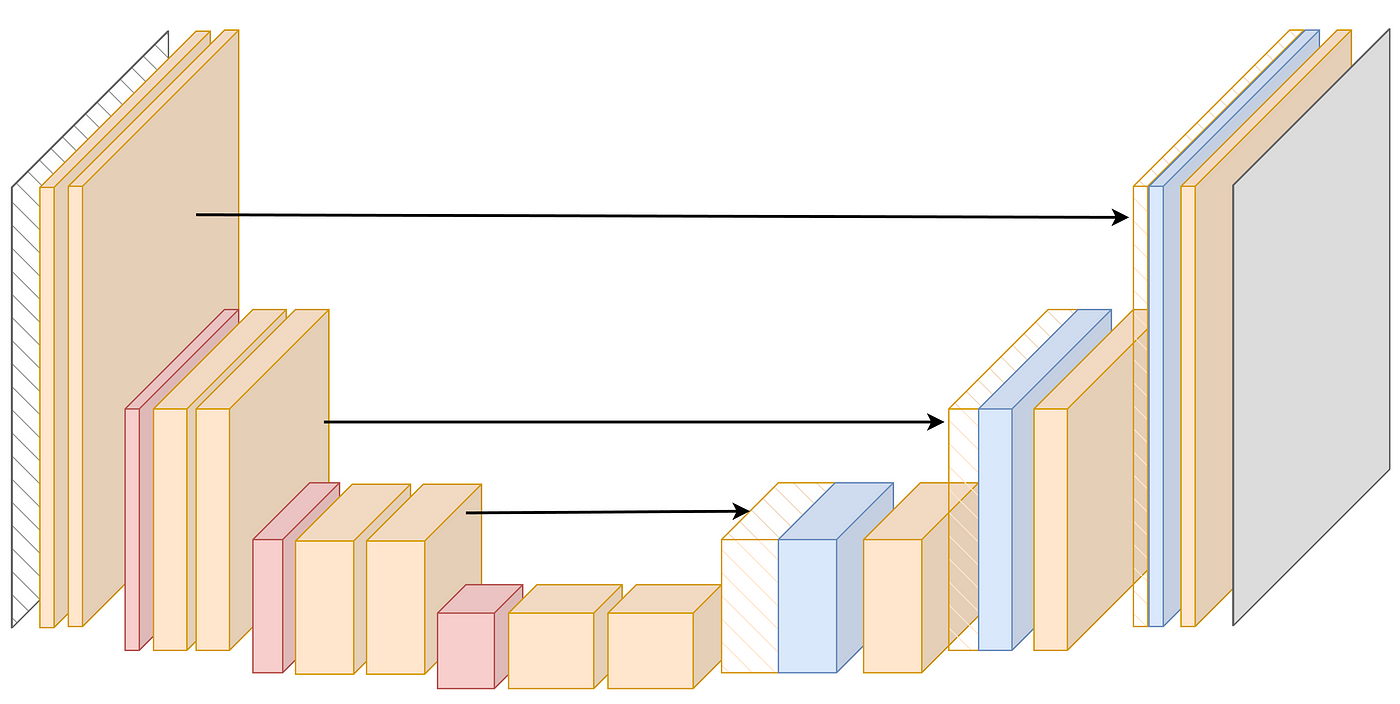
\includegraphics[width=\textwidth]{./figures/generative_models/unet.png}
    \caption{Example U-Net architecture.}
    \label{fig:u_net_arch}
\end{figure}

In the context of denoising, the contraction branch takes a noised image as input and iteratively completes a series of convolution operations followed by max pooling until reaching the bottleneck layer. At the bottleneck, the model has heavily reduced the spatial dimension of the input image while extracting varying levels of feature abstractions. For example, after the first iteration of convolution and max pooling, the spatial dimension of the input image may be reduced from $1024\times1024$ to $512\times512$ but edges and textures within the original image may be encoded in the feature maps at this stage. Then, during expansion, the model looks to upscale from the bottleneck in a way that retains the underlying image while removing noise. This is done by iteratively completing a series of deconvolutions, which correspond to upscaling, and using skip connections from its corresponding component in the contraction branch, seen in \autoref{fig:u_net_arch}, in order to retain the underlying image. With this in mind, it is clear why U-Net has been the go to choice of denoiser when developing a diffusion model.

% model evaluation
\subsection{\TODO Evaluating Generative Models}
Since samples are not labeled, how does one evaluate a generative model? What does under/overfitting mean for generative models?

% % object detection
% \section{Object Detection Models}

% Object detection is the task of localisation and classification within an image or video. Before the era of deep learning, it was typically solved using Haar-like filters\dots As of August 2025, there are three flavours of object detection models: R-CNN, YOLO and DETR.

% % R-CNN
% \subsection{\TODO (Fast/Faster) R-CNN}
% R-CNN models has evolved significantly since its proposal in 2013 with three evolutions worthy of a new name: R-CNN (the original), Fast R-CNN and Faster R-CNN. R-CNN stands for \textit{Regions with CNN features}. Roughly put, R-CNN model consist of two steps:
% \begin{enumerate}
%     \item Proposing regions of interest within the image
%     \item Classifying what is in each region (if there is something in the region)
% \end{enumerate}

% % YOLO
% \subsection{\TODO YOLO}

% % DETR
% \subsection{\TODO DETR}

% % future sections
% \section{To-be-included sections, one day}
% I'll get around to including these sections one day.

% % unsupervised learning
% \subsection{Unsupervised Learning}
% ain't no labels available to do supervised learning

% \subsubsection{Principal Component Analysis}
% bunch of linear algebra

% \subsubsection{$k$-means Clustering}
% what i think of when i think of clustering, easy example of latent variable

% \subsubsection{Autoencoders}
% already written in the variational autoencoder subsection

% % self-supervised learning
% \subsection{Self-supervised Learning}
% some labelled some ain't

% % nlp
% \subsection{Natural Language Processing (NLP)}
% blelele distributional semantics
% \begin{quote}
%     ``You shall know a word by the company it keeps." - some linguist
% \end{quote}

% appendices
\newpage
\begin{appendices}
\addtocontents{toc}{\protect\setcounter{tocdepth}{0}}

% probability things
\section{Probability Theory Things}
Here are some probability theory things, e.g. brief statements, long derivations, and so on, which belong in an appendix. I wish my understanding of probability theory, measure theory, stochastic processes, etc. were better. In another life.

For visual reminders, consider \href{https://seeing-theory.brown.edu/index.html}{\texttt{seeing-theory.brown.edu/index.html}}.

\subsection{Derivations Related to Common Distributions}
Probabilities pertaining to parameters, as in Bernoulli or categorical distributinos, are denoted by $p$ in this subsection. Hopefully this isn't too confusing due to $p$ being used to denote probability functions elsewhere in the document.

\subsubsection{From Bernoulli to Binomial}
Let's try to extend the Bernoulli distribution to the binomial distribution. If $X\sim\text{Ber}(p)$ then $\Omega_X=\{0,1\}$ and $\mathbb{P}(X=x)=p^x(1-p)^{1-x}$.

Taking $n$ independent Bernoulli random variables and summing them yields the random variable $\X=\sum_{i=1}^nX_i\sim\text{Bin}(n,p)$ with $\Omega_{\X}=\{0,\dots,n\}$. Let $k$ denote a realisation of $\X$, i.e. $k=x_1+\dots+x_n$. The corresponding mass function is given by
\begin{align*}
    \mathbb{P}(\X=k)
    &=
    Z\cdot\prod_{i=1}^n\mathbb{P}(X_i=x_i)\\
    &=
    Z\cdot\prod_{i=1}^np^{x_i}(1-p)^{1-x_i}\\
    &=
    Z\cdot p^{x_1+\dots+x_n}(1-p)^{n-(x_1+\dots+x_n)}\\
    &=
    Z\cdot p^k(1-p)^{n-k}
\end{align*}
where $Z$ is a normalising constant such that $\sum_{k=0}^nZp^k(1-p)^{n-k}=1$. It's more intuitively seen as the number of ways of placing $k$-many $1$s among a series of $n\geq k$ bits, i.e. $Z=\binom{n}{k}$, so
$$
\mathbb{P}(\X=k)
=
\binom{n}{k}p^k(1-p)^{n-k}.
$$

\subsubsection{From Categorical to Multinomial}
The categorical distribution is an extension of the Bernoulli distribution and the multinomial distribution is an extension of the binomial distribution. In line with this, we'd hope to be able to extend the categorical distribution to the multinomial distribution.

If $X\sim\text{Cat}(p_1,\dots,p_C)$ then realisations of $X$ can be represented by single integers in $\{1,\dots,C\}$ but I prefer to represent them in terms of their $C-$long one-hot encodings. So I denote the presence of the $c^{\text{th}}$ class in a realisation as the unit row vector $\mathbf{e}_c^\top $, e.g. $(0,1,0\dots,0)$ denotes a sample in which only the second class is present. The corresponding mass function is then given by
$$
\mathbb{P}(X=(x_1,\dots,x_C))
=
\prod_{j=1}^Cp_j^{x_j}.
$$
Note that, in this notation, all but one of these $x_j$ terms are zero, so it really boils down to just a single probability value, e.g. $\mathbb{P}(X=(0,1,\dots,0))=p_2$. The mass function can also be written using indicator functions but the form offered above is the one I find easiest to use.

Applying the same idea used to extend Bernoulli to binomial, consider the random variable $\X=\sum_{i=1}^nX_i$ pertaining to $n$ independent categorical trials. Each realisation of $X_1,\dots,X_n$ can be represented by a $C-$long one-hot encoded vector and so $n$ realisations of $X\sim\text{Cat}(p)$ can be thought of as a matrix $\x\in\{0,1\}^{n\times C}$ whose rows are unit vectors in $\mathbb{Z}_{\geq0}^C$. As such, letting $k_1,\dots,k_C$ denote the number of $1$s in the columns of $\x$ (so $k_1+\dots+k_C=n$) we see immediately that $(k_1,\dots,k_C)$ is a realisation of $\X$. So what is the corresponding mass function? Let $x_{ij}$ denote the element in the $i^{\text{th}}$ row and $j^{\text{th}}$ column of $\x$ and let $k_j=x_{1j}+\dots+x_{nj}$ denote the sum of all elements in the $j^{\text{th}}$ column of $\x$. Note that $k_j$ is the number of realisations of $X_1,\dots,X_n$ in which the $j^{\text{th}}$ class is present. We have
\begin{align*}
    \mathbb{P}(\X=(k_1,\dots,k_C))
    &=
    Z\cdot\prod_{i=1}^n\mathbb{P}(X_i=(x_{i1},\dots,x_{iC}))\\
    &=
    Z\cdot\prod_{i=1}^n\prod_{j=1}^Cp_j^{x_{ij}}\\
    &=
    Z\cdot\prod_{j=1}^Cp_j^{x_{1j}+\dots+x_{nj}}\\
    &=
    Z\cdot\prod_{j=1}^Cp_j^{k_j}\\
    &=
    Z\cdot p_1^{k_1}\cdots p_C^{k_C}.
\end{align*}
So all that's left to do is derive the normalisation constant $Z$. Note that for each $j\in\{1,\dots,C\}$ we know that there are $k_j$-many $1$s in column $j$ so $k_1$ of these $n$ rows must pertain to the first class for which there are $\binom{n}{k_1}$ possible orderings. From here, see that $k_2$ of the $n-k_1$ remaining rows must pertain to the second class for which there are $\binom{n-k_1}{k_2}$-many orderings. Continuing this line of reasoning, we obtain
\begin{align*}
    Z
    &=
    \binom{n}{k_1}\binom{n-k_1}{k_2}\binom{n-(k_1+k_2)}{k_3}\cdots\binom{n-(k_1+\dots+k_{C-1})}{k_C}\\
    &=
    \frac{n!}{k_1!}\cdot\frac{(n-k_1)!}{k_2!(n-(k_1+k_2))!}\cdot\frac{(n-(k_1+k_2))!}{k_3!(n-(k_1+k_2+k_3))!}\cdots\frac{k_C!}{k_C!0!}\\
    &=
    \frac{n!}{k_1!\cdots k_C!}
\end{align*}
from which we obtain
$$
\mathbb{P}(\X=(k_1,\dots,k_C))
=
\frac{n!}{k_1!\cdots k_C!}p_1^{k_1}\cdots p_C^{k_C}.
$$

\subsubsection{Negative Binomial and Geometric}
We keep flipping our (maybe biased) coin until we observe $r$ successes ($r$ is a parameter) where individual trials are Ber$(p)$ distribured. So if $X\sim\text{NB}(r,p)$ then
$$
\mathbb{P}(X=k)
=
Z\cdot p^r(1-p)^k.
$$
A trial must be of the form $(x_1,\dots,x_{k+r-1},1)$ which means that $r-1$ of the first $k+r-1$ elements must be a success of which there are $\binom{k+r-1}{r-1}$ possibilities, thus
$$
\mathbb{P}(X=k)
=
\binom{k+r-1}{r-1}p^r(1-p)^k.
$$
The case $r=1$ yields the shifted geometric distribution, whose pmf is given by
$$
\mathbb{P}(X=k)
=
p(1-p)^k.
$$

\subsubsection{From Binomial to Poisson}
Let $X_n\sim\text{Bin}(n,p)$ and $\lambda=np$. How might $X_n$ look as $n\to\infty$? Why might we be interested in this at all? It can be thought of as \dots

To see what $X_n$ converges to in distribution, note that for all $x\in\{0,\dots,n\}$
\begin{align*}
    \mathbb{P}(X_n=x)
    &=
    \binom{n}{x}\l(\frac{\lambda}{n}\r)^x\l(1-\frac{\lambda}{n}\r)^{n-x}\\
    &\approx
    \frac{n!}{x!(n-x)!}\frac{\lambda^x}{n^x}e^{-\lambda}e^{\lambda x/n}\\
    &=
    e^{\lambda x/n}\frac{n(n-1)\cdots(n-x+1)}{n\cdots n}e^{-\lambda}\frac{\lambda^x}{x!}\\
    & \xrightarrow{n\to\infty}
    e^{-\lambda}\frac{\lambda^x}{x!}.
\end{align*}
Showing this statement more rigorously might make use of Stirling's approximation of $n!$. Since $X_n$ is discrete for all $n\in\mathbb{N}$ we conclude that
$$
X_n
\xrightarrow[d]{n\to\infty}
\text{Poi}(\lambda).
$$

\subsubsection{From Poisson to Exponential}
When working with a Poisson process, a natural question is the distribution of time between the occurence of events. Let $T$ denote the time at which the first event occurs, so $\Omega_T=[0,\infty)$. See that if $N(t)\sim\text{Poi}(\lambda t)$ is a Poisson process then $p(N(t)=x)$ is the probability of $x$ events occuring in $[0,t]$. We have
\begin{align*}
    p(T<t)
    &=
    \sum_{x=1}^{\infty}p(N(t)=x)\\
    &=
    1-p(N(t)=0)\\
    &=
    1-e^{-\lambda t}
\end{align*}
and so
$p(t)=\lambda e^{-\lambda t}$.

\subsection{Motivating Variance}
You want some idea of expected deviation from the mean. So something like $\E[|X-\E[X]|^a]$ where $a\geq1$ seems natural. Which exponent is most suitable? $a=2$ turns out to be convenient as it yields additivity for independently distributed random variables. That is, with $\text{Var}(X)=\E[(X-\E[X])^2]$ we obtain
\begin{align*}
    &
    \text{Var}(X+Y)\\
    &=
    \E[(X+Y)^2]-\E[X+Y]^2\\
    &=
    \E[X^2]+2\E[XY]+\E[Y^2]-\l(\E[X]^2+2\E[X]\E[Y]+\E[Y]^2\r)\\
    &=
    \l(\E[X^2]-\E[X]^2\r)+\l(\E[Y^2]-\E[Y]^2\r)+2\l(\E[XY]-\E[X]\E[Y]\r)\\
    &=
    \text{Var}(X)+\text{Var}(Y)+2\text{Cov}(X,Y).
\end{align*}
I can't be bothered to write the analogous statement for non-scalar random variables but such a statement holds. Anyyway, if $X$ and $Y$ are independent then $\E[XY]=\E[X]\E[Y]$, i.e. $\text{Cov}(X,Y)=0$, and so
$$
\text{Var}(X+Y)
=
\text{Var}(X)+\text{Var}(Y).
$$
It turns out that you do have additivity with cubes of the deviations but not cubes of the absolute values of the deviations.

It's worth noting that there are plenty of contexts in statistics in which different measure of distribution spread are more convenient, e.g. the mean absolute deviation about the median $\E[|X-\text{median}(X)|]$ in the context of robust statistics.

\subsection{\TODO Flavours of Convergence of Random Variables}
Stochastic processes and asmymptotic statistics people love knowing how their sequences of random variables converge, if at all. That is, if $X_1,\dots,X_n$ are random variables then what can be said about things related to taking the limit of the sequence to infinity?

\subsubsection*{Convergence in Distribution (Weak)}
Given the sequence $X_1,\dots,X_n$ of random variables with CDFs $F_1,\dots,F_n$, the sequence of RVs converges in distribution to a random variable $X$ with CDF $F$ if
for all $x\in\Omega_{X}$ at which $F$ is continuous
$$
\lim_{n\to\infty}F_n(x)
=
F(x).
$$
The reason that this convergence is often described as weak is that the other two flavours of convergence necessitate convergence in distribution. A nice illustration of convergence in distribution, stolen from Wikipedia, if offered in ?.

It illustrates the convergence
$$
Z_n
=
\frac{1}{\sqrt{n}}\sum_{i=1}^n X_i
\xrightarrow{n\to\infty}
\mathcal{N}(0,1/3)
$$
due to the central limit theorem where $X_1,\dots,X_n\overset{\text{i.i.d.}}{\sim}U(-1,1)$.

\subsection{The Law of Large Numbers}
If $\X_1,\dots,\X_n$ are i.i.d. and $\E[\X]<\infty$ then
$$
\frac{1}{n}\sum_{i=1}^n\X_i
\xrightarrow{n\to\infty}
\E[\X]
$$
with respect to some type of convergence. The law comes in a weak flavour and a stronger one. The weak flavour pertains to convergence in probability and the latter to asmymptotic convergence.

Frankly, the details aren't important for my purposes, so I simply think of it as meaning ``The sample mean of a buncha samples is the population mean.''. It's useful for justifying certain approaches, e.g. Monte Carlo integration.

\begin{tcolorbox}[title={\centering\textbf{i.i.d. assumption}}, colback=myLightBlue, colbacktitle=myDarkBlue, colframe=myDarkBlue, coltitle=white]
    Individuals and forms of media (e.g. the TV show Ozark) love applying the LLN. For example, the argument that individuals may not exhibit nicely-defined behaviour but populations do. While this application isn't terrible, the i.i.d. assumption is often turbo-violated in their use-case.
\end{tcolorbox}

\subsection{The (univariate) Central Limit Theorem (CLT)}
If $X_1,\dots,X_n$ are i.i.d. and $\text{Var}(X)<\infty$ then
$$
\sqrt{n}\l(\frac{1}{n}\sum_{i=1}^nX_i-\E[X]\r)
\xrightarrow[d]{n\to\infty}
\mathcal{N}(0,\text{Var}(X)).
$$
It's one of the most important results in probability theory and statistics: it helps explain why the normal distribution appears so often in real world data. I think of it as meaning ``The scaled sum of i.i.d. samples will look normal upon repeatedly sampling.".

Its clearest use-case to me is in justifying the modelling of residuals in linear regression as normally distributed.

\subsection{Jensen's Inequality}
If $f:\mathbb{R}\to\mathbb{R}$ is convex and $\E[\X]<\infty$ then
$$
f(\E[\X])\leq\E[f(\X)].
$$
If $f$ is concave then
$$
f(\E[\X])\geq\E[f(\X)].
$$
I've never come across a particularly inciteful proof of it, so I won't include one.

\subsection{Entropy and its Friend KL-divergence}
\label{app:entropy}

The entropy of a distribution can be motivated by the notion of the surprise of (or information learned from) observing samples drawn from it. Given a discrete random variable $\X$, an event $\x\in\Omega_{\X}$ and a surprise function $S:\Omega_{\X}\rightarrow[0,\infty)$, the surprise of observing $\x$ is $S(\x)$. Before continuing, it's useful to lay out what we want out of our surprise function. Following the use of `surprising' in day-to-day communication, we want events with low probability to be highly surprising and events with high probability to be less surprising, with some extra conditions. So if $p(\x)=0.01$ then we want $S(\x)$ to be relatively high (strictly speaking it doesn't need to be bounded above) and if $p(\x)=0.99$ then we want $S(\x)$ to be close to 0.

An easy way to achieve this is to take $S(\x)=-\log(p(\x))$ where $\log$ denotes the natural logarithm unless stated otherwise. Quickly see that $\log(0.01)=4.61$ and $\log(0.99)=0.01$. From here, we define the entropy of the distribution $p$ as the expected surprise
$$
H(p)
=
\E_{\X\sim p}[-\log(p(\X))]
=
-\sum_{\x\in \Omega_{\X}}p(\x)\log(p(\x)).
$$
More precisely, Claude Shannon wanted such a surprise function to satisfy three intuitive properties. Firstly, the surprise of an event with probability $1$ should be $0$. Secondly, the surprise of two independent events occurring should be the sum of the surprises of the events individually. Thirdly, the surprise of a given event should be higher than the surprise of any less probable event. So, for all $\x_1,\x_2\in\Omega_{\X}$, we desire
\begin{enumerate}
    \item $p(\x)=1\implies S(\x)=0$
    \item $p(\x_1,\x_2)=p(\x_1)\cdot p(\x_2)\implies S(\x_1,\x_2)=S(\x_1)+S(\x_2)$
    \item $p(\x_1)>p(\x_2)\implies S(\x_1)<S(\x_2)$
\end{enumerate}
It's straightforward to see that $S(\x)=-\log(p(\x))$ satisfies these three properties but it turns out that it is unique in satisfying these properties, up to its base.

In literature, entropies are measured in nats (natural units of information) if the natural logarithm is used for their computation and bits if $\log_2$ is used.

\begin{tcolorbox}[title={\centering\textbf{Technical note regarding} $\text{dom}(S)$}, colback=myLightBlue, colbacktitle=myDarkBlue, colframe=myDarkBlue, coltitle=white]
    It's clear from the second condition that $S$ is actually a function whose domain is the powerset of $\Omega_{\X}$ but accommodating this detail isn't worth it — the idea conveyed is clear despite the informality.
\end{tcolorbox}

\subsubsection{Kullback-Leibler Divergence (KL-divergence)}

Given probability density/mass functions $p$ and $q$ on the same space $\Omega_{\X}$, their Kullback-Leibler divergence (KL-divergence) is given by
$$
D_{\text{KL}}(p||q)
=
\E_{\X\sim p}\left[\log\left(\frac{p(\X)}{q(\X)}\right)\right].
$$
It is often used as a measure of similarity between two distributions: it follows from Gibbs' inequality that it is non-negative and it is often proposed as a loss function when assessing how well a model $q$ encodes an underlying distribution $p$. In many cases, a loss function is chosen whose minimisation is equivalent to minimising the relevant KL-divergence.

The KL-divergence of two distributions can be expressed in terms of a self-entropy and a cross-entropy as in
\begin{align*}
    D_{\text{KL}}(p||q)
    &=
    \E_{\X\sim p}\left[\log\left(\frac{p(\X)}{q(\X)}\right)\right]\\
    &=
    \E_{\X\sim p}\left[-\log(q(\X))\right]-\E_{\X\sim p}\left[-\log(p(\X))\right]\\
    &=
    H(p,q)-H(p)
\end{align*}
where $H(p,q)$ denotes the cross-entropy between $p$ and $q$ and $H(p)$ denotes the self-entropy of $p$. It follows that minimising the KL-divergence $D_{\text{KL}}(p,q)$ in $q$ corresponds to minimising the cross-entropy $H(p,q)$.

\subsubsection*{Example: fitting via cross-entropy/KL-divergence}

Suppose we have the geometric distribution with $p=1/2$ and would like to fit it using a Poisson distribution. That is, we would like to best approximate
\begin{align*}
    p:\mathbb{N}&\to[0,1]\\
    k&\mapsto2^{-(k+1)}
\end{align*}
by finding a nice $\lambda$ for
\begin{align*}
    q:\mathbb{N}&\to[0,1]\\
    k&\mapsto\frac{e^{-\lambda}\lambda^k}{k!}.
\end{align*}
To find a good $\lambda$, it makes sense to first come up with a metric for how good a given value is. For this, we can use the cross-entropy of the distributions $p$ and $q$ given by
$$
H(p,q)
=
-\E_{K\sim p}\l[\log(q(K))\r]
=
-\sum_{k=1}^{\infty}p(k)\log(q(k))
$$
which can be seen as the incurred cost of using the model $q$ in place of the true underlying model $p$. There are a bunch of different ways of describing/interpreting this quantity. The most interesting is perhaps the one related to encodings. Anyway, in our case, if we can find a closed form of this expression in terms of $\lambda$ then we can look to compute which value of $\lambda$ it's minimised by. In line with this, we compute
\begin{align*}
    H(p,q)
    &=
    -\E_{K\sim p}\l[\log(q(K))\r]\\
    &=
    -\sum_{k=1}^{\infty}p(k)\log(q(k))\\
    &=
    -\sum_{k=1}^{\infty}2^{-k}\l(-\lambda+k\log(\lambda)-\log(k!)\r)\\
    &=
    \lambda\sum_{k=1}^{\infty}\frac{1}{2^k}-\log(\lambda)\sum_{k=1}^{\infty}\frac{k}{2^k}+\sum_{k=1}^{\infty}\frac{\log(k!)}{2^k}\\
    &=
    \lambda-\log(\lambda)+C
\end{align*}
where $C=\sum_{k=1}^{\infty}\frac{\log(k!)}{2^k}$ is independent of $\lambda$. In computing the minmum of $H(p,q)$ in $\lambda$ we obtain
$$
\frac{\partial}{\partial \lambda}H(p,q)
=
1-\frac{1}{\lambda}
$$
which yields $\lambda=1$. So according cross-entropy, the best-fitting Poisson distribution to our geometric distribution is Poi$(1)$.

\begin{figure}[t]
    \centering
    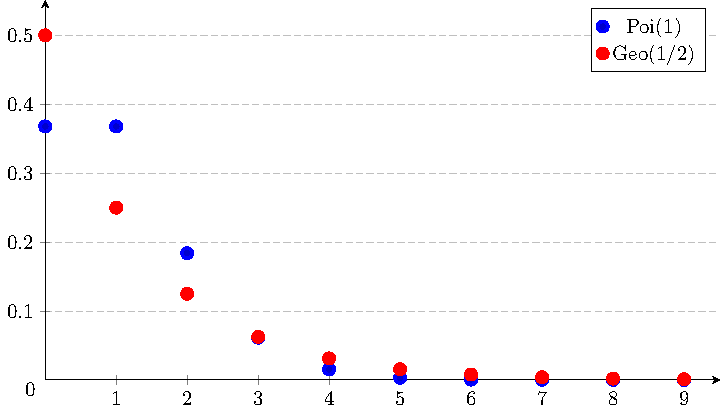
\includegraphics[width=\columnwidth]{./figures/appendix/poi_geo_plot.pdf}
    \caption{Our geometric distribution $p$ and Poisson fit $q$.}
    \label{fig:poi_geo_plot}
\end{figure}

For $\lambda=1$ we compute a cross-entropy of
$$
H(p,q;1)
=
1+\sum_{k=1}^{\infty}\frac{\log(k!)}{2^k}
\approx
2.01567.
$$
On its own, this quantity isn't too useful. To get a sense of goodness-of-fit we desire the KL-divergence, i.e. the cross-entropy minus the self-entropy of $p$. Let's compute said self-entropy:
\begin{align*}
    H(p)
    &=
    -\sum_{k=1}^{\infty}p(k)\log(p(k))\\
    &=
    -\sum_{k=1}^{\infty}2^{-k}\log(2^{-k})\\
    &\approx
    1.386
\end{align*}
from which we know that the KL-divergence between the underlying geometric distribution $p$ and our Poisson fit $q$ is given by
$$
\text{KL}(p||q)
\approx
2.016-1.386
=
0.63.
$$

\subsection{Pearson Correlation and Mutual Information}
\label{app:pearson_correlation}
If $X$ and $Y$ are scalar random variables then their Pearson correlation is given by
$$
\rho_{X,Y}
=
\frac{\E\l[(X-\E[X])(Y-\E[Y])\r]}{\sqrt{\E\l[(X-\E[X])^2\r]\E\l[(Y-\E[Y])^2\r]}}
=
\frac{\text{Cov}(X,Y)}{\sigma_X\sigma_Y}
\in[-1,1]
$$
where the expectation in the numerator is over their joint $p_{(X,Y)}$. The overall quantity yields the linear dependence between $X$ and $Y$ and the denominator is for normalisation.

What if we want an idea of the non-linear dependence between random variables? This desire motivates mutual information. The mutual information of the joint over $\X$ and $\mathbf{Y}$ is often spoken of as a property of two random variables $\X$ and $\mathbf{Y}$ and is denoted as such as in
$$
I(\X;\mathbf{Y})
=
D_{\text{KL}}(p_{\X,\mathbf{Y}}||p_{\X}\otimes p_{\mathbf{Y}}).
$$
I'm massively in favour of writing it as a KL-divergence as its meaning is immediately clear: its a measure of divergence between the joint and the product of the marginals. Informally, I see it as asking ``How well does the product of marginals model the joint?'' which is precisely the question we seek to answer when utilising things like Pearson correlation and mutual information.

\subsection{Quality of fit $\approx$ Encoding quality?}
\TODO Perhaps worthy of its own section, unsure

% classical statistics things
\section{Classical Statistics Things}
Here are some classical statistics things.

\subsection{Sample Independence}
The intended meaning of the term `sample' in statistics is a set of independently obtained realisations of a random variable, i.e. $\{\x_1,\dots,\x_n\}\overset{i.i.d.}{\subset}\Omega_{\X}$. You could also define a sample as a set of i.i.d. random variables $\{\X_1,\dots,\X_n\}$. There are times where it's more useful to refer to sets of i.i.d. random variables but I more often reason with their realisations when using sample as a term. It can be especially confusing when context switching between machine learning and classical statistics. In the context of machine learning, a sample is intended to mean a single data point, while in classical statistics it is what's written above. This was a huge cause of confusion during a few meetings with my master's thesis supervisor who is a Bayesian statistician.

As for sample independence, I always default to thinking of the following simple example. Suppose we'd like to estimate the population mean of the heights of men and women. If we randomly sample 100 men and 100 women separately then the sample mean serves as a fine estimate. This could computed by independently sampling, without replacement, from the categorical distribution corresponding to ID numbers of all individuals in the population. If we instead randomly sampled 100 couples then the obtained samples would not be independent as heights of couples correlate. Sample independence is a key assumption made in many estimation methods, e.g. maximum likelihood estimation.

\subsection{Estimators}
Suppose you have a bunch of i.i.d. random variables $\X_1,\dots,\X_n$, an estimator is a function $\hat{\theta}:\Omega_{\X}^n\to\mathbb{R}^k$. Given the sample $\{\x_1,\dots,\x_n\}\subset\Omega_{\X}$, the value $\hat{\theta}(\x_1,\dots,\x_n)$ is typically denoted by $\hat{\theta}$ for shorthand and is referred to as an estimate. The reason that this lack of rigour in notation is allowable is that the contexts in which it is used often make it clear when an estimator is being considered as opposed to an estimate, and vice versa.

The simplest example of a often-used estimator is the estimator of the mean as in
$$
\hat{\mu}(\X_1,\dots,\X_n)
=
\frac{1}{n}\sum_{i=1}^n \X_i.
$$
In this case, the dimension of the codomain of $\hat{\mu}$ is simply the dimension of the sample space of $\X$. Given a sample $\{\x_1,\dots,\x_n\}$, an estimate of the mean of the corresponding distribution is given by $\hat{\mu}=\frac{1}{n}\sum_{i=1}^n\x_i$.

\subsubsection{(Estimator) Bias}
Given that estimators are simply statistics used to approximate some quantity of the corresponding distribution, a natural question is how to measure the goodness of an estimator. The most well known such measure is the bias of an estimator in estimating a quantity $\theta$ given by
$$
\text{Bias}(\hat{\theta})
=
\E[\hat{\theta}]-\theta
$$
where the expectation is with respect to $p_{\X}^{{\otimes}n}$. The need for the precise terminology `in estimating a quantity $\theta$' is because one could, for example, use the sample mean as an estimator of both the population mean and the population variance (as ridiculous as this choice may be for the latter). As an estimator of the population mean, the sample mean is unbiased. Not so much for the latter. That said, an estimator being unbiased does not necessitate that it is `good'. For example, if you had $X_1,\dots,X_n\overset{\text{i.i.d.}}{\sim}\text{Ber}(p)$ then $X_1$ is an unbiased estimator of $p$. To follow this, there are strange special cases in which every unbiased estimator of a quantity is worse than many biased estimators.

As an example of computing the bias of an estimator, see that the sample mean is an unbiased estimator of the population mean $\mu$ as
\begin{align*}
    \text{Bias}(\hat{\mu})
    &=
    \E[\hat{\mu}]-\mu\\
    &=
    \E\l[\frac{1}{n}\sum_{i=1}^n\X_i\r]-\mu\\
    &=
    \frac{1}{n}\sum_{i=1}^n\E[\X_i]-\mu\\
    &=
    0.
\end{align*}
It turns out that the most natural estimator of population variance $\sigma^2$, given by
$$
\frac{1}{n}\sum_{i=1}^n\l(\X_i-\hat{\mu}\r)^2,
$$
is biased. This can be seen after a bunch of tedious computations which yield a bias of $-\sigma^2/n$. To account for this, an unbiased estimator of the population variance is given by
$$
\hat{\sigma}^2
=
\frac{1}{n-1}\sum_{i=1}^n\l(\X_i-\hat{\mu}\r)^2.
$$
Most of the time, `sample variance' refers to the unbiased estimator.

\subsubsection{Sampling bias}
For a given estimator, sampling bias is not its bias as an estimator but instead the bias induced due to samples being drawn from a distribution $q_{\X}^{\otimes n}$ which is distinct from the true distribution $p_{\X}^{\otimes n}$ as in $\E_{q_{\X}^{\otimes n}}[\hat{\theta}]-\theta$. Note that this is not an issue of a given estimator and is instead an issue with the `data collection' procedure. 

\subsubsection{Efficiency}

\subsubsection{Consistency}

\subsubsection{Sufficiency}

\subsection{Hypothesis Testing}

\subsection{Markov Chain Monte Carlo (MCMC) Methods}
There are a fair number of scenarios in which it's desirable to sample from a distribution whose probability function can only be evaluated up to a constant. As an example, the posterior
$$
p(\theta|D)
=
\frac{p(D|\theta)p(\theta)}{p(D)}.
$$
whose explicit evaluation is difficult due to the constant $p(D)$. MCMC methods help remedy this issue.

\subsubsection{Markov Chains}
It's helpful to first understand Markov chains. A markov chain is a discrete-time stochastic process in which the sample space is countable and the Markov property
$$
p(x_{n+1}|x_1,\dots,x_n)
=
p(x_{n+1}|x_n)
$$
holds for all $n\in\mathbb{N}$. To make notation more convenient, let
$$
p_{i,j}
:=
p(x_{n+1}=j|x_n=i).
$$
The great thing about Markov chains is how elegantly we can write $p(x_{n+1}=j)$ in terms of the distribution over $\X_n$ as in
\begin{align*}
    p(x_{n+1}=j)
    &=
    \sum_{i=1}^{|\Omega_X|} p(x_n=i,x_{n+1}=j)\\
    &=
    \sum_{i=1}^{|\Omega_X|} p(x_{n+1}=j|x_n=i)p(x_n=i)\\
    &=
    \sum_{i=1}^{|\Omega_X|} p_{i,j}\cdot p(x_n=i).
\end{align*}
If $\pi^{(n)}=\begin{bmatrix} p(x_n=1) & p(x_n=2) & \dots & p(x_n=|\Omega_X|)\end{bmatrix}$ and
$$
P
=
\begin{bmatrix}
    p_{1,1}          & \dots  & p_{1,|\Omega_X|}\\
    \vdots           & \ddots & \vdots          \\
    p_{|\Omega_X|,1} & \dots  & p_{|\Omega_X|, |\Omega_X|}
\end{bmatrix}
$$
then the transition equation above reduces to
$$
\pi^{(n+1)}
=
\pi^{(n)}P
$$
If each $p_{i,j}$ is known beforehand and an initial distribution $X_0\sim\pi^{(0)}$ is attributed then the distribution at step $n$ is given by
$$
\pi^{(n)}
=
\pi^{(0)}P^n.
$$
A distribution $\pi$ is said to be stationary with respect to the transition matrix $P$ if
$$
\pi
=
\pi P.
$$

\begin{example}
    Suppose tomorrow's weather is entirely determined by today's weather and that the weather can only be sunny or rainy. Further, suppose that the transition probabilities are given by
    $$
    p(S|S)=0.8\quad
    p(S|R)=0.4\quad
    p(R|S)=0.2\quad
    p(R|R)=0.6
    $$
    and that today is sunny, so $x_0=S$. The distribution over weather types two days from now is thus
    $$
    \pi^{(2)}
    =
    \pi^{(0)}P^2
    =
    \begin{bmatrix}1&0\end{bmatrix}
    \begin{bmatrix}
        0.8 & 0.2\\
        0.4 & 0.6
    \end{bmatrix}^2
    =
    \begin{bmatrix}0.72&0.28\end{bmatrix}.
    $$
    To find the stationary distribution with respect to $P$ simply compute a left eigenvector.
\end{example}

\subsubsection{Metropolis-Hastings}

\begin{figure}[t]
    \centering
    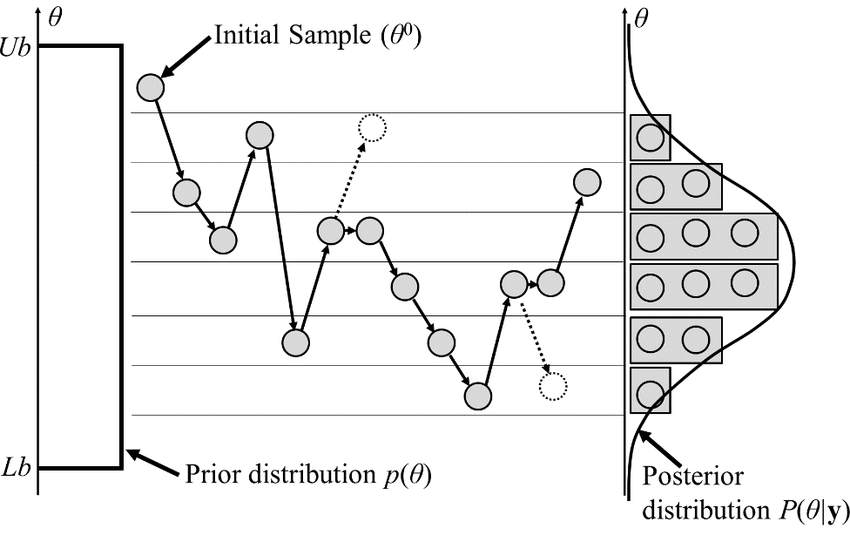
\includegraphics[width=\columnwidth]{./figures/appendix/metropolis-hastings.png}
    \caption{Metropolis-Hastings in action with a uniform prior.}
    \label{fig:metropolis_hastings}
\end{figure}

\subsubsection{Gibbs sampling}
When the joint $p(x_1,\dots,x_m)$ is hard to sample according to but the conditionals
$$
p(x_i|x_1,\dots,x_{i-1},x_{i+1},\dots,x_m)
=:
p(x_i|x_{-i})
$$
are not hard to sample according to, a nice approach to sampling from the joint is Gibbs sampling. The idea is to iteratively sample from the conditionals to obtain a full samples by initialising $\l(x_1^{(0)},\dots,x_m^{(m)}\r)$ and sampling
$$
x_1^{(1)}\sim p\l(x_1^{(0)}|x_{-1}^{(0)}\r).
$$
The idea is intuitive and theory surrounding it offers certain guarantees as far as sampling quality goes. I'm only interested in the intuition of it.

As an example, consider
$$
(X_1,X_2)
\sim
\mathcal{N}\l(\begin{bmatrix} 0 \\ 0 \end{bmatrix}, \begin{bmatrix}1 & 1/2\\ 1/2 & 1\end{bmatrix}\r).
$$
The conditional distributions relevant to Gibbs sampling are
$$
X_1|(X_2=x_2)\sim\mathcal{N}\l(\frac{x_2}{2},\frac{3}{4}\r)
\hfill
\quad\text{and }\quad
X_2|(X_1=x_1)\sim\mathcal{N}\l(\frac{x_1}{2},\frac{3}{4}\r).
$$
So instead of sampling according to the joint $p(x_1,x_2)$, repeatedly sample according to conditionals $p(x_1|x_2)$ and $p(x_2|x_1)$.

\subsection{Hidden Markov Models (HMMs)}

\subsection{The Curse of Dimensionality}
Unsure where to place this tbh

\subsubsection{The blessing of non-uniformity}

\subsection{The Expectation-Maximisation (EM) Algorithm}
Maximum likelihood estimation (MLE) is great but what do we do when the data generating process is not determined entirely by observed model variables $\X=(X_1,\dots,X_m)$. That is, what if $p(\x)$ is simply the marginal of the true joint $p(\x,\z)$ where $\Z=(Z_1,\dots,Z_{m'})$ are hidden variables?

It turns out that there's a clever way of perfmorming MLE while accounting for hidden variables called the expectation-maximisation (EM) algorithm. It involves obtaining a lower bound for the log-likelihood of a given sample of the observed variables and instead maximising the lower bound in the model's parameters. If certain conditions are met for said lower bound to in fact reach equality with the sample's log-likelihood then the application of EM is MLE itself. If the bound is not exact then we refer to the process as variational EM.

In obtaining a lower bound, let $\theta$ denote the parameters of the true joint $p_{\theta}(\x,\z)$ and see that if $q$ is a probability mass function with domain $\Omega_{\Z}$ then
\begin{align*}
    \log(p_{\theta}(\x))
    &=
    \log\l(\sum_{\z\in\Omega_{\Z}}p_{\theta}(\x,\z)\r)\\
    &=
    \log\l(\sum_{\z\in\Omega_{\Z}}q(\z)\frac{p_{\theta}(\x,\z)}{q(\z)}\r)\\
    &=
    \log\l(\E_{\Z\sim q}\l[\frac{p_{\theta}(\x,\Z)}{q(\Z)}\r]\r)\\
    &\geq
    \E_{\Z\sim q}\l[\log\l(\frac{p_{\theta}(\x,\Z)}{q(\Z)}\r)\r]\\
    &=
    \E_{\Z\sim q}\l[\log\l(p_{\theta}(\x,\Z)\r)\r]+H(q)\\
    &=:
    \text{ELBO}(q,\theta)
\end{align*}
in which `ELBO' stands for evidence lower bound (swap the sums for integrals if you'd like continuously distributed hidden variables). Note that this is not the same ELBO dervied in motivating variational autoencoders (VAEs).

The EM algorithm performs coordinate ascent (component-wise equivalent of gradient ascent) on the ELBO: iteratively maximising $\text{ELBO}(q,\theta)$ in $q$ (with $\theta$ fixed) and then in $\theta$ (with $q$ fixed) until some convergence crtieria is met. With $q$ fixed, maximising the ELBO in $\theta$ amounts to computing
\begin{align*}
    \argmax_{\theta}\text{ELBO}(q,\theta)
    &=
    \argmax_{\theta}\E_{\Z\sim q}\l[\log\l(p_{\theta}(\x,\Z)\r)\r]\\
    &=
    \argmax_{\theta}\Big(\E_{\Z\sim q}\l[\log\l(p_{\theta}(\x|\Z)\r)\r]+\E_{\Z\sim q}\l[\log\l(p_{\theta}(\Z)\r)\r]\Big)\\
    &=
    \argmax_{\theta}Q(\theta;q)
\end{align*}
where $Q(\theta;q)=\E_{\Z\sim q}\l[\log\l(p_{\theta}(\x|\Z)\r)\r]+\E_{\Z\sim q}\l[\log\l(p_{\theta}(\Z)\r)\r]$. Note that equality is offered by the bound precisely when $q(\z)=p_{\theta}(\z|\x)$ and so, with $\theta$ fixed, maximising the ELBO in $q$ amounts to computing
$$
\argmax_{q}\text{ELBO}(q,\theta)
=
p_{\theta}(\z|\x),
$$
i.e. computing the posterior.

With both statements in mind, the EM algorithm amounts to initialising the parameters $\theta^{(0)}$ and repeating the following two steps from $t=0$ until stopping criteria is met:
\begin{enumerate}
    \item (E step: $\theta^{(t)}\to q_t$) Obtain a closed form for $q_t(\z)=p_{\theta^{(t)}}(\z|\x)$ and in turn a closed form for $Q(\theta;q_t)$
    \item (M step: $q_t\to\theta^{(t+1)}$) Compute $\theta^{(t+1)}=\argmax_{\theta}Q(\theta;q_t)$
\end{enumerate}

\begin{tcolorbox}[title={\centering\textbf{Variational EM}}, colback=myLightBlue, colbacktitle=myDarkBlue, colframe=myDarkBlue, coltitle=white]
    Computing the posterior exactly is often infeasible in practice. Varational EM seeks to alleviate this by instead restricting $q$ to a family of functions $\mathcal{F}$, e.g. some family of MLPs, and replacing the E-step with the computation
    $$
    q_t
    =
    \argmax_{q\in\mathcal{F}}\text{ELBO}\l(q,\theta^{(t)}\r).
    $$
    Of course, if the posterior $p_{\theta^{(t)}}(\z|\x)$ belongs to $\mathcal{F}$ for all relevant $t\in\mathbb{N}$ then variational EM is simply EM.
\end{tcolorbox}
Regarding the correctness of the EM algorithm, we seek to show that
$$
\log(p_{\theta^{(t+1)}}(\x))
\geq
\log(p_{\theta^{(t)}}(\x))
$$
for all $t\in\mathbb{N}$, i.e. individual steps in the loss landscape are neglible at worst and otherwise increase the likelihood of the observed data. Showing this turns out to be elegant, as in
$$
\log(p_{\theta^{(t+1)}}(\x))
\geq
\text{ELBO}\l(q_t,\theta^{(t+1)}\r)
\geq
\text{ELBO}\l(q_t,\theta^{(t)}\r)
=
\log(p_{\theta^{(t)}}(\x)).
$$
The leftmost inequality is due to how the ELBO is defined. The second inequality is seen from
$$
\theta^{(t+1)}
=
\argmax_{\theta}\text{ELBO}\l(q_t,\theta\r).
$$
Finally, the equality follows from the `matching the true posterior with $q_t$' argument offered earlier, i.e.
$$
q_t(\z)=p_{\theta^{(t)}}(\z|\x)
\implies
\text{ELBO}\l(q_t,\theta^{(t)}\r)=\log(p_{\theta^{(t)}}(\x)).
$$

% bayesian things
\section{Bayesian Persuasion}
Bayes' law states that for events $A$ and $B$ with $p(B)\neq0$
$$
p(A|B)
=
\frac{p(B|A)p(A)}{p(B)}.
$$
I sometimes refer to it as Bayes' theorem (as do others) but since it follows straightforwardly from the definition of conditional probabilities, I prefer to refer to it as a law/identity. It's particularly useful when $p(B|A)$ is a natural quantity and accessible while $p(A|B)$ is not a natural quantity but is desired.

Another worthwhile point is that it's fairly common that someone with malicious intent emphasies how high or low $p(A|B)$ is when in fact $p(B|A)$ is the quantity that should motivate the argument at hand. Unforuntately, human intuition for which conditional probability is relevant to their argument is very bad.
\begin{example}
    Being infected with HIV and testing positive for HIV.
\end{example}

\subsection{Posetriors Over Parameters}
Treat parameters as random variables as opposed to a point estimate. Get a distribution over them given data, as in
$$
p(\theta|D)
=
\frac{p(D|\theta)p(\theta)}{p(D)}.
$$
Posetrior, likelihood, prior and marginal likelihood.

\begin{example}
    Beta-binomial
\end{example}

\subsection{Variational Bayesian inference}
Instead of approximating the posterior via MCMC, one can restrict the approximation to a function family and minimise some divergence measure, e.g. KL-divergence. The name `variational' derives from calclulus of variations as in computing
$$
q^*
=
\argmax_{q\in\mathcal{Q}}\mathcal{L}(q)
$$
where $\mathcal{L}$ is a functional.

% % philosophy things
% \section{Philosophy Things}
% I don't think about the philosophic aspects of maching learning very often as I'm in the camp of people whose interests lie in solving present problems. I find some topics interesting though.

% % thoughts on reasoning
% \subsection{Thoughts on reasoning (Summer 2024)}

% At the time of writing, machine learning, as a term, is used almost interchangeably with artificial intelligence (AI). AI isn't particularly well-defined in itself, even in academic settings, so its use in day-to-day things, e.g. in the news, often causes confusion and debate. I'm not sure how I would define AI in a way that'd satisfy most. Maybe the discipline of studying things that can `reason', as a human does, given some agreed upon notion of `reasoning'. A common issue found in discussions surrounding this topic is that a definition of `reasoning' is left out.

% Right now, I'm unaware of any machine learning model that can `reason' by any agreed upon definition of the term. I suspect that while current models can simulate `reasoning' to the extent of being able to effectively solve tasks which require some sort of underlying understanding, they do not `reason' in the human sense, which is grounded in embodied experience. Let's say that an LLM (e.g. GPT-4o) concludes that a continuous real-valued function $f:\R\rightarrow\R$ has a root in some interval $(a, b)$ using the intermediate value theorem (IVT) by noting that $f(a)<0$ and $f(b)>0$. Did the LLM `reason' in its application of the IVT or do we instead brush this off as the LLM having been trained on many examples of the application of the IVT? Does it `understand' what it's concluding? As of right now I'd say that it doesn't. This of course isn't something unique to the IVT — we can construct many such examples. What I think makes the IVT interesting is that we can effectively express what it means to `understand' its correctness as a human. I'd say that the distinction between the LLM's `understanding' and a human's here is that a human knows that if they trace their finger on a piece of paper starting from the bottom half, crossing a horizontal line cutting through the middle of the paper, to the top half of the paper without removing their finger then their finger must have touched the horizontal line at some point (ignore the fact that such a traversal is not necessarily a function, you get the idea). You don't need any mathematical training to know and, more importantly, understand why your finger crosses through the horizontal line on the page. LLMs certainly do not `understand' the correctness of the IVT in this way, or really any way that isn't purely symbolic. Maybe multimodal LLMs will alleviate this.

% A separate but related question is to what extent it matters that a model `reasons' in order to arrive its conclusions. Somewhat in the same way that it doesn't matter that a calculator has no inherent idea of why it outputs 6 when you input $3\cdot2$. From a purely problem solving point of view, these philosophical debates regarding what constitutes reasoning, understanding and knowing aren't too important in the short term. It'd be funny if 50 years from now we're well-taken care of by a fleet of machine learning-powered robots and we still look down on them for not being capable of true reasoning.

% \subsection{Sufficiency of Internet-Scraped Data}
% \TODO 

% \subsection{The Principled Measure-Explainability Tradeoff}
% \TODO 

\end{appendices}

\end{document}
